% Sample Dissertation, Thesis, or Document %
%            for use with the              %
%  University of Arizona Thesis Class,     %
%               uathesis.cls               %
%------------------------------------------%

% We'll use the uathesis document class (duh).  The uncommented line
% below will produce a Dissertation, the others would produce a Thesis
% or a Document.  There are other options available to you like turning
% on the copyright statement and replacing the year on the title page
% with a "generated on" stamp (handy for early drafts).  To find out
% what the available options are, take a look into the uathesis.cls
% file and look for the \DeclareOption commands near the top of that
% file.
% There are five copyright options.  Copyright, no copyright, and three
% different Creative Commons licences.  Use the one you want (If you go
% Creative Commons, I (DM) think the CC-BY-ND makes the most sense)  See
% uathesis.cls for the reason why the non-commercial licenses are not
% included.
\documentclass[dissertation]{uathesis}
%\documentclass[dissertation,copyright]{uathesis}
%\documentclass[dissertation,CC-BY]{uathesis}
%\documentclass[dissertation,CC-BY-SA]{uathesis}
%\documentclass[dissertation,CC-BY-ND]{uathesis}
%\documentclass[thesis]{uathesis}
%\documentclass[document]{uathesis}

% Package Usage
% These are the packages that we need
\usepackage{graphicx}
\usepackage[square,numbers]{natbib}
\usepackage[titles]{tocloft}
\usepackage{amsmath}
\usepackage{amssymb}
\usepackage{epstopdf}
\usepackage{dcolumn}% Align table columns on decimal point
\usepackage{bm}% bold math
\usepackage{setspace}
\usepackage{rotating}
\renewcommand*\cftfigpresnum{Figure~}
\setlength{\cftfignumwidth}{5.5em}
\renewcommand\cftchapfont{\normalfont}
\renewcommand\cftchappagefont{\normalfont}
\renewcommand\cftchapleader{\cftdotfill{\cftsecdotsep}}

\newcommand\alphaNa{\alpha_\textrm{Na}}
\newcommand\alphaK{\alpha_\textrm{K}}
\newcommand\alphaRb{\alpha_\textrm{Rb}}
\newcommand\alphaCs{\alpha_\textrm{Cs}}
\newcommand\lambdaZero{\lambda_\textrm{zero}}

\newcommand*{\etal}{\emph{et al.}~}

\newcommand{\tensorPol}{\overset{\leftrightarrow}{\alpha}}

			% natbib is available on most systems, and is
					% terribly handy.
					% If you want to use a different Bibliography package, 
					% you should be able to, just change this
					% and the \bibliographystyle command below.  Be warned
					% that you may need to do a little hacking to get
					% the REFERENCES item to show up in your TOC.

% Compatibility with the AASTEX package 
% of the American Astronomical Society.
%\usepackage{deluxetable}		% Allows use of AASTEX deluxe tables
%\usepackage{aastex_hack}		% Allows other AASTEX functionality.

% These are other packages that you might find useful.
% For controlling the fonts, see
% http://www.math.uiuc.edu/~hartke/computer/latex/survey/survey.html
% The following is a nice font set:
%\usepackage{mathtime}			% Times for letters; Belleek math.
%
\usepackage{amsmath}			% AMS Math (advanced math typesetting)
%\usepackage{lscape}			% Used for making fitting large tables in by putting them landscape
%\usepackage{refs}			
%
% If you are using hyper-ref (recommended), this command must go after all 
% other package inclusions (from the hyperref package documentation).
% The purpose of hyperref is to make the PDF created extensively
% cross-referenced.
\usepackage[pdftex,bookmarks,colorlinks=true,urlcolor=black,linkcolor=black,citecolor=black]{hyperref}

% Set up some values
\completetitle{Polarizability and magic-zero wavelength measurements of alkali atoms}
\fullname{William Frederick Holmgren}			% Grad college wants your full name here.
\degreename{Doctor of Philosophy}	% Title of your degree.

\begin{document}
\newcommand{\beq}{\begin{eqnarray}}
\newcommand{\eeq}{\end{eqnarray}}
\newcommand{\ii}{{\mathrm i}}

% Set up the title page
\maketitlepage
{DEPARTMENT OF PHYSICS}	% Title of your department.
{2013}							

% Insert the approval form.  Note that for electronic submission
% of your Ph. D. dissertation, you must bring *two* copies of the
% approval page to your final defense.  These must be signed by
% the committee.  Make two photocopies: one for Pam and the other
% for your records.  Then, bring the two signed originals to the
% graduate college when you submit the final version of the
% dissertation to the University of Arizona.
\approval
{2 April 2013}		% Defense Date	
{Alexander D. Cronin}	% Dissertation Director
{Alexander D. Cronin}	% 1st committee member
{Arvinder Sandhu}		% 2nd committee member
{Charles S. Stafford}		% 3rd committee member
{Brian P. Anderson}		% 4th committee member

% Include the ``Statement by Author'' for Dissertations
\statementbyauthor
% If this is a Thesis, use the following form, with your thesis director's
% name and title in the square brackets like so (you should also omit the 
% approval form insertion above):
%\statementbyauthor[Jane M. Doe\\Professor of Chemistry]

% Include the ``Acknowledgements''
%\incacknowledgements{acknowledgements}

% Include the ``Dedication''
%\incdedication{dedication}

% Create a ``Table of Contents''
\tableofcontents

% Create a ``List of Figures''
\listoffigures

% Create a ``List of Tables''
\listoftables

% Include the ``Abstract''
\incabstract{abstract}

% Include the various chapters
\chapter{INTRODUCTION}


What happens to an atom in an electric field? An atom is a neutral particle so it will not accelerate in a uniform electric field, however, it is composed of positively charged protons and negatively charged electrons that do feel electric forces. If we place our test atom in a charged parallel-plate capacitor, the negatively charged electrons tend to move toward the positively charged surface, while the much heavier and positively charged nucleus moves only slightly toward the negatively charged surface. As a result of these movements, the atom becomes stretched out by an amount determined by its \emph{polarizability}. Figure \ref{simplePolFig} shows a cartoon of this idea. The polarizability of a spherical particle is proportional to its volume and this remains approximately true for atoms as well. As such, polarizability is conveniently expressed in terms of a volume, typically $a_0^3$ or 10$^{-24}$ cm$^3$. The SI unit of polarizability, C m$^2$/V, can be reduced to a volume by simply dividing by $4\pi\epsilon_0$. 


\begin{figure}
\centerline{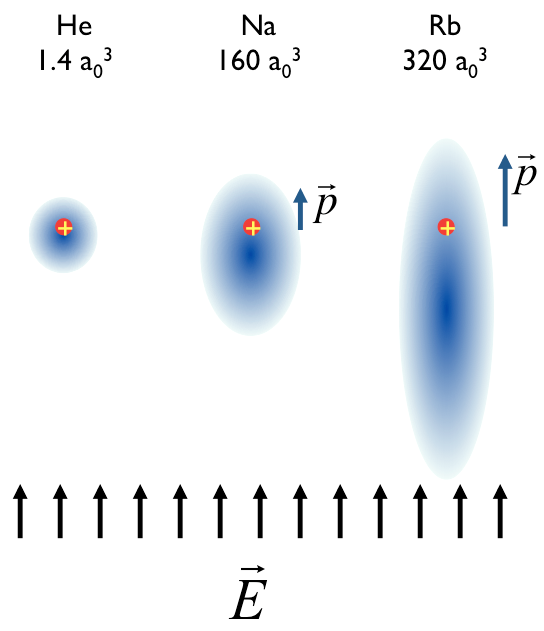
\includegraphics[width=0.5\textwidth]{Figures/simplePolFigv2.png}}
\caption[An electric field applied to an atom induces a dipole moment in proportion to its atomic polarizability.]{\label{simplePolFig}An electric field applied to three different atoms, helium, sodium, and rubidium, induces a dipole moment in proportion to the atomic polarizability. The polarizability roughly scales in proportion to the volume of the atom.}
\end{figure}


More precisely, the polarizability $\alpha$ of an atom relates the induced dipole moment $\vec{p}$ to the applied electric field $\vec{E}$ by
\begin{eqnarray}
\vec{p} = \alpha \vec{E} +  ...
\end{eqnarray}
The dipole moment is $\vec{p}=e\vec{r}$, where $\vec{r}$ is the displacement of the electron cloud. Higher order terms, such as the hyperpolarizability, will be neglected in this work since we operate our experiments at more than $10^5$ times below the scale of the atomic field ($\vec{E}_a \approx e/a_0^2=5\times10^{11}$ V/m). 


The energy shift of a polarizable particle in an electric field is given by
\begin{eqnarray}
\label{starkShift}
U = -\frac{1}{2} \alpha \vec{E}^2,
\end{eqnarray}
and this is commonly referred to as the Stark shift. Polarizability can also be defined through 2nd-order perturbation theory. The Hamiltonian of a polarizable particle is
\begin{eqnarray}
H = H_\textrm{atom} - \hat{p} \cdot \vec{E}
\end{eqnarray}
where $\hat{p}$ is the dipole operator. Application of 2nd order perturbation theory leads to a ground-state static polarizability of
\begin{eqnarray}
\label{pertubationTheoryEqn}
\alpha = 2e^2 \sum_{i\neq0} \frac{ | \langle i | \vec{r} . \vec{E} | 0 \rangle |^2}{E_i}
\end{eqnarray}
where $e$ is the electron charge and $E_i$ is the energy of the $i$th atomic state, assuming $E_0 \equiv 0$. So far we have assumed that the applied field is constant in time, but we will examine the frequency dependence of the dynamic polarizability in sections \ref{mzwBrief} and \ref{dynPolSec}.


Equation \ref{pertubationTheoryEqn} gives us insight into why polarizability is an interesting property to study: it can be expressed as a sum of dipole matrix elements. These matrix elements also describe properties such as transition strengths, state lifetimes, van der Waals interactions, indices of refraction, and scattering cross-sections, just to name a few. In fact, in a 1966 review of atomic polarizabilities, Bederson and Robinson referred to polarizability as a ``seemingly ubiquitous parameter" \cite{Bed66} and T.M.~Miller compiled a list of properties directly related to polarizability with more than 15 entries \cite{Mil12}. Since dipole matrix elements are notoriously difficult to calculate, experiments such as the ones described in this thesis can serve as input to a long list of calculations.


New applications of atomic physics continue to demand better knowledge of atomic polarizabilities. Next generation optical lattice clocks based on strontium and ytterbium atoms suffer from significant frequency shifts due to blackbody radiation and accurate calibration of these frequency shifts requires precise knowledge of polarizabilities \cite{Lud08,Der11}. Parity non-conservation studies \cite{Woo97,Tsi09} using atomic systems impose limits on physics beyond the standard model, but require accurate atomic structure calculations to interpret the measurements \cite{Der07}. Polarizability measurements are some of the best ways to test these calculations.


This thesis describes three experiments all concerned with precisely answering the seemingly simple question of what happens to an atom in an electric field. The most important findings are as follows:
\begin{itemize}
\item I used an atom interferometer and a novel electric field gradient geometry to measure the polarizabilities of K and Rb with unprecedented precision (0.5\% uncertainty) \cite{Hol10}. These measurements are now listed in the CRC Handbook of Chemistry and Physics, and they establish a roadmap for future polarizability measurements in our lab.
\item I developed a new technique to measure atom beam velocities with 0.1\% uncertainty using phase choppers \cite{Hol11}. This technique will enable more precise polarizability measurements.
\item I measured a wavelength, referred to as a magic-zero wavelength, for which the dynamic polarizability of potassium equals zero. We measured the first, i.e.~the longest, magic-zero wavelength of potassium with 1.5 pm uncertainty \cite{Hol12a}. I explain how this is a novel method to test atomic structure calculations and also establishes a foundation for future measurements of magic-zero wavelengths in our lab.
\end{itemize}



The remainder of this introduction provides a brief history of polarizability measurements and a review of the basic matterwave optics needed for understanding the experiments in this thesis. Chapter 2 summarizes the experiments, papers, and proposals that comprise this thesis work. Chapters 3-5 provide supporting material for our peer-reviewed publications on static polarizability measurements of Na, K, and Rb (Appendix A) \cite{Hol10}, a new atom velocity measurement technique using phase choppers that will improve polarizability measurements (Appendix B) \cite{Hol11}, and a measurement of the first magic-zero wavelength of the dynamic polarizability of potassium (Appendix C) \cite{Hol12a}. Chapters 6 and 7 propose two new experiments: measurements of Sr polarizability using a resonant photoionization detector and measurements of the tensor polarizabilities of alkali dimers.








%%%%%%%%%%%%%%%%%%%%%%%%%%%%%%%%%%%%%
\section{A brief history of polarizability measurements}
\label{introPolHistory}
In this section we provide a brief review of the history of polarizability measurements. For comprehensive reviews of polarizability measurements, see Mitroy, Safronova and Clark (2010) \cite{Mit10}, Gould and Miller (2005) \cite{Gou05}, Hohm (2000) \cite{Hoh00}, Miller and Bederson (1989) \cite{Mil89}, Miller and Bederson (1978) \cite{Mil78}, Bederson and Robinson (1966) \cite{Bed66}, and the CRC Handbook of Chemistry and Physics \cite{Mil12}. 

Scheffers and Stark started the business of polarizability measurements in 1934 \cite{Sch34} by deflecting atomic beams of Li, K, and Cs in an inhomogenous electric field. More than 25 years later, Benjamin Bederson developed the E-H gradient spectrometer at NYU \cite{Bed60} and in 1961 made the first measurements of polarizabilities since Stark \cite{Sal61}. These measurements were made with about 15\% uncertainty and formed the foundation for a career's worth of impressive polarizability measurements discussed below. 

In 1974, \emph{Physical Review A} published two landmark polarizability measurement papers. Hall and Zorn \cite{Hal74} measured the polarizabilities of the alkalis Na through Cs with 7\% uncertainty using beam deflection, and Molof, Schwartz, Miller, and Bederson \cite{Mol74} measured the polarizabilities of Li through Cs and the $^3\textrm{P}_2$ metastable nobel gas atoms with 2\% uncertainty using the E-H gradient balance technique. Molof \etal provided measurements of polarizability unmatched for over 2 decades and has been cited over 200 times. Molof \etal achieved their relatively low uncertainties by measuring polarizabilities with respect to the polarizability of metastable He, which can be calculated with high precision. In this thesis, we continue the technique of using ratio measurements of polarizabilities for improved precision.

The Bederson group also measured the average dipole polarizabilities of homonuclear alkali dimers with 10\% uncertainty in 1974 by using ratios with respect to the polarizabilities of the alkali atoms \cite{Mol74a}. The polarizabilities of Ba, Sr \cite{Sch74} and Ca \cite{Mil76} were also measured with respect to Li over the next two years. In 1993, Tarnovsky \etal measured the polarizabilities of both the homonuclear and heteronuclear alkali dimers with Bederson \cite{Tar93}. These measurements were made with 6-10\% uncertainty.

The 1990s saw the advent of atom interferometry and its promise of high precision measurements of atomic properties \cite{Eks95, Mif06, Lep11a}, fundamental constants of nature \cite{Fix07}, and inertial displacements \cite{Len97, Gus97}. The Pritchard group at MIT made the first interferometry-based precision polarizability measurement of an atom, Na, with 0.35\% uncertainty using a three nanograting Mach-Zehnder atom interferometer \cite{Eks95}. In Toulouse, the Vigu\'{e} group measured the polarizability of Li with 0.66\% uncertainty using an atom beam interferometer with light gratings \cite{Mif06}. The Arndt group in Vienna measured the polarizability of $C_{60}$ and $C_{70}$ with 6\% uncertainty and their ratio with 2.5\% uncertainty using a near field interferometer \cite{Ber07}. 

The development of laser trapping and cooling enabled several new polarizability measurements, as well. The Sackett group in Virginia measured the dynamic polarizability of Rb near the D1 and D2 lines with 7\% uncertainty using a guided ultracold atom interferometer \cite{Dei08}. Amini and Gould used an atomic fountain to measure the polarizability of Cs with 0.14\% uncertainty \cite{Ami03}. This measurement provides a valuable benchmark for calculations \cite{Der07, Por09} needed to interpret atomic parity non-conservation experiments \cite{Woo97}. Cold atom experiments offer much longer interaction times than atom beam experiments and ultracold atom interferometers may offer better than shot-noise limited precision. However, these experiments often suffer from additional systematic errors, such as density-dependent phase shifts, and therefore independent measurements provide valuable cross-checks. 

Other notable measurements of polarizabilities of non-alkali or alkaline-earth atoms include the following. Sch\"{a}fer \etal measured the polarizability of lead clusters using beam deflection \cite{Sch08}. The Bederson group also made measurements of the polarizability of mercury \cite{Lev68}, indium \cite{Gue84}, and the alkali halide dimers \cite{Gue91}. Knight \etal measured the polarizability of sodium clusters \cite{Kni85}. The Kresin group at UCLA measured the polarizability of sodium clusters \cite{Tik01} using 
electrodes from the Bederson group. These measurements all have uncertainties on the order of a few percent.

Mitroy, Safronova, and Clark recently wrote a comprehensive review of the theory of atomic polarizabilities with extensive references \cite{Mit10}. In addition, I recommend references \cite{Dal62,Rei76,Mul84,Der99,Saf99,Lim05atoms,Saf06} to trace the progress of polarizability calculation techniques through the past half-century. 

I provide a recommendation for the best measurements and calculations of polarizability of the alkali atoms in Table \ref{polResultsRecValues}. The theoretical uncertainty of polarizability for most alkalis is about 0.1\%, while the measurement uncertainty is 0.2-0.5\%. Note that our measurements of potassium and rubidium polarizability presented in this thesis are the best available. 

Techniques developed in this thesis, specifically the use of ratio measurements of polarizability and the ability to measure the polarizability of heavy atoms using an atom beam interferometer, will enable measurements of alkali atom polarizabilities with better than 0.1\% uncertainty. As I explain in Chapter \ref{polChapter} and Appendix B, we have demonstrated measurements of cesium polarizability with a precision of 0.1\%, but not yet this accuracy. 


\begin{table}
\caption[Recommended measured and calculated values of alkali static polarizabilities.]{\label{polResultsRecValues}Recommended measured and calculated values of alkali static polarizabilities in units of $10^{-24}\textrm{ cm}^3$. Some calculations rely on measurements of atomic properties. See Mitroy \etal \cite{Mit10} for more details.}
\begin{center}
\begin{tabular}{l l l }
\hline\hline
Atom & $\alpha_\textrm{meas}$ & $\alpha_\textrm{calc}$ \\
\hline
Li & 24.33(16) \cite{Mif06} & 24.318(4) \cite{Tan10} \\
Na & 24.11(8) \, \cite{Eks95} & 24.09(4)\,\,\, \cite{Der99} \\
K & 43.06(21) \cite{Hol10} & 42.91(9) \, \cite{Aro07} \\
Rb & 47.24(21) \cite{Hol10} & 47.17(9) \, \cite{Aro12a} \\
Cs & 59.42(8) \, \cite{Ami03} & 59.26(3) \, \cite{Der99}  \\
\hline
\end{tabular}
\end{center}
\end{table}






%%%%%%%%%%%%%%%%%%%%%%%%%%%%%%%%%%%%%%
\section{Matterwave optics}
\label{matterwaveOptics}
Matterwave optics and atom interferometry is now a mature tool that has been extensively described in numerous reviews \cite{Ram56,Ber97,Mif06a,Cro09,Hor12}, primary references \cite{Kei91,And97,Bre02,Wan05,Gar06,Hof06,Ger07,Chi11}, and Ph.D.~theses \cite{Kok01,Rob02,Per05Thesis,McM09,Lon11a}. Here, I summarize only the essential principles of our particular atom interferometer to provide background for the measurements described later in this thesis.


Our atom beam is created by supersonic expansion \cite{Hab85, Sco88} of an inert carrier gas seeded with alkali atoms and collimated with two small slits. A translatable hot-wire detector \cite{Del02RSI} and channel electron multiplier measures the atom beam flux. See V.P.A. Lonij's thesis, section 2.2, for more details of our updated atom beam source and detector \cite{Lon11a}.


A silicon-nitride nanograting diffracts the collimated atom beam, just as a traditional grating will diffract light waves. The path separation after the first grating is 
\begin{eqnarray}
\label{sepEqn}
s=\frac{\lambda_{dB}}{d_g}z=\frac{h}{mvd_g}z
\end{eqnarray}
where $\lambda_{dB}=h/mv$ is the de Broglie wavelength of an atom with mass $m$ and velocity $v$, $d_g=100$ nm is the grating period, and $z$ is the propagation distance from the first grating. For typical beam conditions in our experiments $\lambda_{dB}\approx5$ pm, and this results in a diffraction angle of 50 $\mu$rad. Lonij \etal \cite{Lon09,Lon10} and Perreault \etal \cite{Per05pra} used atom beam diffraction to study atom surface interactions. 


We use a three-grating Mach-Zehnder atom interferometer (Figure \ref{simpleIFM}) to make precision measurements of atomic properties. This interferometer is an evolution of the machine developed in Dave Pritchard's group at MIT in the 1980s and 1990s \cite{Kei91,Ber97,Kok01}. A superposition of two traveling waves, created by diffraction from the first and second nanogratings, forms a sinusoidal interference pattern in space at the plane of the third nanograting. These two traveling waves may be written as 
\begin{eqnarray}
\psi_{0}&=&Ae^{i(k_z z + \phi_0)}\\
\psi_{1}&=&Be^{i(k_z z + k_x x + \phi_1)}.
\end{eqnarray}
The transverse wavenumber is determined by the period of the nanogratings: $k_x=2\pi/d_g$. 


\begin{figure}
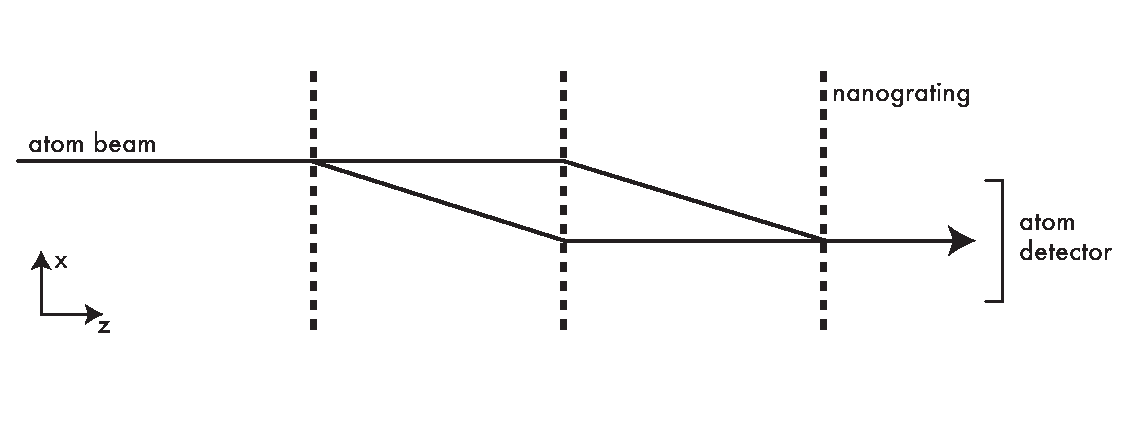
\includegraphics[width=1\textwidth]{Figures/bareIFM.eps}
\caption[A three grating Mach-Zehnder atom interferometer.]{\label{simpleIFM}A three grating Mach-Zehnder atom interferometer. Atoms waves diffracted by the first and second nanogratings form an interference pattern at the third nanograting. A hot-wire detector measures the transmitted atom beam flux.}
\end{figure}


The superposition of traveling waves overlaps at the location of the 3rd nanograting and make a probability of detecting each atom at location $x$ given by
\begin{eqnarray}
|\psi|^2&=&|\psi_0+\psi_1|^2\nonumber\\
&=&A^2+B^2+AB\left(e^{i(k_x x + \delta_\phi)}+e^{-i(k_x x + \delta_\phi)}\right)\nonumber\\
&=&A^2+B^2+2AB\cos(k_x x + \delta_\phi)
\end{eqnarray}
where $\delta_\phi = \phi_1-\phi_0$. The probability density is described by a constant value plus a term that oscillates with a spatial frequency equal to the nanograting period, regardless of the atomic velocity $v=\hbar k_z/m$. As such, we can use a 3rd nanograting as a mask of the interference pattern. The transmitted flux, $I(x)$, can be written in terms of an average beam flux $I_0$, contrast $C$, and phase $\delta_\phi$:
\begin{eqnarray}
I(x)=I_0+C\cos(k_x x + \delta_\phi).
\end{eqnarray}
Moving any of the nanogratings in the $x$ direction scans the atomic interference pattern across the third nanograting to yield intensity vs.~position data. A co-propogating laser interferometer measures the relative position of the three nanogratings. Figure \ref{atomFringe} shows an example of the atom interference fringe data. 


The observed fringe pattern is the incoherent sum of the sinusoidal probability distributions from single-atom interference, repeated about $10^5$ times per second. Different atoms have different velocities and also enter and exit the interferometer at different times. Atoms do not interfere with other atoms in our interferometer, only with themselves, because they are separated from other atoms by tens of micrometers on average. These characteristics are crucial for understanding contrast loss in our interferometer, and in particular the new velocity measurement technique described in section \ref{choppersBrief} and Appendix B. 


Application of, say, an electric field gradient across the interferometer changes $\delta_\phi$ and results in a measurable phase shift. We analyze these phase shifts to determine properties such as atomic polarizability, described in section \ref{polBrief} and Appendix A, and magic-zero wavelengths, described in section \ref{mzwBrief} and Appendix C.


\begin{figure}
\centerline{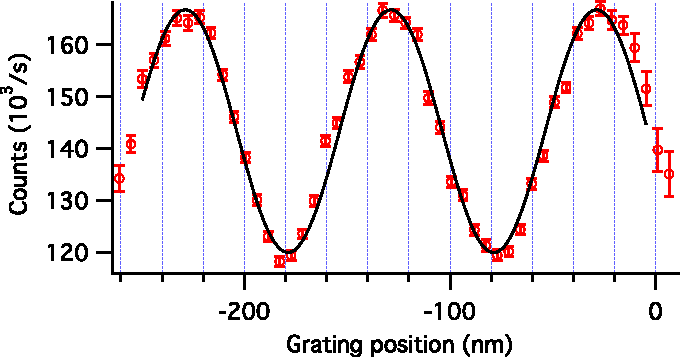
\includegraphics[width=.75\textwidth]{Figures/atomFringe.pdf}}
\caption[Atom interference fringe.]{\label{atomFringe}A typical atom interference fringe from our Mach-Zehnder atom interferometer determined from 5 sec of data. We fit this data to find the fringe contrast $C$ and phase $\phi$.}
\end{figure}


The phase of the atom waves along each path evolve according to
\begin{eqnarray}
\phi=\frac{1}{\hbar} \int E(t) dt
\end{eqnarray}
where $E(t)$ is the total energy of the atom as a function of time. All of the phase shifts described in this thesis are created by energy shifts ($\sim$1 $\mu$eV) much smaller than the kinetic energy of the atoms ($\sim$0.1 eV), and much more slowly varying ($\sim$100 $\mu$m) than the de Broglie wavelength ($\sim$10 pm). These are, loosely, the conditions for the application of the WKB approximation. In the WKB approximation the phase is described by
\begin{eqnarray}
\phi=\frac{1}{\hbar} \int p(z) dz
\end{eqnarray}
where
\begin{eqnarray}
p(z) = \sqrt{2m(E-U(z))}
\end{eqnarray}
is the momentum of the atom. Since $U(z)\ll E$ we can simplify the phase:
\begin{eqnarray}
\phi &=& \frac{\sqrt{2mE}}{\hbar} \int \sqrt{1-\frac{U(z)}{E}} dz \\
	&\approx& \frac{\sqrt{2mE}}{\hbar} \int \left(1-\frac{U(z)}{2E} \right) dz.
\end{eqnarray}
The first term will be common to both paths and not measurable, so we drop it from consideration. The second term corresponds to the change in phase of the wavefunction due to the application of a potential. Finally, plugging in the kinetic energy $mv^2/2$ for the total energy yields a phase shift of
\begin{eqnarray}
\label{phiUx}
\phi=-\frac{1}{\hbar v} \int U(z) dz.
\end{eqnarray}
Typical interaction distances in our experiments are 100 $\mu$m to 10 mm and at a typical atom beam velocity of $v_0=2000$ m/s, this corresponds to interaction times of 50 ns to 5 $\mu$s. As stated previously, the energy shift of a polarizable atom is given by 
\begin{eqnarray}
U(\omega) = -\frac{1}{2} \alpha(\omega) \vec{E}^2(\omega,z,t)
\end{eqnarray}
where we now allow for a frequency dependence for the polarizability and the electric field. Our static polarizability measurements investigate this energy shift in the limit $\omega \rightarrow 0$ and our magic-zero wavelength measurement investigates the frequency at which $\alpha(\omega)$, and thus $U(\omega)$, vanishes.


Depending on the geometry of the interaction region, both paths of the atom interferometer may receive a phase shift. However, we only measure the difference in the phase shifts along two interferometer paths. We refer to this as the differential phase shift. The experiments described in this thesis all apply phase shifts to both paths of the interferometer. Section \ref{polBrief} discusses some of the advantages of this configuration, such as the fact that it enables us to use heavier atoms that produce unresolved diffraction orders.


As discussed above, the measured interference pattern is the ensemble average of single-atom interference patterns. In general, interferometer phase shifts may be a function of many parameters, such as the atom velocity $v$, transverse position $x$, or the atomic state. For example, equation \ref{phiUx} shows that the phase shift is a function of the atom beam velocity. Our supersonic atom beam contains atoms with a narrow, but still significant velocity distribution $P(v)$. Figure \ref{diffractionPofv} shows examples of typical velocity distributions in our interferometer. We use polar notation in the complex plane to more easily and compactly express and calculate the ensemble average of interference fringes. For the case of averaging over only a velocity distribution the expression is
\begin{eqnarray}
\label{cmphim}
C_m e^{i\phi_m}=C_0 e^{i\phi_0} \int_{v=0}^\infty P(v)e^{i\phi(v)}dv
\end{eqnarray}
where $\phi(v)$ is the velocity-dependent differential phase shift, $C_m$ are $\phi_m$ are the measured interferometer contrast and phase, respectively, and $C_0$ are $\phi_0$ are the interferometer phase and contrast in the absence of the phase shift. We typically evaluate equations such as \ref{cmphim} by numerical integration of the real and imaginary parts of the right side of the equation. Then, $C_m$ is given by the magnitude of the complex number on the right side of the equation, and $\phi_m$ is given by the polar angle. In the limit that $P(v)\rightarrow\delta(v-v_0)$ we obtain $\phi_m=\phi_0+\phi(v_0)$ and $C_m=C_0$, as expected. Additional parameters, such as the transverse beam position, may be averaged over in a similar fashion. The distribution of phase shifts associated with these parameters typically leads to contrast loss in the interferometer. 


\begin{figure}
\centerline{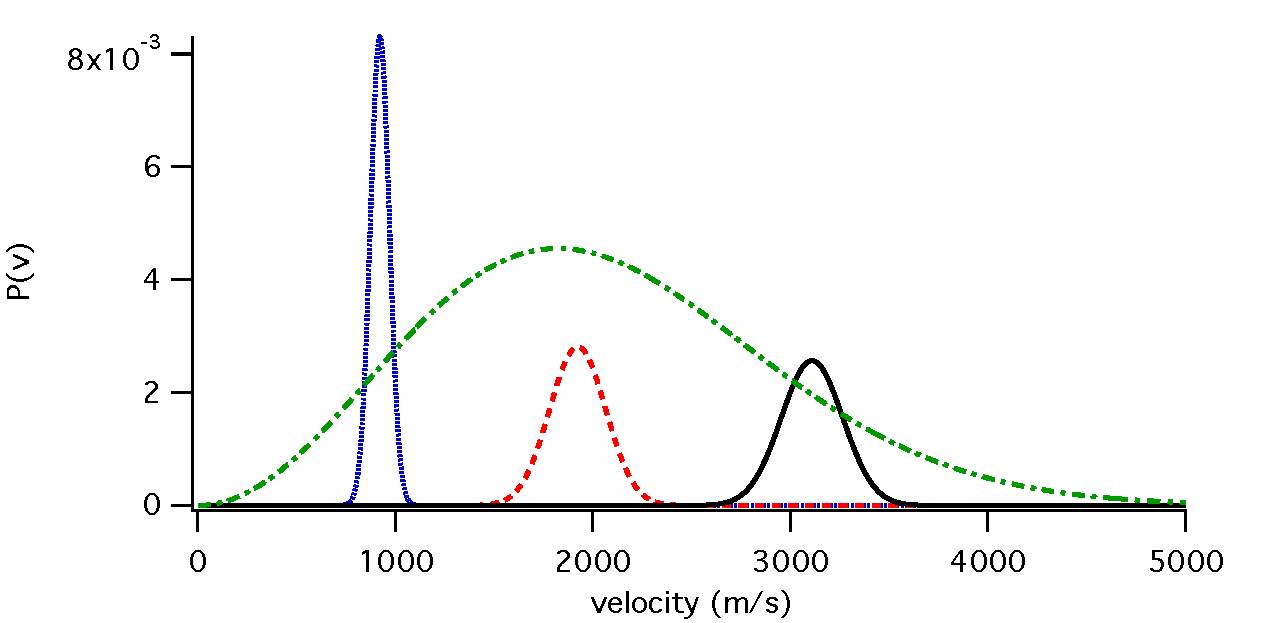
\includegraphics[width=1.0\textwidth]{Figures/diffractionPofv2.pdf}}
\caption[Probability distribution of velocities in supersonic atom beams.]{\label{diffractionPofv} Probability distribution of velocities for supersonic beams of Rb (blue dotted), K (red dashed), and Na (black solid), as measured in Figure \ref{nakrbDiffraction}. Each distribution is normalized such that $\int_0^\infty P(v) dv =1$. For comparison, we also show the velocity distribution of a Maxwell-Boltzmann gas of He atoms at 800 K (green dot-dashed) that is used as the carrier gas for the Na supersonic beam, normalized to 10 for visibility.}
\end{figure}







\chapter{THIS THESIS IN BRIEF}

This chapter explains the essential components of the three experiments that make up the majority of this thesis work: First, a measurement of the static polarizabilities of sodium, potassium, and rubidium (section \ref{polBrief}). Next, a novel and more precise method to measure the velocity of atom beams (section \ref{choppersBrief}) that will improve future polarizability measurements. Then, a measurement of a wavelength of light at which the dynamic polarizability of potassium is zero, known as magic-zero wavelength (section \ref{mzwBrief}). This chapter also contains summaries of a proposal to measure the polarizability of strontium using a photoionization detector, and a proposal to measure the tensor polarizabilities of alkali dimers.



%%%%%%%%%%%%%%%%%%%%%%%%%%%%%%%%%%%
\pagebreak
\section{Static polarizability measurements of Na, K, and Rb}
\label{polBrief}

In 2008, we set out to establish a new atomic polarizability measurement program in Arizona. In 2010 we published the first improved measurements of potassium and rubidium polarizability in over 35 years \cite{Hol10}. The paper, published in \emph{Physical Review A}, is included in Appendix \ref{polPRAappendix}. Chapter \ref{polChapter} explains additional details of this experiment. Section \ref{introPolHistory} reviewed the history of polarizability measurements and Figure \ref{polPreviousWorkPlot} summarizes previous calculations and measurements of alkali polarizabilities.

We measured the polarizabilities of sodium, potassium, and rubidium using a Mach-Zehnder atom interferometer with an interaction region containing an electric-field gradient. The interferometer and electrodes are shown in Figures \ref{ifm2010pra} and \ref{int2010photo}. We measured each polarizability (for Na, K, and Rb) independently, and we refer to these as absolute measurements. We also reported ratios of polarizabilities, since we can do this with even higher precision. Table \ref{polResultsTable} shows the absolute measurements (less than 1.0\% uncertainty), and Table \ref{polRatiosTable} shows the ratio measurements (0.3\% precision). 

Our measurements of polarizability ratios are new in atom interferometry, and are possible because nanogratings diffract all types of atoms and molecules. Although this unique feature of our interferometer has long been recognized, the work described in this thesis is the first time that the utility of nanogratings for multiple species has actually been used for a precision measurement of polarizability. The benefit of presenting ratios is that systematic errors are nearly the same for different atomic species and cancel when determining polarizability ratios. We combined our ratio measurements with the higher-precision measurement of sodium polarizability by Ekstrom \etal \cite{Eks95} to present the most precise measurements of potassium and rubidium polarizability currently available. Our measurements were recently included in an updated table of polarizabilities in the CRC Handbook of Chemistry and Physics \cite{Mil12}.


\begin{figure}
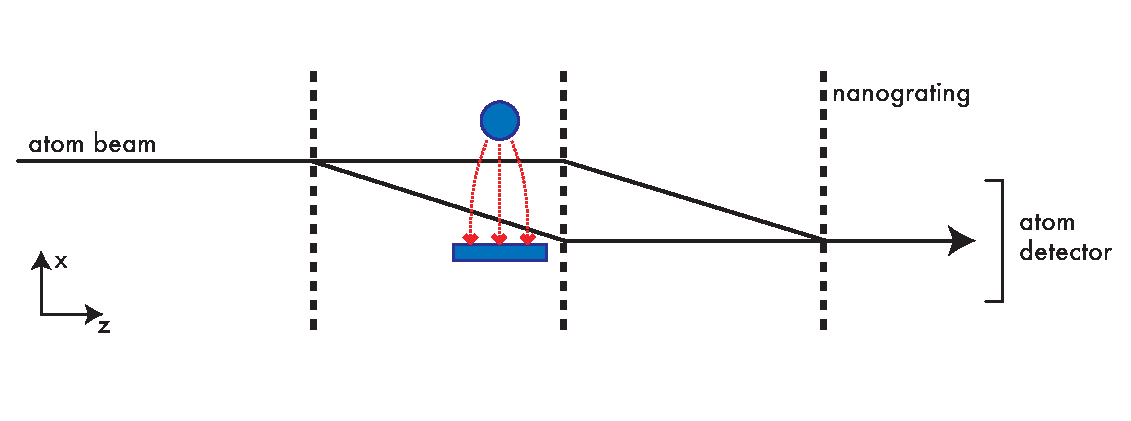
\includegraphics[width=1\textwidth]{Figures/ifmWith2010pol.eps}
\caption[Interferometer with polarizability measurement electrodes.]{\label{ifm2010pra} Atom interferometer with electric field gradient region (blue electrodes, red field lines) to measure static polarizabilities. An atom passing through the interaction region acquires a phase shift along each path and we measure the differential phase shift.}
\end{figure}


\begin{figure}
\centerline{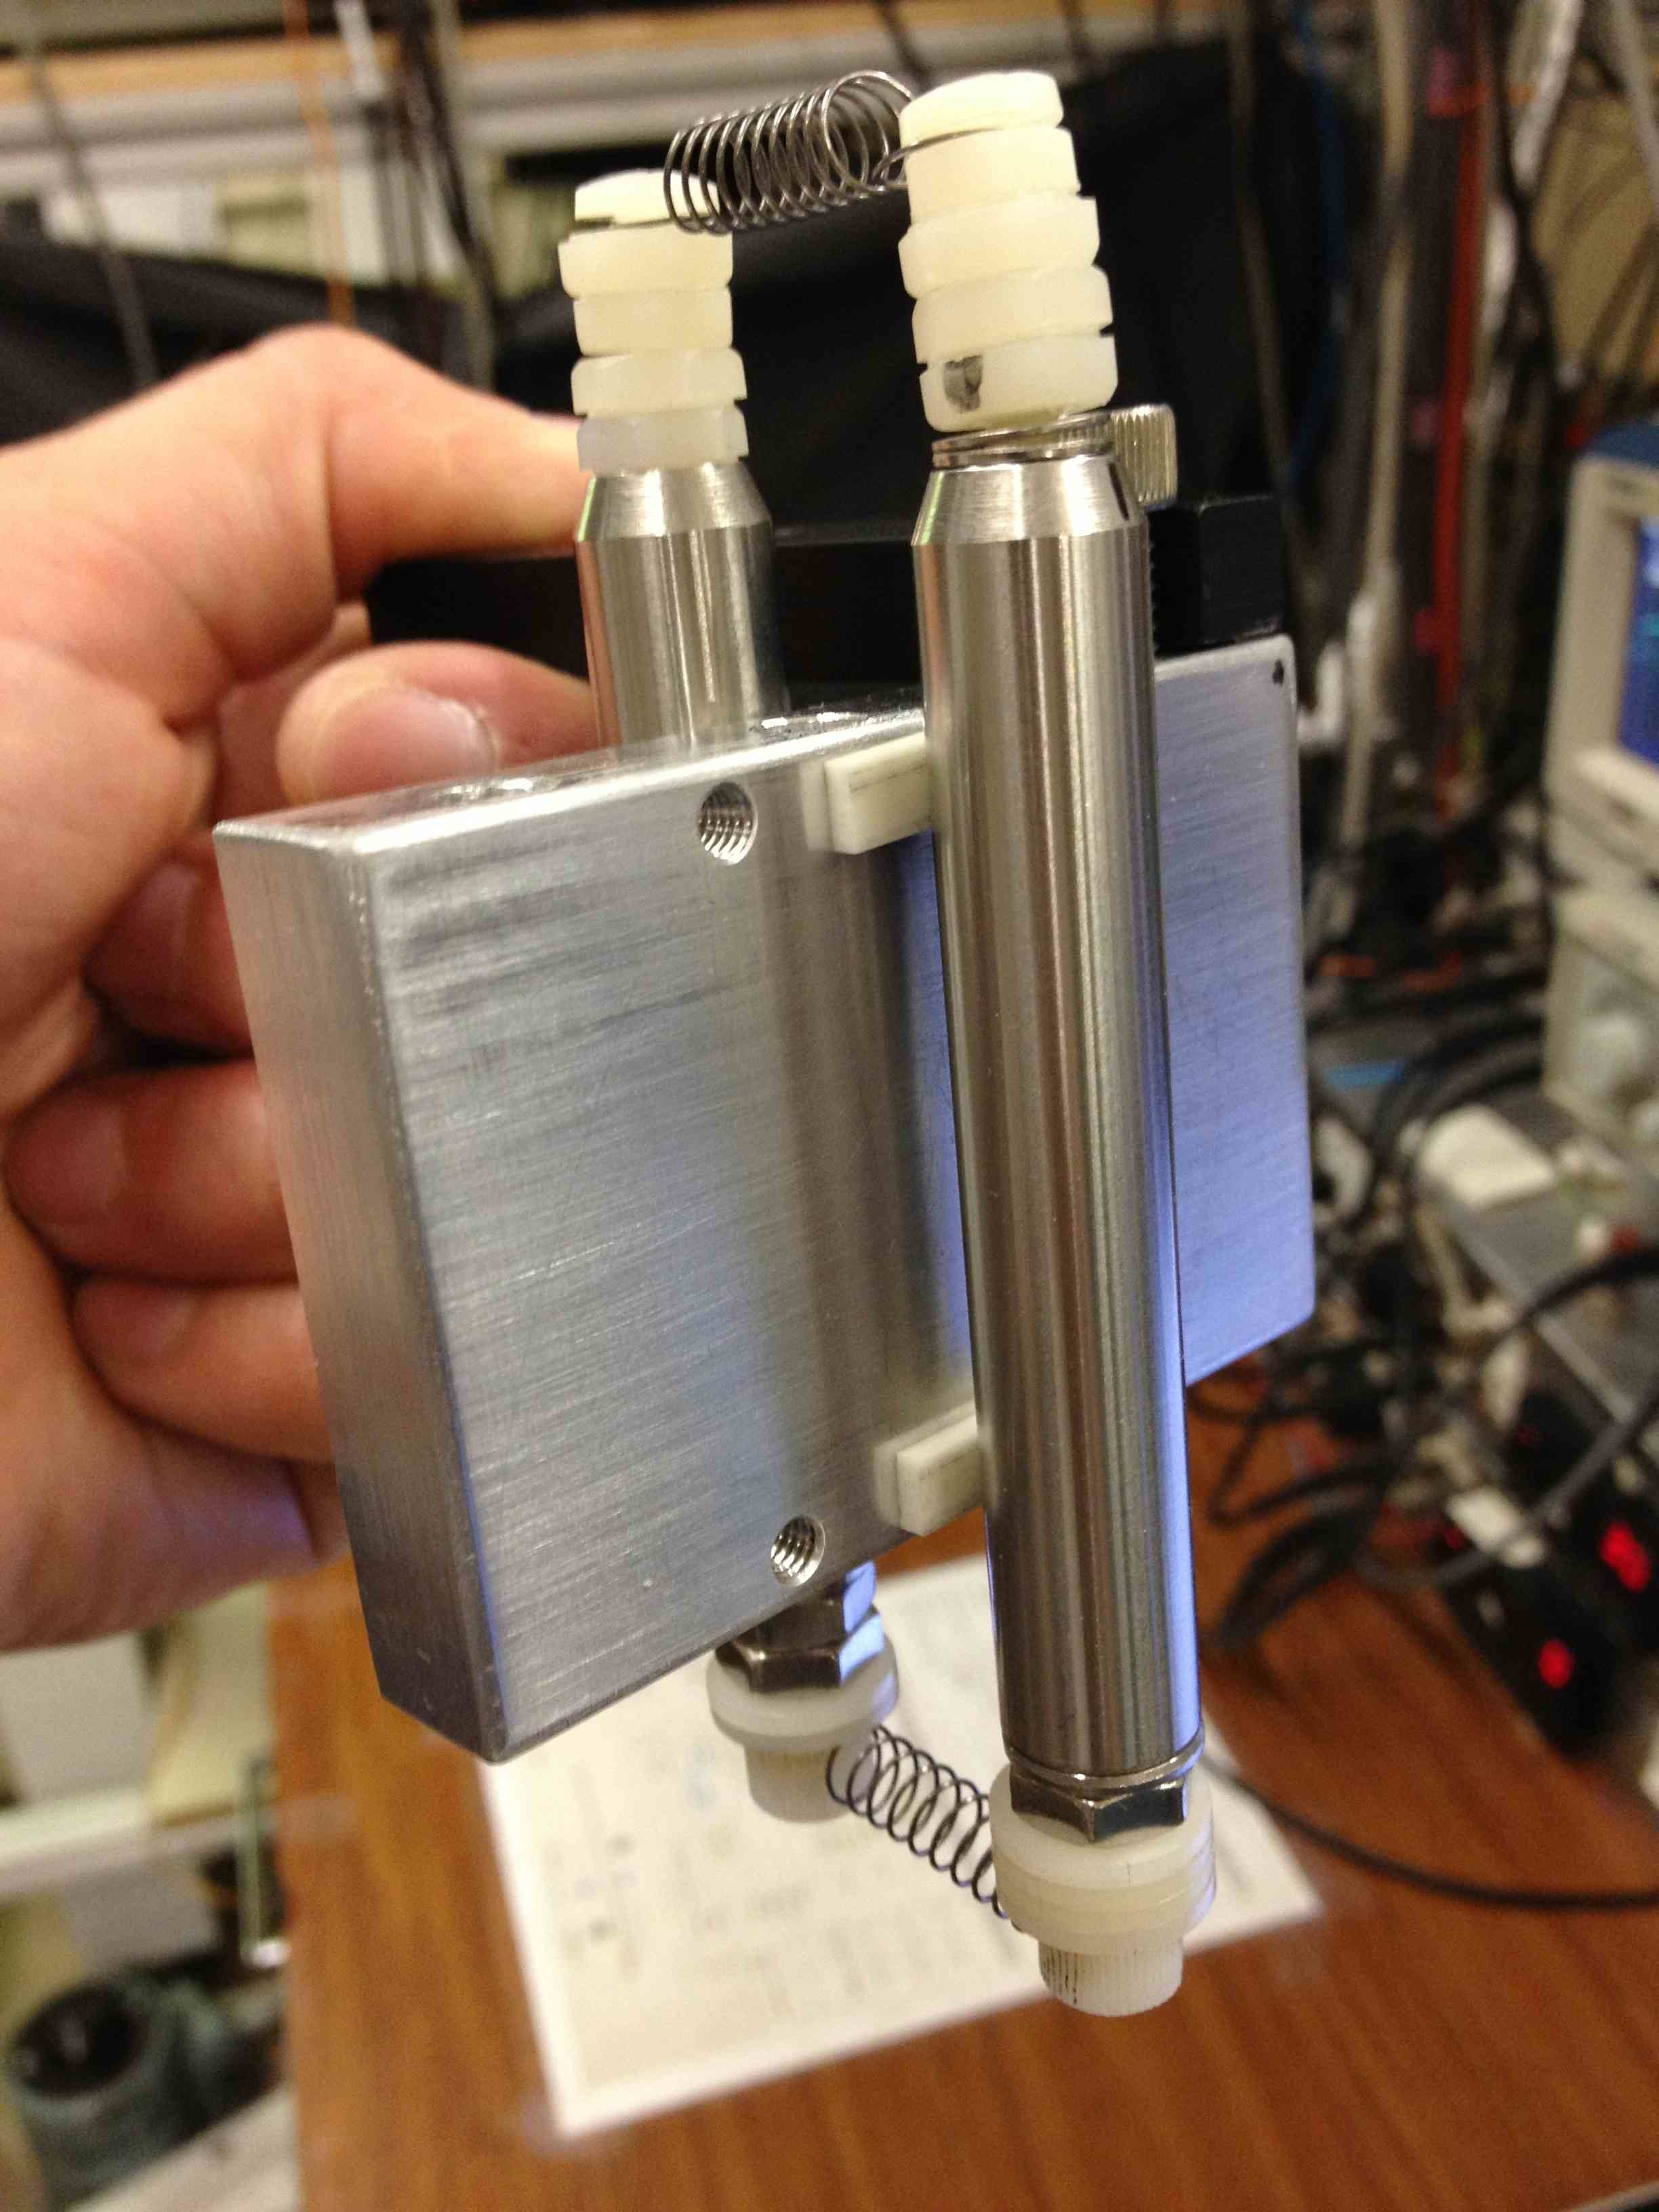
\includegraphics[width=.40\textwidth]{Figures/intRegion2010photoCompMore.jpg}}
\caption[Photograph of the 2010 polarizability measurement electrodes.]{\label{int2010photo}Photograph of the polarizability measurement electrodes. The atom interferometer paths pass through electric-field gradient between the rectangular ground plane and the cylindrical electrode.}
\end{figure}


\begin{table}
\caption[2010 PRA measurements of atomic polarizabilities.]{\label{polResultsTable}Measured absolute and recommended atomic polarizabilities in units of $10^{-24}\textrm{ cm}^3$.  Our recommended polarizability values are based on our ratio measurements (see Table \ref{polRatiosTable}) combined with the sodium polarizability measurement from Ekstrom \etal \cite{Eks95}.}
\begin{center}
\begin{tabular}{c c c c}
\hline\hline
& $\alpha_\textrm{abs}$(stat.)(sys.)  & { $\textrm{  }$ $\textrm{  }$ } & $\alpha_{\textrm{rec}}$(tot.)\\
\hline
Na & 24.11(2)(18) & & 24.11(8)\\
K & 43.06(14)(33) & & 43.06(21)\\
Rb & 47.24(12)(42) &  & 47.24(21)\\
\hline
\end{tabular}
\end{center}
\end{table}



\begin{table}
\caption[2010 PRA measurements of atomic polarizability ratios.]{\label{polRatiosTable}Measured atomic polarizability ratios with statistical uncertainties. Also included are several polarizability ratios from \emph{ab initio} and semi-empirical calculations. See Fig.~\ref{polPreviousWorkPlot} for more calculations and measurements of polarizability ratios.}
\begin{center}
\begin{tabular}{c | c | c c c}
\hline\hline
 &  $\alpha_\textrm{ratio}$(stat.~unc.) & & Theory\\
Atoms & This work & Ref \cite{Der99} & Ref \cite{Saf99} & Ref \cite{Mit03} \\
\hline
Rb/Na & 1.959(5) & 1.959(5) & 1.946 & 1.939 \\
K/Na    & 1.786(6) & 1.785(6) & 1.779 & 1.781 \\
Rb/K    & 1.097(5) & 1.098(5) & 1.094 & 1.089 \\
\hline\hline
\end{tabular}
\end{center}
\end{table}



\begin{figure}
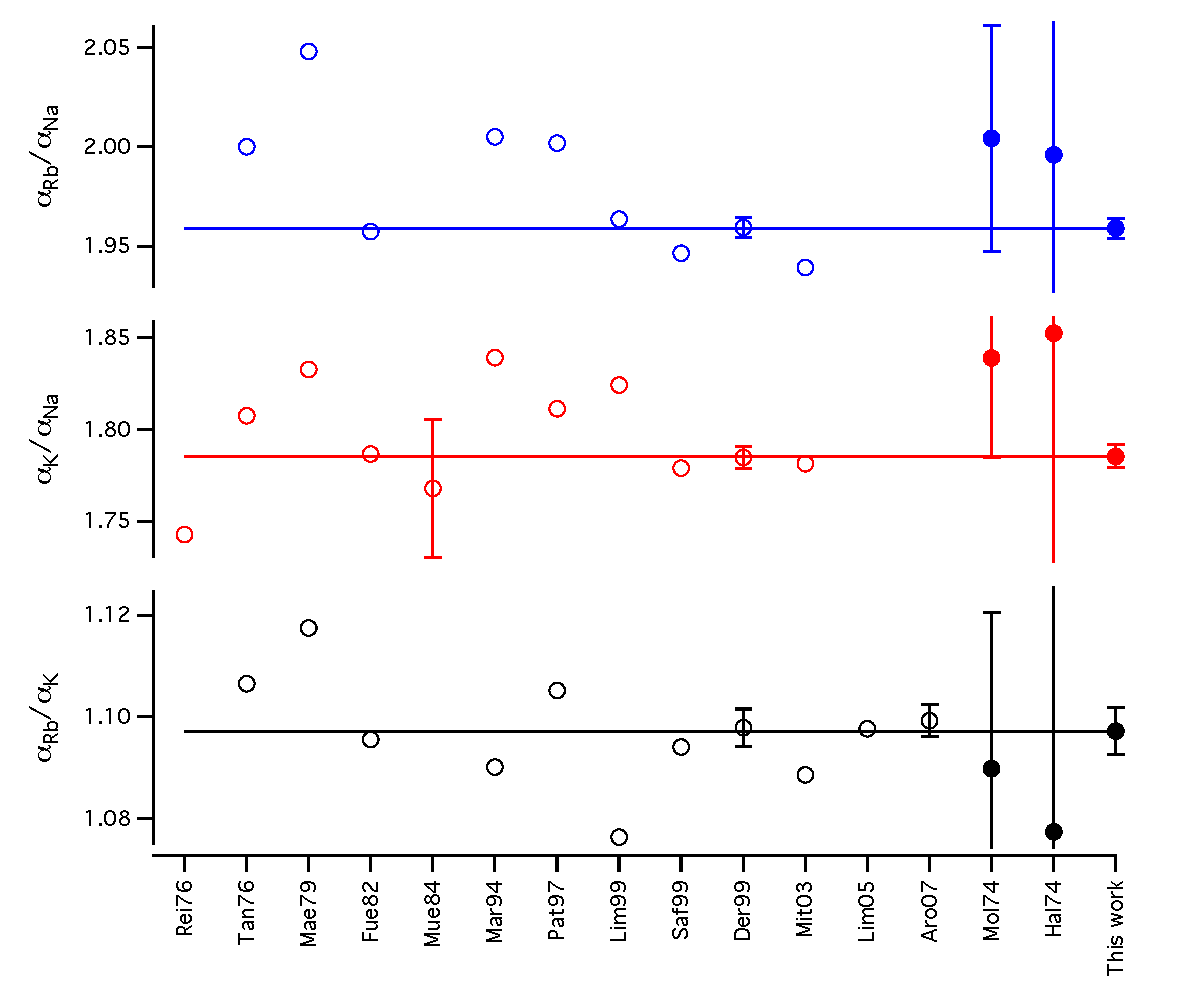
\includegraphics[width=1\textwidth]{Figures/PolPRAratios.pdf}
\caption[Previously calculated and measured alkali polarizability ratios.]{\label{polPreviousWorkPlot} Previously calculated (unfilled) and measured (filled) alkali polarizability ratios. References are denoted by the abbreviated first author's name and the publication year. Calculations in references Derevianko \etal (1999) \cite{Der99} and Arora \etal (2007) \cite{Aro07} incorporate state lifetime measurements.}
\end{figure}



Another unique feature of this work compared to other atom interferometry measurements of polarizability \cite{Eks95,Mif06} is that we use an electric-field gradient region to apply phase shifts to both paths rather than a septum electrode, which would apply a phase shift to only one path. Electric-field gradient regions have the advantage of not requiring an electrode to be placed between the two atom beam paths. This allows us to study heavier atoms with shorter de Broglie wavelengths and therefore smaller path separations. Since the electric-field gradient interaction region does not require resolved diffraction orders, another advantage is that we can use a less collimated beam to increase the flux and reduce the systematic error caused by velocity-selective detection of atoms in the interferometer. However, electric-field gradient regions have the disadvantage that the measured differential phase shift is proportional to $1/v^2$, rather than $1/v$, so the uncertainty in beam velocity measurements contributes twice as much to uncertainty in polarizability measurements. The phase shift in an electric-field gradient region also depends sensitively on the location of the atom beam paths with respect to the electrodes, unlike in a septum geometry with a uniform electric field. 


\begin{figure}
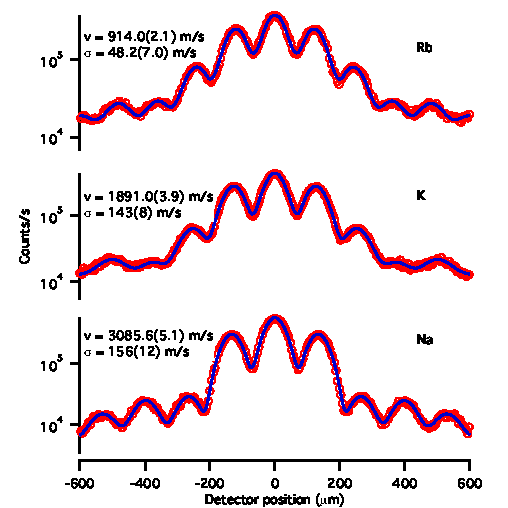
\includegraphics[width=1\textwidth]{Figures/Fig3Diffraction2.pdf}
\caption[Diffraction of Na, K, and Rb.]{\label{nakrbDiffraction} Diffraction of Na, K, and Rb atoms determines the average velocity, $v_0$, and the velocity distribution width, $\sigma_v$, of the atom beams. Figure \ref{diffractionPofv} shows the velocity distributions determined by these measurements.}
\end{figure}



The primary limitation of the absolute polarizability measurements in this experiment was determining the velocity and velocity distribution of the atom beam. We determined the atom beam velocity by studying atomic diffraction patterns in the far-field of the first nanograting, such as those shown in Figure \ref{nakrbDiffraction}. The atom beam velocity is given by rewriting equation \ref{sepEqn} as
\begin{eqnarray}
v(x_n)=\frac{z_{det}hn}{md_gx_n}
\end{eqnarray}
where $z_{det}$ is the distance from the first nanograting to the detector, and $x_n$ is the position of the $n$th diffraction order. In reality, a distribution of velocities exists in the supersonic atom beam, and this leads to a distribution of diffraction patterns. The velocity distribution can be well described by a Gaussian with an average velocity $v_0$ and width $\sigma_v$. Figure \ref{diffractionPofv} shows examples of typical supersonic atom beam velocity distributions. To better compare velocity distributions with different average velocities, it is useful to define a sharpness ratio $r=v_0/\sigma_v$. 




Each observed diffraction pattern is a convolution of the atom beam profile, the detector width, and the atom beam velocity distribution. Figure \ref{diffractionConv} illustrates the individual features that lead to the observed diffraction patterns. Uncertainties in $z_{det}$, the detector translation angle, and the details of this convolution limited the accuracy of the velocity measurement to 0.3\%, and thus contributed 0.6\% uncertainty to the absolute polarizability measurements. 


\begin{figure}
\centerline{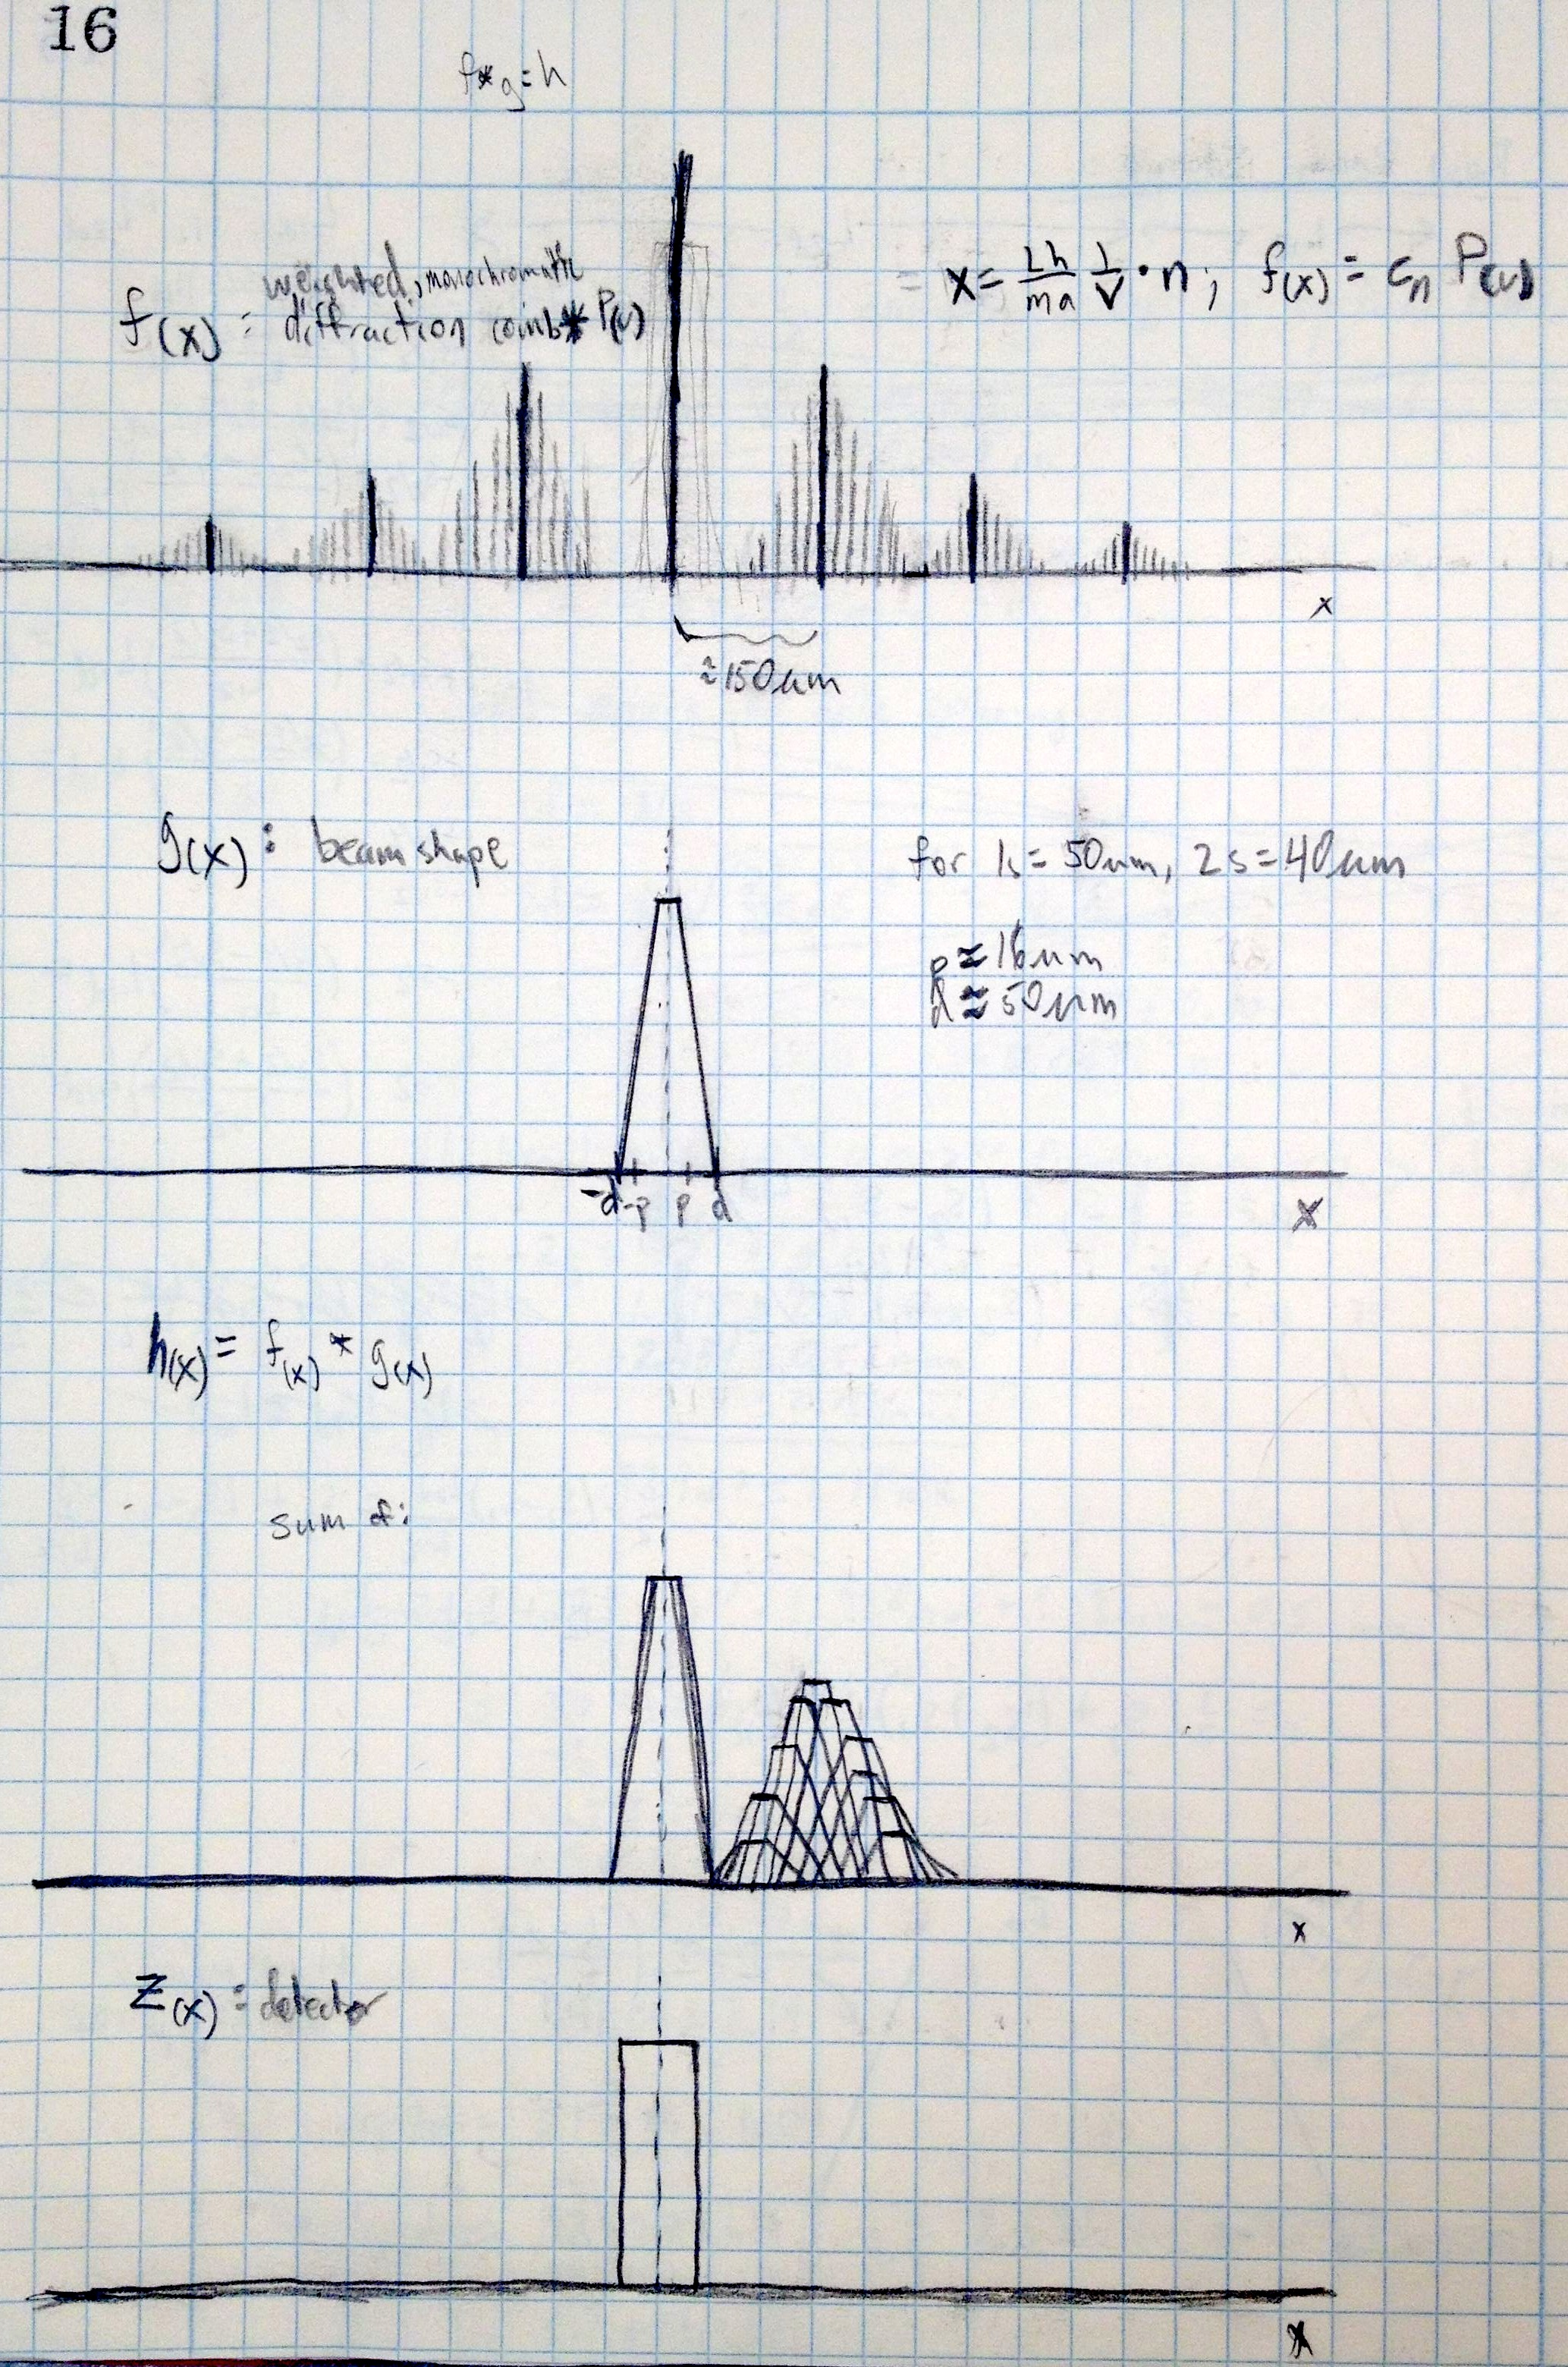
\includegraphics[width=.75\textwidth]{Figures/diffractionConvolution4.jpg}}
\caption[Convolution of atom beam profile, detector width, and velocity distribution for diffraction patterns.]{\label{diffractionConv} From top to bottom the plots show: the diffraction comb for different velocity classes, the trapezoidal atom beam profile obtained using two collimating slits, the convolution of the beam profile with the velocity distribution, and the hot-wire detector size. Figure from Will Holmgren lab notebook number 1 (June 2008).}
\end{figure}



If we ignore smaller effects such as the velocity distribution and the atom beam thickness (treated in detail in Appendix A), we can obtain a simple expression for the measured polarizability:
\begin{eqnarray}
\label{simplePol}
\alpha \approx \frac{v^2}{kV^2x_\textrm{int}}\phi_\alpha.
\end{eqnarray}
Here, $k$ is a constant that depends on the geometry of the interaction region, $V$ is the voltage applied to the interaction region, and $x_\textrm{int}$ is the transverse position of the interaction region. Figure \ref{phasePosition2010} shows a plot of the phase shift as a function of the interaction region position.

\begin{figure}
\centerline{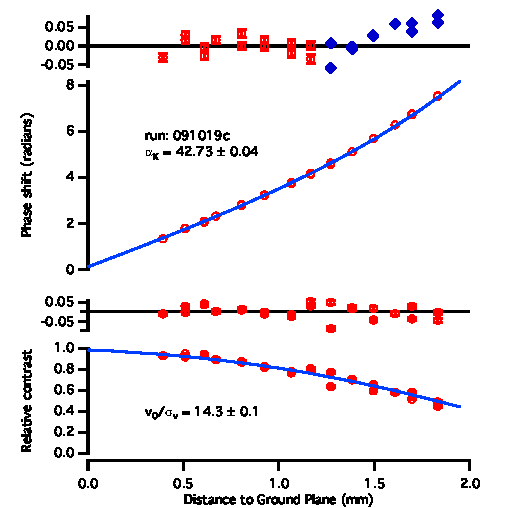
\includegraphics[width=0.75\textwidth]{Figures/Fig4PhaseFit.pdf}}
\caption[Phase shift and contrast vs.~interaction region position.]{\label{phasePosition2010} Interferometer phase shift and relative contrast vs.~interaction region position. We fit the phase shift data to determine the atomic polarizability. Higher phase shift data (blue points) was excluded from the fit due to their higher sensitivity to uncertainties in the velocity distribution width.}
\end{figure}

To measure the atom beam position $x_\textrm{int}$, we blocked the atom beam with the high voltage electrode and then moved the electrodes until the atom beam was visible again. Analysis of the transmitted flux vs.~electrode position allowed us to determine the atom beam position with a precision of 1 $\mu$m. We refer to this as the eclipse method. Unfortunately, we later determined that the motor position report was not as reliable as desired, and contributed a random error to the polarizability measurements. For the electrodes used in this experiment, a 10 $\mu$m error in beam position caused a 1\% error in the polarizability measurement. We now believe that 5-10 $\mu$m position errors were likely for each of the phase measurements, and this led to additional random error in the polarizability measurements. See section \ref{polChapterGradElg} for more details.


All systematic sources of error, such as uncertainty in $z_{det}$, the interaction region geometry, or the electrode voltages, are nearly identical for each atomic species. At the level of precision of our experiment, these systematic uncertainties cancel when presenting ratio measurements of polarizabilities. We measured the polarizability of each atomic species between 13 and 23 times (see Figure \ref{polPRAmeasurementsTrim}) and the reproducibility of the measurements determines the statistical uncertainty. The reported statistical uncertainty is the standard error of the mean. The irreproducibility of the data was larger than we expected given the interferometer contrast and count rate, primarily due to the faulty electrode position measurements.  


To improve upon our 2010 polarizability measurements, we developed a next-generation static polarizability experiment to reduce most uncertainties associated with this experiment. We developed a new velocity measurement technique (described in the next section), changed the geometry of the electric-field gradient region, improved the electrode position measurement, improved a number of distance measurements, and developed a new data acquisition system. Sections \ref{newDAQ} and \ref{polChapterGradElg} and Chapter \ref{choppersChapter} discuss the improved system in more detail.





%%%%%%%%%%%%%%%%%%%%%%%%%%%%%%%%%%%%%%%
\pagebreak
\section{Phase choppers: a new atom beam velocity measurement technique}
\label{choppersBrief}

Atom beam velocity was the largest source of uncertainty in our 2010 polarizability measurements. To reduce this uncertainty we developed a new technique to measure atom beam velocity called \emph{phase choppers} \cite{Hol11}. Phase choppers provide a more precise and more accurate measurement of beam velocity than can be obtained with diffraction. Chapter \ref{choppersChapter}, Appendix \ref{choppersAppendix}, and C.E. Klauss' B.S.~thesis \cite{Kla11} describe this technique in detail. Phase choppers are similar to the phase shifters described in \cite{Rob04} and their utility for measuring beam velocity was first proposed in \cite{Rob02}. Here, we summarize the most important features.

Phase choppers have numerous advantages over atom beam diffraction and other velocity measurement techniques:
\begin{enumerate}
\item Higher precision measurements in less time
\item Frequency-based instead of length-based measurement
\item No need for well-separated diffraction orders, so choppers can be used with faster beams (higher flux) and more massive atomic species
\item \emph{in situ} measurement of velocity distribution of atoms contributing to the interference fringes
\item No moving parts
\end{enumerate}

To understand how phase choppers can measure atom beam velocity, it helps to first consider mechanical choppers. Two spinning mechanical choppers (slotted disks) separated by a distance $L$ and blocking the beam at frequency $f$ can transmit atoms with velocity $v = nLf$, where $n$ is an integer. An atom with velocity $v$ will travel a distance $L$ from the first chopper to the second chopper in a time $\tau=L/v$, corresponding to a fundamental chopping frequency $f_0=v/L$. 

Mechanical choppers simply block or transmit atoms, leading to a maximum in the transmitted flux when the chopping frequency is any integer multiple of $f_0$. In the method we present here, phase choppers are switched on and off by a function generator to periodically apply phase shifts to atomic de Broglie waves in an interferometer. This leads to a maximum in the interferometer \emph{contrast}, instead of the \emph{flux}, when the chopping frequency satisfies $f=n f_0$. The ability to control wavefunction phase, rather than amplitude, provides a more featured and higher flux data set and allows for a more precise determination of velocity. 


\begin{figure}
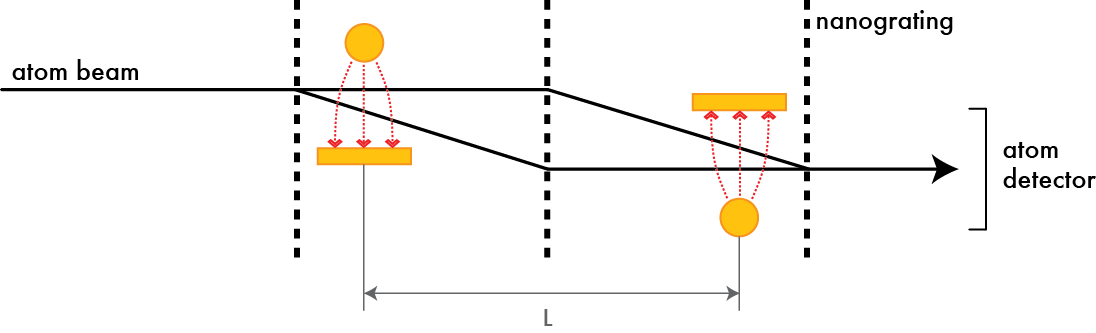
\includegraphics[width=1\textwidth]{Figures/IFMwithChoppers.png}
\caption[Phase choppers in the atom interferometer.]{\label{choppersIFMsimple}Two phase choppers are placed in the interferometer at a distance $L = 1270.68(25)$ mm apart. A square-wave voltage $V(t)$ applied across the choppers creates an electric field (dashed lines). Atoms with velocity $v$ passing through chopper 1 and chopper 2 acquire net differential phase shifts $\phi_1(t)+\phi_2(t+L/v)$.}
\end{figure}


Figure \ref{choppersIFMsimple} shows two phase choppers added to the atom interferometer. Before continuing, it is worth restating an important principle regarding how our atom interferometer works: the observed fringe pattern is the incoherent sum of the sinusoidal probability distributions from single-atom interference, repeated about $10^5$ times per second. Different atoms have different velocities and enter and exit the interferometer at different times. We observe an ``average" of all of these fringe patterns. Therefore, if half of the atoms receive phase shifts that are $\pi$ different from the other half of the atoms, then the measured interference contrast $C$ will be 0. Mathematically, we would observe an intensity $I=I_0 + C_0(0.5\sin(k_x x)+0.5\sin(k_x x+\pi))=I_0+C\sin(k_x x)$ with $C=0$. 

\begin{figure}
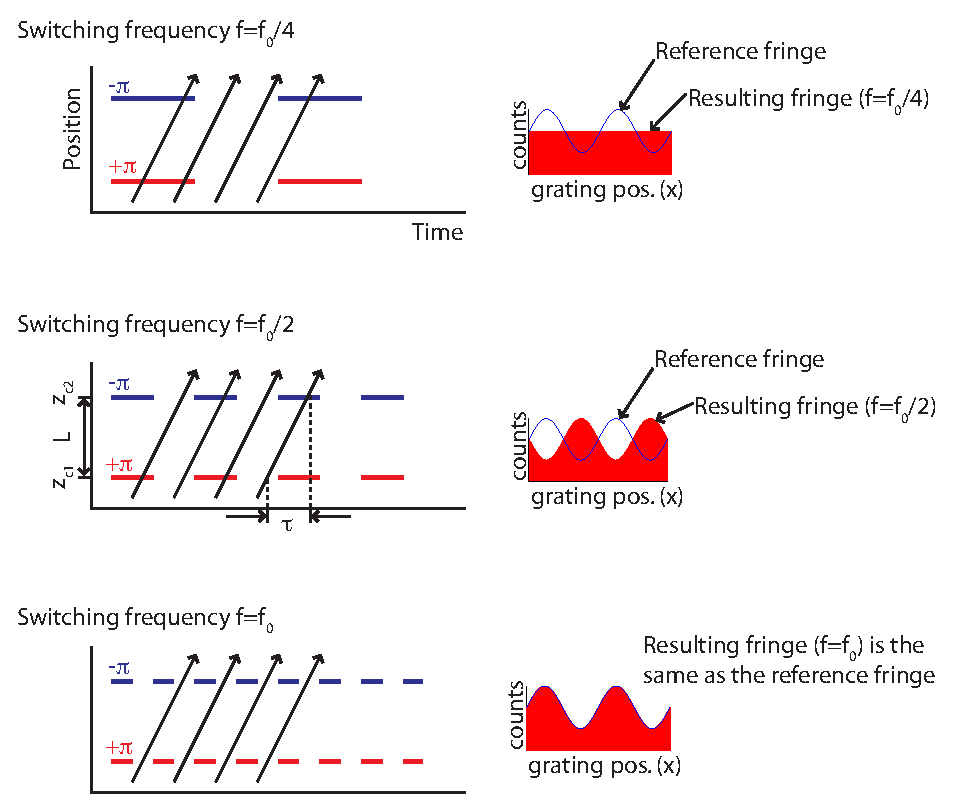
\includegraphics[width=1\textwidth]{Figures/PhaseChoppersVvst4.eps}
\caption[Interferometer contrast for particular chopping frequencies.]{\label{VvsT}Atoms with different starting times will acquire 0, $+\pi$ (red), or $-\pi$ (blue) phase shifts as they pass through chopper 1 and chopper 2, depending on their velocity $v$ and the chopping frequency $f$. The time it takes an atom with velocity $v$ to travel the distance $L$ between the choppers is $\tau$ and $f_0=1/\tau$. We measure the average of the sinusoidal probability distributions formed by each atom interfering with itself, shown at right. The reference interference pattern with the choppers off is shown in blue and the resulting interference patterns with the choppers on are shown in red.}
\end{figure}

Depending on its start time, velocity, and the chopping frequency, an atom will pass through the two choppers in one of four possible pairs of conditions (off-off, on-off, off-on, or on-on). We now describe what happens to the interference pattern created by atoms with a single velocity $v$ when the choppers are switched at four particular frequencies (see Figure \ref{VvsT}):
\begin{itemize}
\item $\bm{f \ll f}\bm{_0}.$ Atoms experience the off-off (0 net differential phase shift) or on-on (0 net differential phase shift) pairs of conditions with equal likelihood, and all atoms emerge with 0 net phase shift. The contrast and phase of the detected ensemble remain unchanged.

\item $\bm{f=f}\bm{_0/4}$. Atoms experience each of the four possible pairs of conditions, off-off (0), on-off ($\pi$), off-on (-$\pi$), or on-on (0), with equal likelihood. Therefore, half of the ensemble will acquire 0 net differential phase shift, and half will acquire a $\pi$ net differential phase shift. The ensemble contrast is 0 and phase is indeterminate. Contrast minima repeat at frequencies $f=(2n+1)f_0/4$, where $n$ is an integer. 

\item $\bm{f=f}\bm{_0/2}$. Atoms experience on-off ($\pi$) or off-on ($-\pi$) pairs of conditions with equal likelihood. The ensemble contrast remains unchanged, but the phase shifts by $\pi$ (modulo $2\pi$). Contrast revivals with $\pi$ phase shifts repeat at frequencies $f=(2n+1)f_0/2$. 

\item $\bm{f=f}\bm{_0}$. Once again, all atoms experience the off-off (0) or on-on (0) states. The ensemble contrast and phase remain unchanged. Contrast revivals with no phase shift repeat at frequencies $f=nf_0$.
\end{itemize}

These simple cases show how by finding the value of $f_0$ one can find the velocity of an atom beam through the relation $v=Lf_0$. The contrast revivals and minima that occur at large $n$ provide a way of leveraging small changes in velocity into large changes in revival and minima frequency. In practice, we find the velocity of our atom beam by measuring the contrast at many frequencies and fitting the contrast data to a model discussed in Appendix B. Figure \ref{CsSimpleChopperScan} shows fitted data from a typical chopper frequency scan using this model. The major corrections to the simple model include methods to account for velocity distribution, velocity dependent phase shifts from the choppers, application of non-$\pi$ average phase shifts, and velocity-dependent phase shifts due to the Sagnac effect.


\begin{figure}
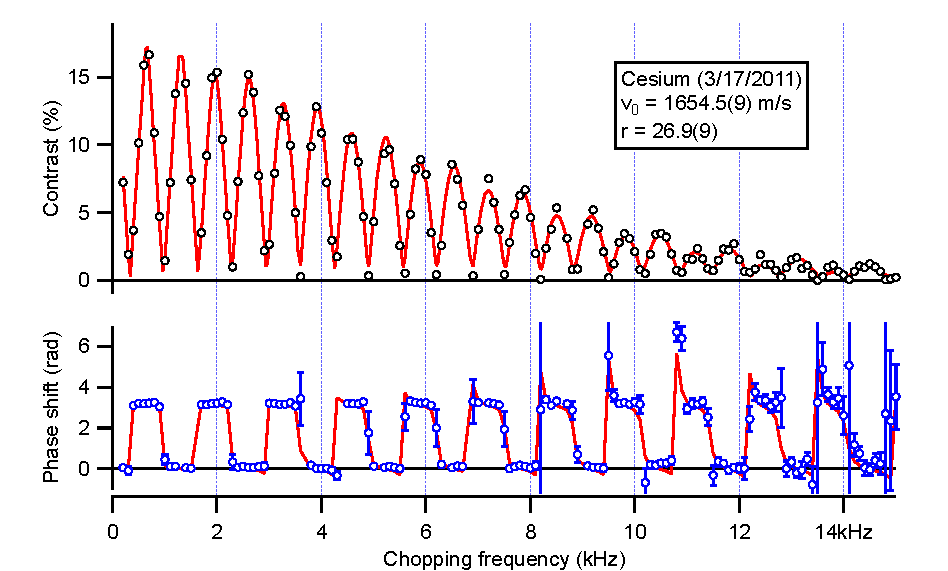
\includegraphics[width=1\textwidth]{Figures/CsSimpleChopperScan.pdf}
\caption[Phase chopper data and best-fit functions.]{\label{CsSimpleChopperScan}Phase chopper data (circles) and corresponding best-fit functions (red curves) for a cesium atom beam with a 70\% helium, 30\% argon carrier gas. We fit the contrast (black) to find the flow velocity $v_0$ and velocity ratio $r=v_0/\sigma_v$. The measured phase (blue) is also shown, but is not fit. Each point is derived from 5 seconds of data. Note that the asymmetric slope of the phase data is due to the Coriolis deflection (Sagnac phase shift).}
\end{figure} 


We also tested the phase choppers by measuring the polarizability of cesium using beams with three very different flow velocities on three different days. Each day we alternated between measurements of beam velocity and polarizability every hour to account for small changes in velocity ($<0.5\%$) over the course of a day due to instability in the beam source temperature. The statistical error of each measurement of velocity was less than 0.1\%. We found the cesium polarizability (stat.~unc.) to be 59.84(4), 59.71(7) and 59.85(8) $\mathrm{\AA}^3$ at flow velocities of 925, 1345 and 1680 m/s. This data is shown in Figure \ref{csPolVelDiff}. These polarizability measurements are subject to a systematic correction due to a revised measurement of the interaction region geometry, but the consistency of the polarizability measurements provides strong evidence that our velocity measurements using phase choppers are reproducible at the 0.1\% level, similar to the measurement of Amini and Gould \cite{Ami03}.







%%%%%%%%%%%%%%%%%%%%%%%%%%%%%%%%%%%%%%%%%
\pagebreak
\section{Measurement of a magic-zero wavelength}
\label{mzwBrief}

Most measurements of static and dynamic polarizabilities are limited by uncertainty in the electric field strength and uncertainty in the time an atom interacts with the field. To avoid these limitations, we designed an experiment to measure the wavelength at which the dynamic polarizability of an atom goes to zero. This is known as the \emph{magic-zero wavelength}, or \emph{tune-out wavelength}. We published our measurement in \emph{Physical Review Letters} \cite{Hol12a} (Appendix \ref{mzwAppendix}) and Chapter \ref{mzwChapter} includes supporting material for this experiment.


A magic-zero wavelength ($\lambdaZero$) occurs between atomic resonances, where the light is red-detuned from one resonance and blue-detuned from another. Opposing contributions from these resonances produce a root in the dynamic polarizability at $\lambdaZero$ and so the energy shift of an atom vanishes at $\lambdaZero$. Figure \ref{KredBlueMZWfig} shows the dynamic polarizability in the vicinity of the four lowest energy transitions of potassium. Three magic-zero wavelengths occur between these four transitions.


Magic-zero wavelengths are understandable in terms of the Lorentz oscillator model of an atom. The equation of motion for an electron in the Lorentz oscillator model yields
\begin{eqnarray}
x(t)=-\frac{e}{m}\frac{1}{\omega_0^2-\omega^2-i\omega\gamma}E(t)
\end{eqnarray}
where $e$ is the electron charge, $m$ is the electron mass, $\omega_0$ is the resonance frequency of the atom, $\omega$ is the frequency of oscillation of the electric field $E(t)$, and $\gamma$ is the damping parameter. We can define a complex polarizability $\alpha(\omega)$ in terms of the dipole moment $p(t)$:
\begin{eqnarray}
p(t)=-ex(t)=\alpha(\omega) E(t)\\
\alpha(\omega)=\frac{e^2}{m}\frac{\omega_0^2-\omega^2+i\omega\gamma}{(\omega_0^2-\omega^2)^2+(\omega\gamma)^2}.
\end{eqnarray}
The real part of the complex polarizability gives the dispersion and the imaginary part corresponds to absorption of light. Magic-zero wavelengths occur far from resonance, where the absorption probability is low and $|\omega_0-\omega|\gg\gamma$, so we drop the imaginary component:
\begin{eqnarray}
\label{alphaOmegaSimEqn}
\alpha(\omega)=\frac{e^2}{m}\frac{1}{\omega_0^2-\omega^2}.
\end{eqnarray}
Like any harmonic oscillator, the motion of the electron becomes $\pi$ radians out of phase with the driving field as the frequency of the driving field passes through resonance, and thus the polarizability changes sign as well. Equation \ref{alphaOmegaSimEqn} clearly shows that the polarizability changes sign as the frequency $\omega$ of the driving field passes through resonance. 


\begin{figure}
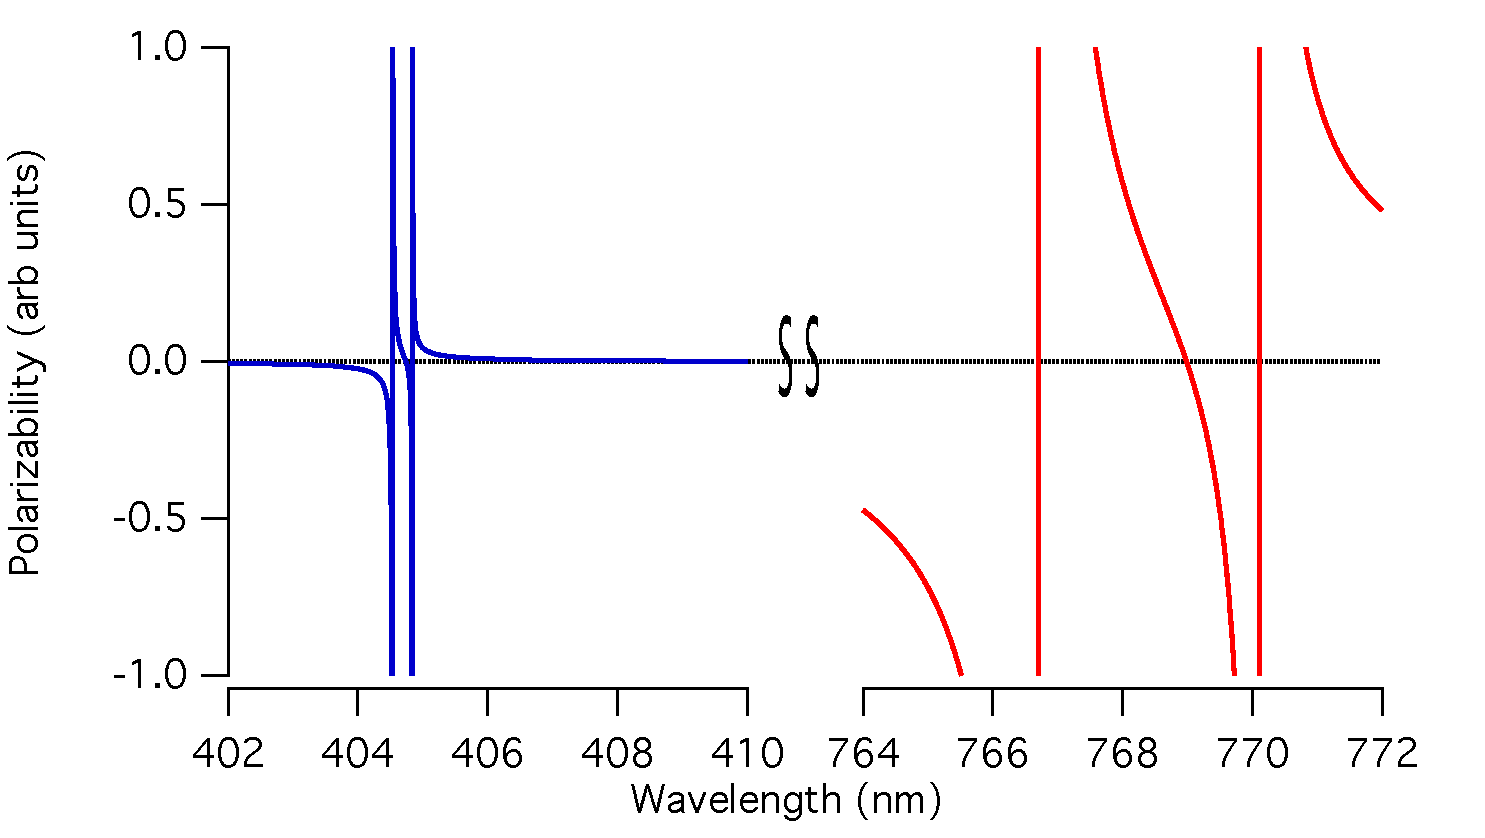
\includegraphics[width=1\textwidth]{Figures/KredBlueMZWedit.pdf}
\caption[Dynamic polarizability and magic-zero wavelengths of K.]{\label{KredBlueMZWfig}A plot of the dynamic polarizability of potassium in the vicinity of the $4s-4p$ (red) and $4s-5p$ (blue) transitions. Three zero-crossings, magic-zero wavelengths, are visible near 405 nm, 406 nm, and 769 nm. The blue and red transitions are shown using the same wavelength range to highlight the smaller fine structure splitting of the $4s-5p$ transitions.}
\end{figure}


Chapter \ref{mzwChapter} and Appendix \ref{mzwAppendix} describe in detail our measurement of the first magic-zero wavelength of potassium near 769.971 nm \cite{Hol12a}. This novel method to probe atom structure yielded the most precise determination of the ratio of the $D1$ to $D2$ line strengths. We found
\begin{eqnarray}
\label{Reqn}
R=\frac{S_2}{S_1}=\frac{|\langle 4s || D || 4p_{3/2}\rangle|^2}{|\langle 4s || D || 4p_{1/2}\rangle|^2}=2.0005(40).
\end{eqnarray}


Various $\lambda_\textrm{zero}$ have been used in experiments to study entropy exchange \cite{Cat09}, quantum information processing \cite{Dal08}, and diffraction of matter waves from an ultracold atom crystal \cite{Gad12}. We have also discussed future applications for magic-zero wavelengths such as measurements of hyperpolarizability, rotation sensing, additional line-strength measurements, and measurements of the contribution of core electrons to polarizabilities.


The longest magic-zero wavelengths for alkali atoms are determined mostly by the transition energies $\hbar\omega_1$ and $\hbar\omega_2$ and the ratio $R$ of the line strengths. We use the sum-over-states approach to describe the dynamic polarizability $\alpha(\omega)$ near these two transitions by
\begin{eqnarray}
\label{dynpol}
\alpha(\omega) = & \frac{1}{3\hbar} S_1 \left( \frac{\omega_1}{  \omega_{1}^2 - \omega^2} + R\frac{\omega_{2}} { \omega_{2}^2 - \omega^2} \right) + A
\end{eqnarray}
where $A$ accounts for contributions from core excitations, higher energy valence transitions, and core-valence coupling \cite{Saf06, Mit10}. At the longest magic-zero wavelength of potassium, $A$ is 0.02\% of the nearly equal and opposite contributions from the principal transitions to the polarizability and $A$ changes $\lambda_\textrm{zero}$ by 0.15(1) pm \cite{Saf12per}. Therefore, the theoretical uncertainty in this magic-zero wavelength calculation, 3 pm, is nearly entirely determined by uncertainty in the ratio of the line strengths, $R$. The total uncertainty of our $\lambdaZero$ measurement was 1.5 pm. 


To measure the magic-zero wavelength, we focused 500 mW of laser light asymmetrically on the paths of our interferometer. As stated previously, the energy shift of a polarizable atom is given by 
\begin{eqnarray}
U(\omega) = -\frac{1}{2} \alpha(\omega) \vec{E}^2(\omega,z,t)
\end{eqnarray}
where we now allow for a frequency dependence for the polarizability and the electric field. For optical frequencies, we can only measure the energy shift due to the time average of the electric field, i.e.~the intensity. The phase acquired along one interferometer path is given by $\alpha(\omega)$ and the intensity of the light $I(x,z)$ at that location:
\begin{eqnarray}
\label{mzwIntEqn}
\phi_0(\omega) = \frac{\alpha(\omega)}{2\epsilon_0 c \hbar v}\int_{-\infty}^{\infty}I(x,z) dz.
\end{eqnarray}
Similar to the static polarizability experiment, where we used a static electric field gradient, here, we use an intensity gradient to apply different phase shifts to each interferometer path. We measure the differential phase shift of the two interferometer paths. Measurements of these differential phase shifts as a function of optical frequency, or wavelength, allow us determine $\lambdaZero$.


The uncertainty of our $\lambdaZero$ measurement, 1.5 pm, was dominated by the reproducibility of the measurement. The statistical precision (2$\sigma$) of our experiment was 1.4 pm. Section \ref{mzwDataAnalysis} explains the relationship between the reproducibility and the data collection procedure in more detail. The broadband component of the light, shown in Figure \ref{ASEgratingPic}, was the largest source of systematic error (0.5 pm) in our measurement.


\begin{figure}
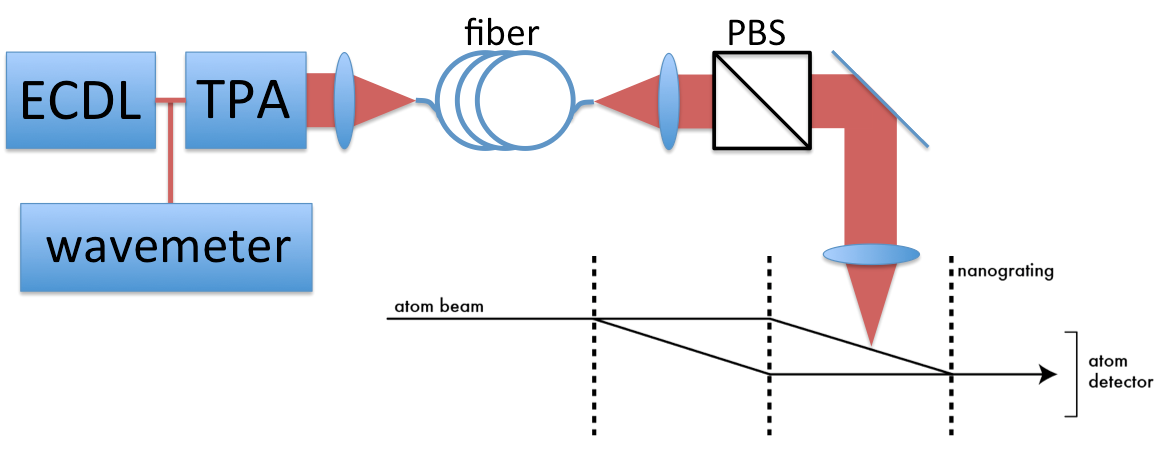
\includegraphics[width=1\textwidth]{Figures/mzwLaserSystem2.png}
\caption[Laser system for $\lambdaZero$ measurement.]{\label{mzwLaserSystem}Laser system for $\lambdaZero$ measurement. A grating-stabilized laser (ECDL) seeds a tapered amplifier (TPA). Light from the tapered amplifier is coupled into an optical fiber and then focused onto the atom interferometer. A wavelength meter measures the wavelength of the seed laser. Not shown is a shutter after the fiber to switch the light on and off, and an optical isolator on each side of the tapered amplifier.}
\end{figure}


%The laser spectrum is unfortunately not pure. Figure \ref{ASEgratingPic} shows the tapered amplifier light after being diffracted by a grating. Characterizing the laser spectrum is the leading contributor to the systematic uncertainty of our $\lambdaZero$ measurement.


\begin{figure}
\centerline{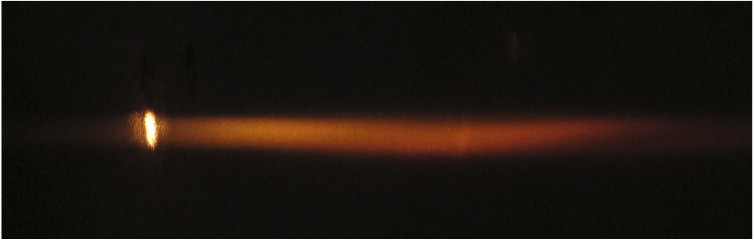
\includegraphics[width=.90\textwidth]{Figures/ASEpicture.png}}
\caption[Photograph of laser system spectrum.]{\label{ASEgratingPic}Photograph of the laser system spectrum. Light from the tapered amplifier was made to reflect off a diffraction grating and projected onto a screen. The spectrum shown spans approximately 50 nm. It is important to note that the photograph is a convolution of the frequency-dependent transfer function of the imaging system, including an infrared filter, with the spatially separated spectrum. Figure \ref{mzwSponData} shows the laser spectrum measured by a commercial grating spectrometer.}
\end{figure}


Interferometer contrast loss is primarily due to averaging over large distributions in phase shifts due to the atom beam velocity distribution and the nonuniform differential phase shifts across the atom beam. However, at the magic-zero wavelength we would naively expect zero phase shift for all atoms, and therefore no contrast loss. Unintended elliptical polarization of the laser beam combined with the unpolarized atom beam explains the contrast loss near $\lambdaZero$. Circular polarization causes different Zeeman substates ($m_F$) to acquire different phase shifts even at $\lambdaZero$. Section \ref{mzwContrast} explains the interferometer contrast loss in more detail.


This experiment can in principle be significantly improved before the photon scattering rate places a fundamental limit on the precision of a $\lambdaZero$ measurement. Let us imagine that we had unlimited laser power available and that we could focus all of the light on only one path of the atom interferometer to maximize the differential phase shift. Both the phase shift and the photon scattering rate grow in proportion to the laser power. However, the interferometer contrast, and thus the phase precision, decreases exponentially with the scattering rate. We therefore calculated a maximum achievable signal of 
\begin{eqnarray}
\label{TOWlimit}
\frac{d\phi}{d\omega}\approx\frac{1}{2\Gamma}P_\textrm{s}
\end{eqnarray}
where $P_\textrm{s}$ is the probability that an atom scatters one or more photons and $\Gamma$ is the excited state decay rate. With contrast loss due to scattering optimized to allow for maximum interferometric precision ($P_\textrm{s} = 1-e^{-1}$) the slope may become as large as $d \phi / d \lambda = $ 40 rad/pm. In this way, future measurements of magic-zero wavelengths can be made with very high precision, possibly with accuracy limited by a shot noise sensitivity better than picometers per $\sqrt{\textrm{Hz}}$. Section \ref{mzwLimitSection} contains a more detailed derivation of this limit.


Section \ref{mzwNextGenSec} discusses ideas to improve the precision of $\lambdaZero$ measurements in our lab. Improvements to the measurement precision would allow for benchmark tests of dipole matrix elements between the $ns$ and $(n+1)p$ levels in potassium and other alkali atoms. These matrix elements are more difficult to calculate due to larger relativistic corrections in the $(n+1)p$ levels. Interestingly, core electron contributions to polarizabilities may also be determined with $\lambdaZero$ measurements when combined with measurements of static polarizability and/or line strengths, depending on the particular atom and $\lambdaZero$. 







%%%%%%%%%%%%%%%%%%%%%%%%%%%%%%%%%%%%%%%%%
\pagebreak
\section{Strontium polarizability measurement proposal}
Polarizability measurements of strontium and ytterbium are currently highly desirable to support next-generation atomic clocks. The blackbody radiation environment surrounding atomic clocks changes the clock frequency by an amount proportional to the differential polarizability of the clock states and accurate polarizability measurements are required to calibrate this frequency shift. As an alkaline-earth atom with two valence electrons, strontium polarizability calculations are also more difficult due to electron correlations and call for experimental benchmarks. 


Unfortunately, our atom interferometer is currently unable to measure Sr polarizability due to low detection efficiency. Hot-wire detectors, like the one we use in our atom interferometer, do not ionize strontium atoms as efficiently as the alkali atoms. This is due to the ionization energy of strontium (5.7 eV) being larger than the work function of a platinum wire (5.5 eV). As a result, we presently can only detect collimated beams of strontium atoms in the absence of the nanogratings.


We propose that resonant photoionization can be used to provide high-efficiency and low-noise detection of strontium atoms. The photoionization pathway, shown in Figure \ref{srLevelsSimple}, involves absorption of a 461 nm photon to reach the $^1\textrm{P}_1$ state, and then absorption of a 405 nm photon to place the Sr atom in an autoionizing state. The existence of the autoionizing state increases the photoionization probability of Sr by a factor of about $10^3$.


\begin{figure}
\centerline{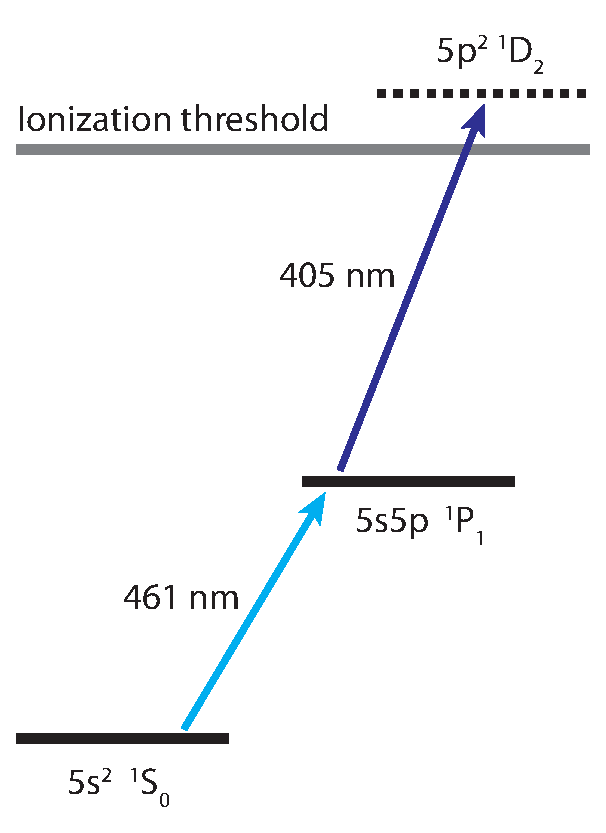
\includegraphics[width=.4\textwidth]{Figures/srLevelDiagramSimple.eps}}
\caption{\label{srLevelsSimple}Resonance enhanced photoionization pathway of strontium.}
\end{figure}


We propose a laser system consisting of a frequency doubled 922 nm laser diode and a free running 405 nm laser diode. A periodically poled KTP crystal can provide sufficient single pass frequency doubling efficiency (1-5\%), so we can avoid the complexity of a placing the crystal in a cavity. Generation of 1 mW of 461 nm light with less than 30 MHz linewidth and locked to the $^1\textrm{P}_1$ transition is the most difficult part of this proposed experiment. The 405 nm ionization laser can be relatively simple. The linewidth of the autoionizing transition is nearly 1 nm, so a high power 500 mW, multimode free running diode can be used.

Chapter \ref{alphaSrChapter} describes this proposal in more detail and is the topic of current research in our lab.






%%%%%%%%%%%%%%%%%%%%%%%%%%%%%%%%%%%%%%%%%
\pagebreak
\section{Tensor polarizability measurement proposal}

Ground-state alkali atoms are spherically symmetric, and as a result the polarizability may be described by a scalar that does not depend on the direction of the applied field. In contrast, molecules are generally not spherically symmetric and their polarizabilities must be described by a tensor $\tensorPol$. For a simple molecule such as an alkali dimer, the tensor is diagonal if one chooses to use the obvious axes of symmetry: one along the bonding axis of the molecule and two additional axes that are mutually orthogonal to the bonding axis. Figure \ref{dimerOrientationFig} shows the two unique orientations of an alkali dimer in an electric field. To our knowledge, only the average polarizability of this tensor has been measured \cite{Tar93,Mol74} for alkali dimers. Chapter \ref{dimersChapter} describes a proposal to measure the anisotropy of alkali dimer polarizability by studying contrast loss and revivals as a function of electric field strength. 

\begin{figure}
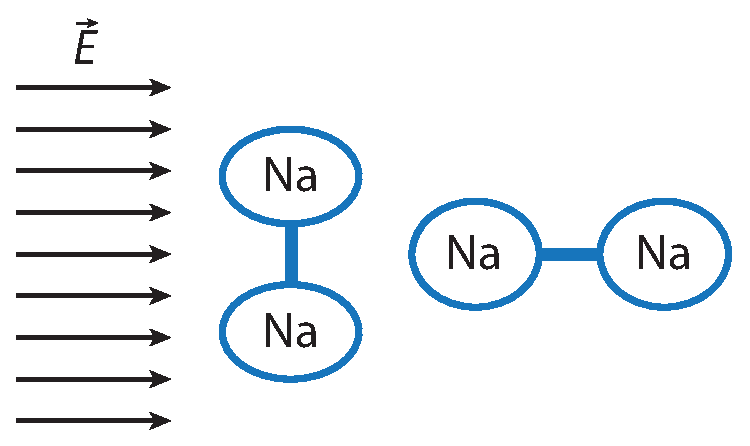
\includegraphics[width=1\textwidth]{Figures/dimerPolarizability.eps}
\caption[Alkali dimers in an electric field.]{\label{dimerOrientationFig}Two unique orientations of an alkali dimer with respect to the incident field. These two orientations have different polarizabilities, and thus different phase shifts in our atom interferometer.}
\end{figure}

%\begin{figure}
%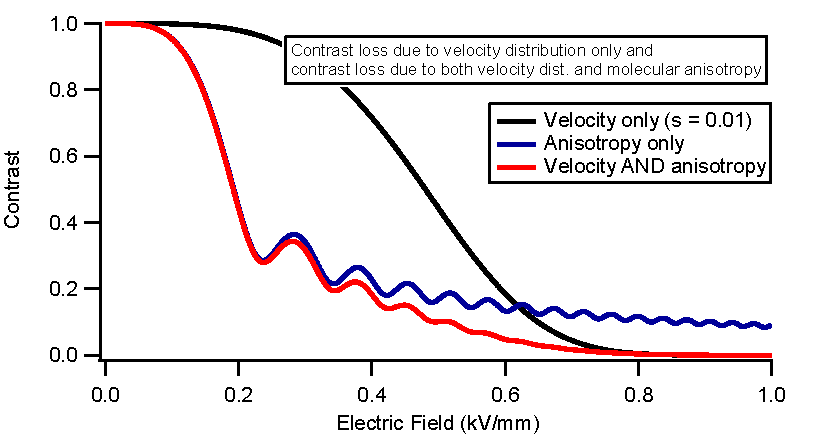
\includegraphics[width=1\textwidth]{Figures/molConVelAndGamma.pdf}
%\caption[Interferometer contrast loss due to the tensor polarizability of alkali dimers.]{\label{molConVelGammaBrief}Contrast loss due to anisotropy, velocity distribution, and both mechanisms combined. A measurement of the contrast loss signal may allow us to determine the polarizability anisotropy.}
%\end{figure}










\chapter{POLARIZABILITY MEASUREMENTS OF NA, K, AND RB}
\label{polChapter}

As introduced in Chapter 2, we measured the absolute and relative polarizabilities of sodium, potassium, and rubidium using a Mach-Zehnder atom interferometer with an electric-field gradient. Table \ref{polResultsTable} shows the absolute measurements (which have less than 1.0\% uncertainty), and Table \ref{polRatiosTable} shows the ratios of polarizability measurements (which we measured with 0.3\% precision). 


Our paper published in \emph{Physical Review A}, and shown in Appendix \ref{polPRAappendix}, explains the most important details of the experiment. In this chapter I provide supporting material. I explain how I improved the accuracy of the velocity measurements, I provide a reanalysis of the data set after discarding outliers, and I discuss subsequent improvements that I made to the polarizability measurement interaction region and data acquisition system.






%%%%%%%%%%%%%%%%%%%%%%%%%%%%%%%%%%%%
\section{Improved velocity measurement using a length gauge to study diffraction}
\label{polLG}
Section \ref{polBrief} described how the atom beam velocity was measured by studying diffraction data (see Figure \ref{nakrbDiffraction}). This technique determines the de Broglie wavelength of atoms in the beam, but it relies on accurate knowledge of the displacement of the hot-wire detector. The DC motors used to move components in our atom beam machine, including the detector translation stage, report their position using rotary encoders and knowledge of the screw pitch as a proxy for linear displacement. However, because of variations in the screw pitch and stick/slip behavior in the translation stage, these position reports are subject to as much as 15 $\mu$m errors in linear displacement of the translation stage. Since the diffraction orders are typically spaced by about 130 $\mu$m, this corresponds to a $\sim$10\% error in velocity. Figure \ref{intRegionMotorLG} shows the displacement reported by a typical motor vs the displacement reported by a length gauge.


To overcome this problem, I installed a Heidenhain MT-2571 length gauge to measure the detector displacement using a linear encoder. Figure \ref{velMotLG} shows atom beam velocities and velocity distribution widths determined by fitting diffraction data when using either the length gauge or the motor encoder to measure the detector position. The velocity measurement is clearly more reproducible when using the length gauge to measure detector displacement. I also note that it is possible that detector position measurement errors were significant and neglected in the Ekstrom \etal measurement of sodium polarizability \cite{Eks95}. The addition of this length gauge was also crucial for studies of van der Waals potentials using atom beam diffraction in our lab \cite{Lon09,Lon10}.


\begin{figure}
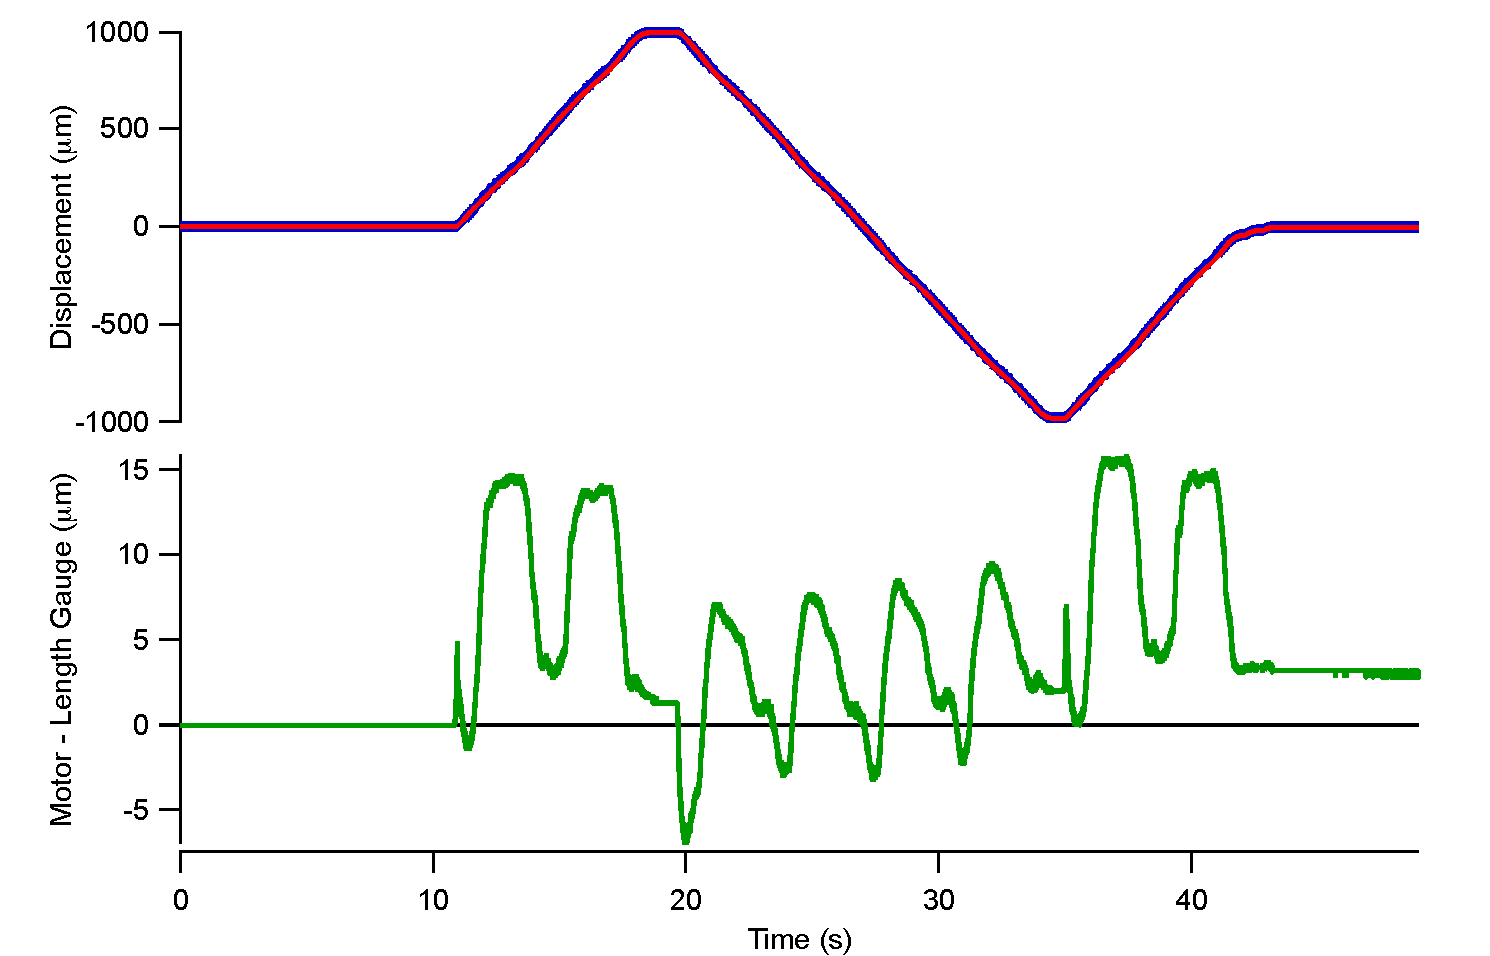
\includegraphics[width=1\textwidth]{Figures/motLGtrans.pdf}
\caption[Comparison of displacements measured by a motor encoder and a length gauge.]{\label{intRegionMotorLG}Displacement of the interaction region translation stage as measured by the motor encoder (blue) and a length gauge (red), and the difference in displacement measurements (green). Positive (negative) displacements correspond to retraction (extension) of the motor screw. Translating in the negative direction, corresponding to motor extension, is better for our experiments because the position error is lesser.}
\end{figure}



\begin{figure}
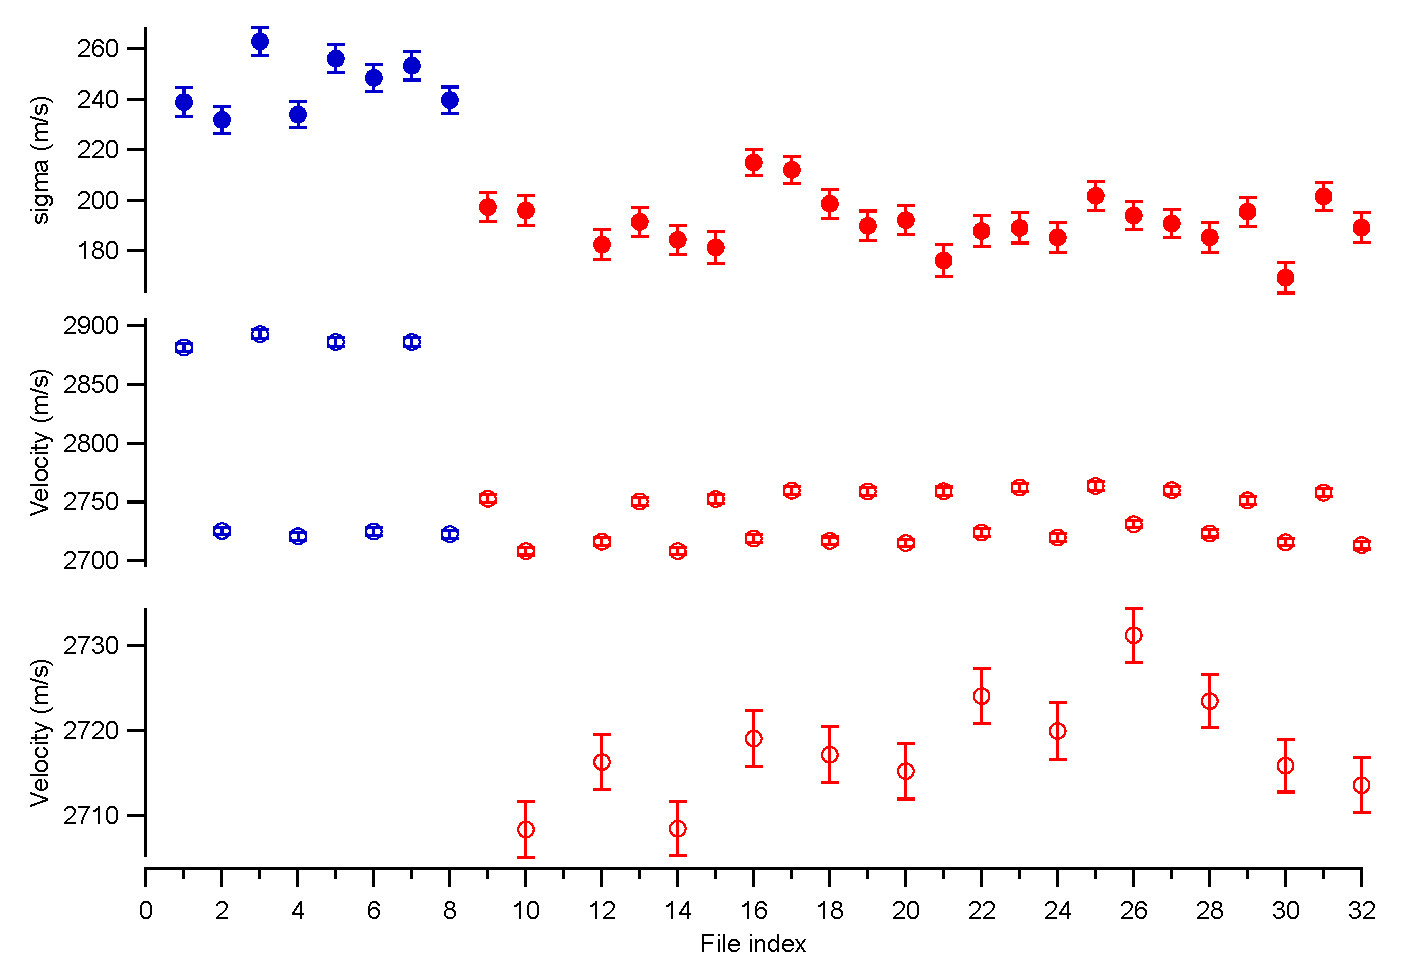
\includegraphics[width=1\textwidth]{Figures/velMotLG.pdf}
\caption[Atom beam velocities measured using a motor encoder and a length gauge.]{\label{velMotLG}Sodium atom beam velocity (open circles) and velocity distribution width (filled circles) using the detector motor (blue, files 1-8) or length gauge (red, files 9-32) to measure detector displacement. The up-down pattern in velocity reflects the fact that the motor direction was alternated and the translation stage exhibits stick/slip behavior. We only use the measurements corresponding to the extension of the motor screw (even numbered file indices), since this minimizes errors due to stick/slip of the translation stage. This subset of measurements yield $v=2717.8(6.5)$ m/s and $\sigma_v=190(11)$ m/s, where the uncertainties are the standard deviation and are statistical only.}
\end{figure}




%%%%%%%%%%%%%%%%%%%%%%%%%%%%%%%
\section{Reanalysis using a trimmed mean}
\label{trimMean2010}
I reanalyzed the 2010 polarizability data using a trimmed mean, so that the lowest and the highest 10\% of the data were discarded before calculating the mean and the standard error of the mean. This procedure is useful when outliers occur more frequently than a normal distribution of measurements would predict. Figure \ref{polPRAmeasurementsTrim}, Table \ref{polResultsTableTrim} and Table \ref{polRatiosTableTrim} show the results of this analysis. The statistical uncertainty of each polarizability measurement improves by about 20\%. As a result, the uncertainty of our measurements of $\alpha_\textrm{K}$ and $\alpha_\textrm{Rb}$ (determined by our ratio measurements of polarizabilities combined with the Ekstrom \etal measurement of $\alpha_\textrm{Na}$) improve slightly as well. These changes are well within the statistical uncertainty of the original measurements.


\begin{figure}
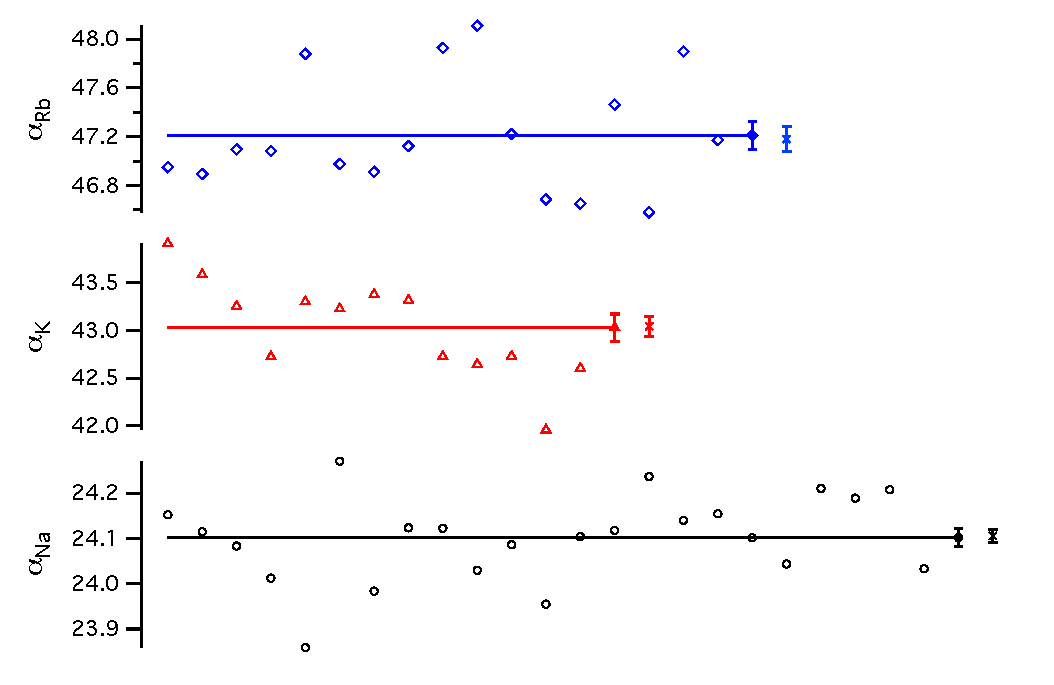
\includegraphics[width=1\textwidth]{Figures/polPRAdataTrim.pdf}
\caption[Multiple measurements of the polarizability of Na, K, and Rb and their trimmed means]{\label{polPRAmeasurementsTrim} Multiple measurements of the polarizability of sodium (circles), potassium (triangles), and rubidium (diamonds). The mean polarizabilities are denoted by filled markers and lines. The trimmed means are denoted by crosses. The error bars represent the standard error of the mean. Units are $10^{-24}$ cm$^3$. Final results are shown in Table \ref{polResultsTableTrim}.}
\end{figure}


\begin{table}
\caption[Measured absolute atomic polarizabilities using all data points and the central 80\%]{\label{polResultsTableTrim}Measured absolute atomic polarizabilities using all data points and the central 80\%. Also shown are the polarizabilities of K and Rb obtained using our ratios of polarizabilities using the central 80\% of the data (see Table \ref{polRatiosTableTrim}) combined with the sodium polarizability measurement from Ekstrom \etal \cite{Eks95}.}
\begin{center}
\begin{tabular}{c c | c | c}
\hline\hline
	& $\alpha_\textrm{abs All}$(stat.)(sys.) & $\alpha_\textrm{abs Trim}$(stat.)(sys.)  & $\alpha_{\textrm{Trim ratio \& Eks}}$(tot.)\\
\hline
Na & 24.11(2)(18) & 24.12(1)(18) & \\
K & 43.06(14)(33) & 43.08(11)(33) & 43.06(19)\\
Rb & 47.24(12)(42) & 47.21(10)(42)  &47.20(20)\\
\hline
\end{tabular}
\end{center}
\end{table}


\begin{table}
\caption{\label{polRatiosTableTrim}Measured atomic polarizability ratios with statistical uncertainties for the entire data set and the trimmed data set.}
\begin{center}
\begin{tabular}{c c c}
\hline\hline
 &  $\alpha_\textrm{ratio}$(stat.~unc.) \\
Atoms & All data & Trimmed \\
\hline
Rb/Na & 1.959(5) &1.958(4)  \\
K/Na    & 1.786(6) &1.786(5)  \\
Rb/K    & 1.097(5) &1.096(4)  \\
\hline\hline
\end{tabular}
\end{center}
\end{table}





%%%%%%%%%%%%%%%%%%%%%%%%%%%%%%%%%%%%
\section{Data acquisition system upgrades}
\label{newDAQ}

The 2010 polarizability measurements were accomplished by manually moving the interaction region and switching the high-voltage electrode on and off about once per minute. This quickly became mind-numbing, tedious work. Higher precision measurements of polarizability clearly demanded a more automated data acquisition system.

\begin{sidewaysfigure}
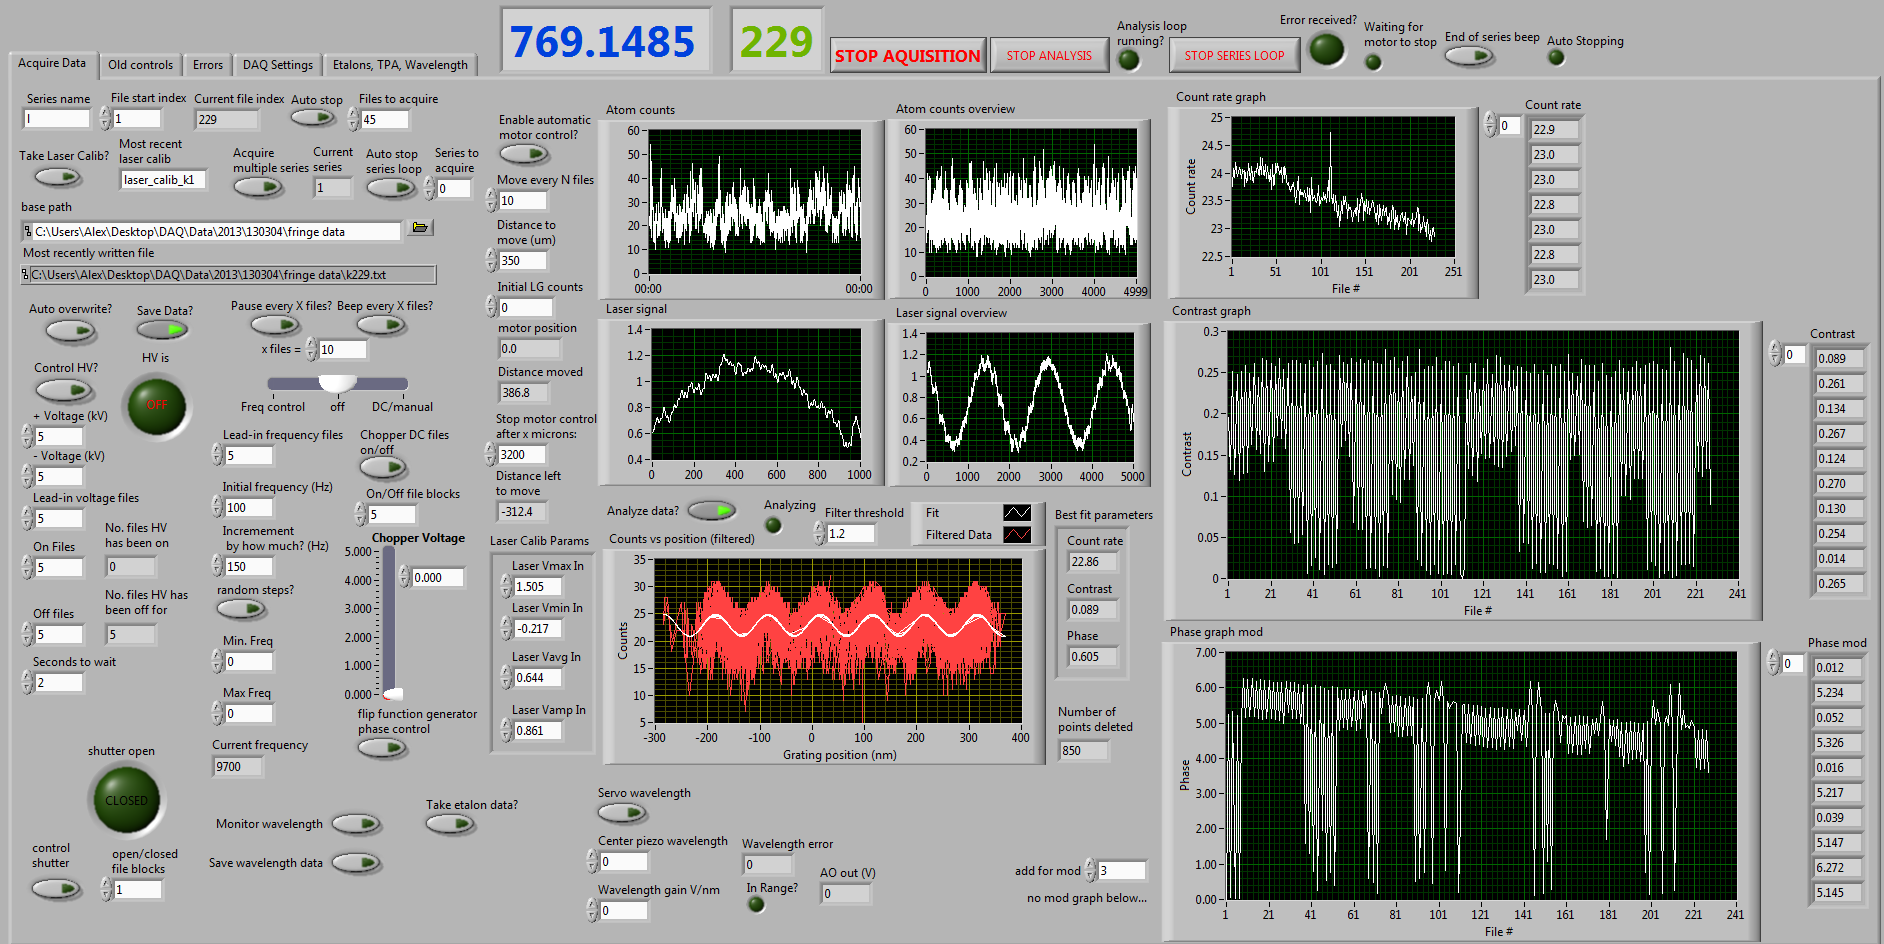
\includegraphics[width=1\textwidth]{Figures/daqScreenShotEdit.png}
\caption[Screenshot of the improved data acquisition system]{\label{DAQpicture}Screenshot of the data acquisition system. The left side contains experiment controls, such as data series name, the type of measurement (polarizability, velocity, or magic-zero wavelength), and high voltage settings. The middle section shows the atom count rate and laser interferometer data as a function of time and a plot of the interference fringe determined from the previous 5 s worth of data. Finally, the right side shows a history of the average count rate, contrast, and interferometer phase for the current data series. Additional tabs contain channel controls, error reporting displays, and some additional laser system monitors. While perhaps overwhelming at a glance, this suite of controls and instruments provides a significantly more powerful grasp of the experiment than the previous data acquisition system.}
\end{sidewaysfigure}


We developed a new data acquisition system in LabView 2010 with the ability to move and accurately record the distance traveled by any motor (via on-board quadrature decoding) in the atom beam machine and automatically control multiple high-voltage power supplies and a function generator. Figure \ref{DAQpicture} shows a screen shot of the data acquisition system. The new data-acquisition system uses a producer-consumer architecture to simultaneously record and analyze atom fringe data. This \emph{in situ} processing of atom fringe data has proven to be immensely valuable. Hardware controlled timing signals ensure that measurements of the atom beam count rate and the grating position are commensurate. A second screen enables viewing of the interferometer data from the optical table in our lab. 







%%%%%%%%%%%%%%%%%%%%%%%%%%%%%%%%%%%%
\section{Next-generation polarizability measurements}
\label{polChapterGradElg}

After publishing our 2010 polarizability measurements we designed a new experiment to improve both the precision and accuracy of polarizability measurements in our lab. We chose to replace the ground plane from the previous interaction region with a 2nd pillar. Figure \ref{IFMpillarsTrans} shows a schematic of the atom interferometer and a two-pillar interaction region. Figures \ref{newIntRegion2g} and \ref{intRegionNewPer} show a photo and a schematic of the new interaction region, respectively. The pillars are made of two 0.5 inch diameter rods separated by 3.81 mm. Figure \ref{twoPillarPolMeas} shows a measurement of cesium polarizability using the new interaction region.


As discussed in section \ref{polBrief}, the electric fields of the two regions are nominally identical, however, there are several advantages to the two-pillar geometry. First, two pillars allows us to measure phase shifts on both sides of the plane of symmetry in the electric field calculation. This in turn enables us to use phase shift data to independently determine both the polarizability and the position of the pillars relative to the atom beam. Measuring phase shifts on both sides of the symmetry plane also allows us to better control for the Sagnac phase shift. This is because the Sagnac phase shift makes the total phase shift closer to zero on one side of the pillars and farther from zero on the other, leading to an unambiguous signature. See Appendix A for a description of how the Sagnac phase shift effects the atom interferometer contrast and phase.


We also added a Heidenhain MT-2571 length gauge to measure the interaction region position. Irreproducibility in the interaction region position may have been a large source of the statistical error of the polarizability measurements in the first generation experiment. Section \ref{polLG} discussed the advantages of using a length gauge to measure displacement instead of relying on built-in rotary motor encoders.


Figure \ref{csPolNew} shows a single day of cesium polarizability measurements using the new electrodes, phase choppers for measuring atom beam velocity, and the new data acquisition system. Note the approximately 6 times improvement in statistical precision compared to our 2010 work, shown in Figure \ref{polPRAmeasurementsTrim}. Figure \ref{csPolVelDiff} shows consistent cesium polarizability measurements at three different atom beam velocities.



\begin{figure}
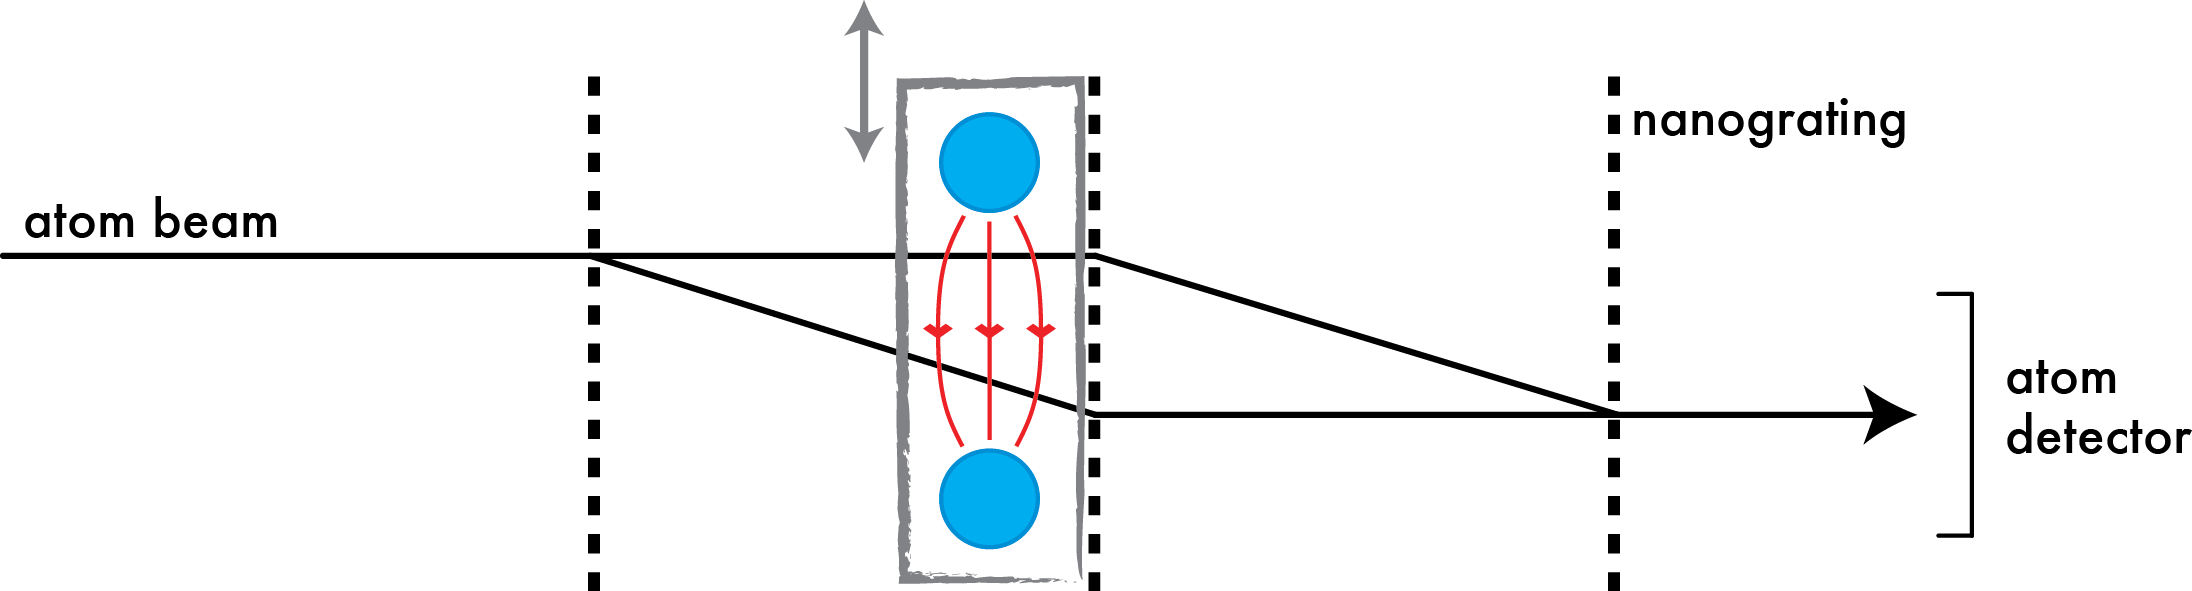
\includegraphics[width=1\textwidth]{Figures/IFMpillarsTrans.png}
\caption[Atom interferometer with two-pillar interaction region]{\label{IFMpillarsTrans}Atom interferometer with two-pillar interaction region. Measuring differential phase shifts as function of interaction region position, such as those shown in Figure \ref{twoPillarPolMeas}, allows us to determine the polarizability of an atom.}
\end{figure}


\begin{figure}
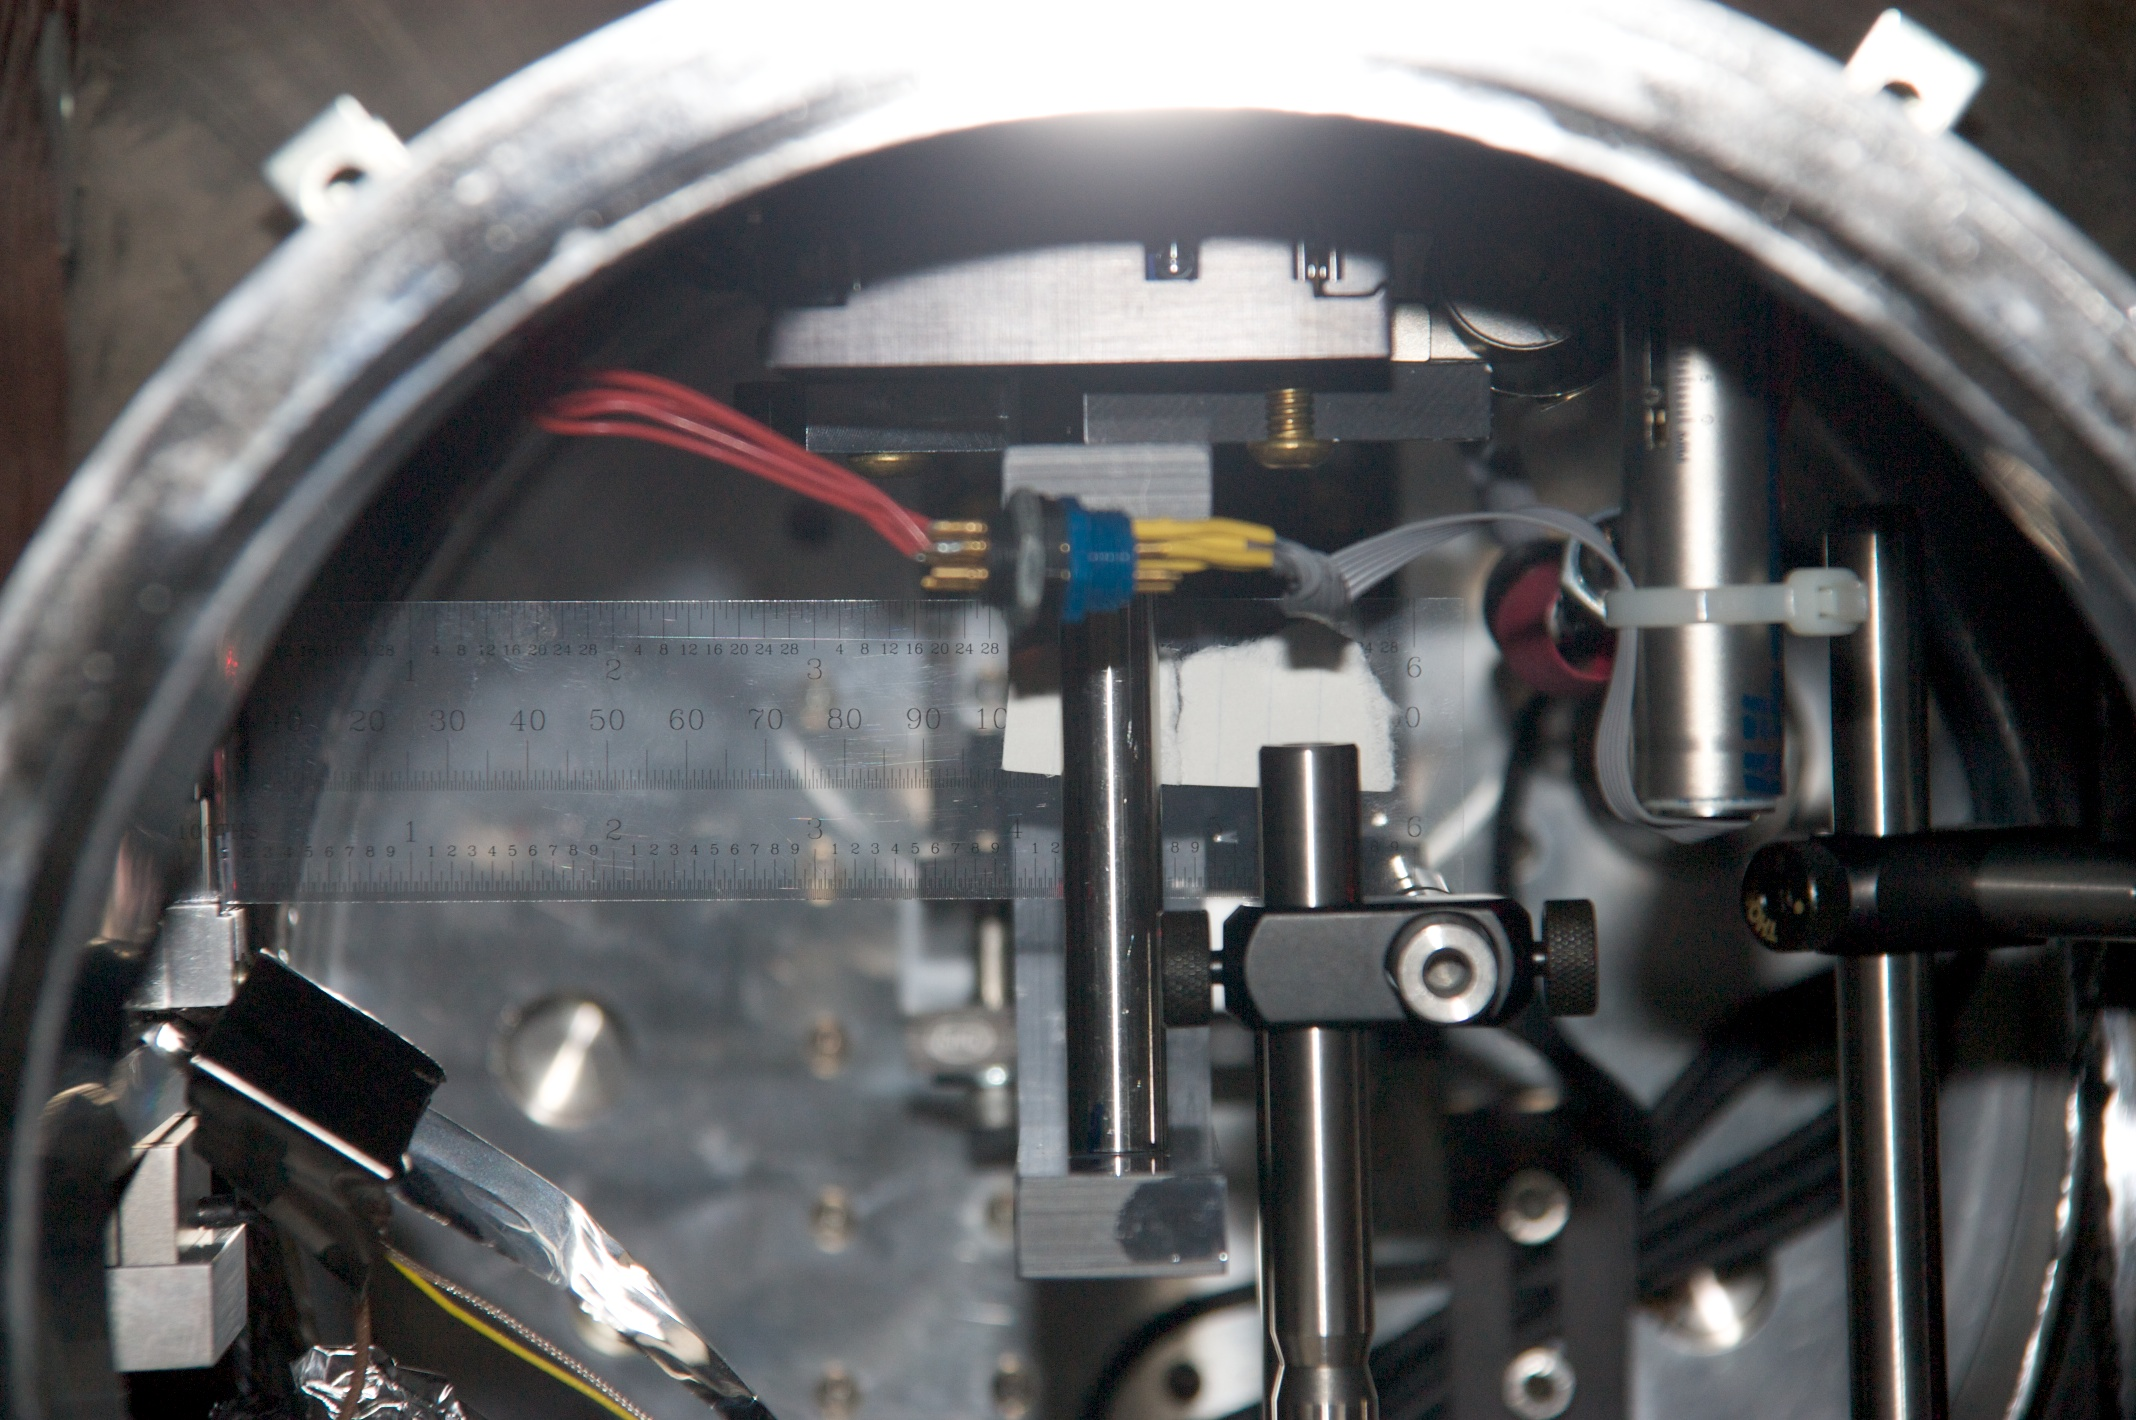
\includegraphics[width=1\textwidth]{Figures/intRegionNew2gMeas.jpg}
\caption[Measurement of the distance between the two-pillar interaction region and the 2nd nanograting]{\label{newIntRegion2g}Measurement of the distance between the two-pillar interaction region and the 2nd nanograting (left side, nearly edge-on).}
\end{figure}


\begin{figure}
\centerline{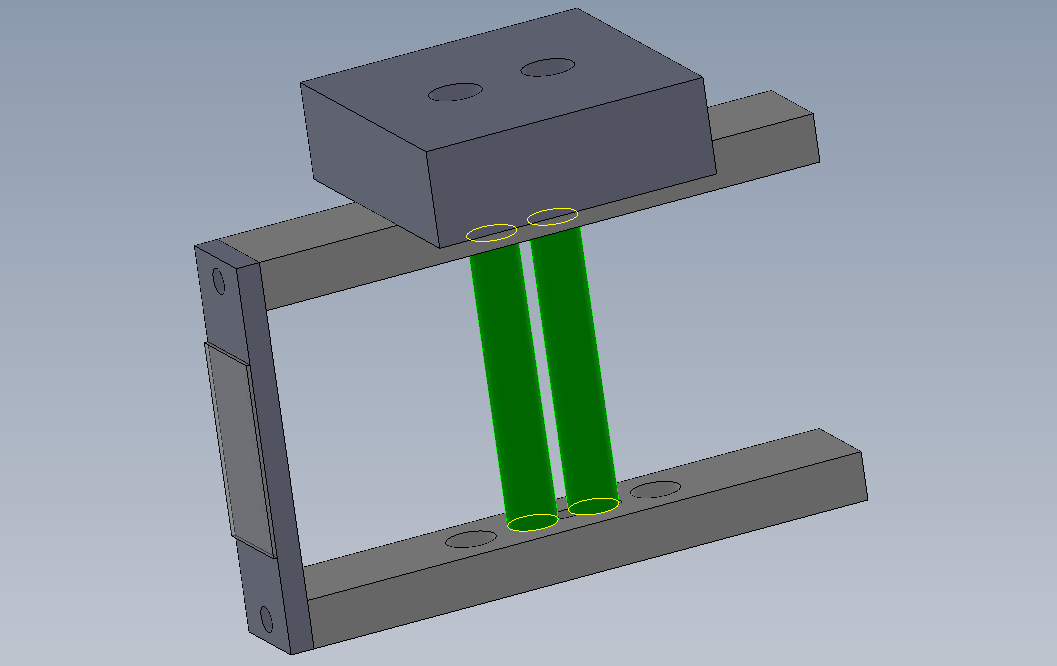
\includegraphics[width=0.75\textwidth]{Figures/intRegionNeweDrawings.png}}
\caption[Perspective rendering of the new interaction region]{\label{intRegionNewPer}Perspective rendering of the new interaction region. The electrodes (green) are held by PVC mounting bracket (light grey) and attached from below to a translation stage (dark grey). A microscope slide (semi-transparent) contacts a length gauge (not shown) for precise displacement measurements.}
\end{figure}


\begin{figure}
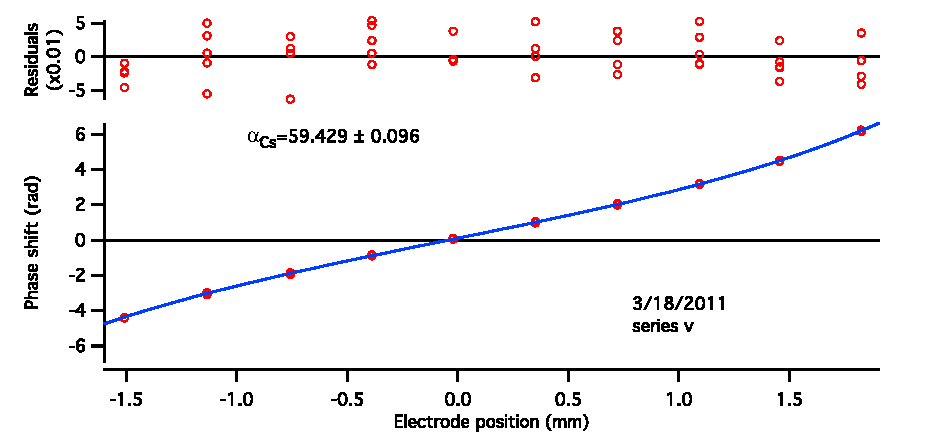
\includegraphics[width=1\textwidth]{Figures/twoPillarAlphaMeas.pdf}
\caption[Measurement of Cs polarizability using a two-pillar interaction region]{\label{twoPillarPolMeas}Measurement of cesium polarizability using a two-pillar interaction region. A least-squares fit to the phase shift data determines both the atomic polarizability and the atom beam position simultaneously. The reported uncertainty is statistical only.}
\end{figure}


\begin{figure}
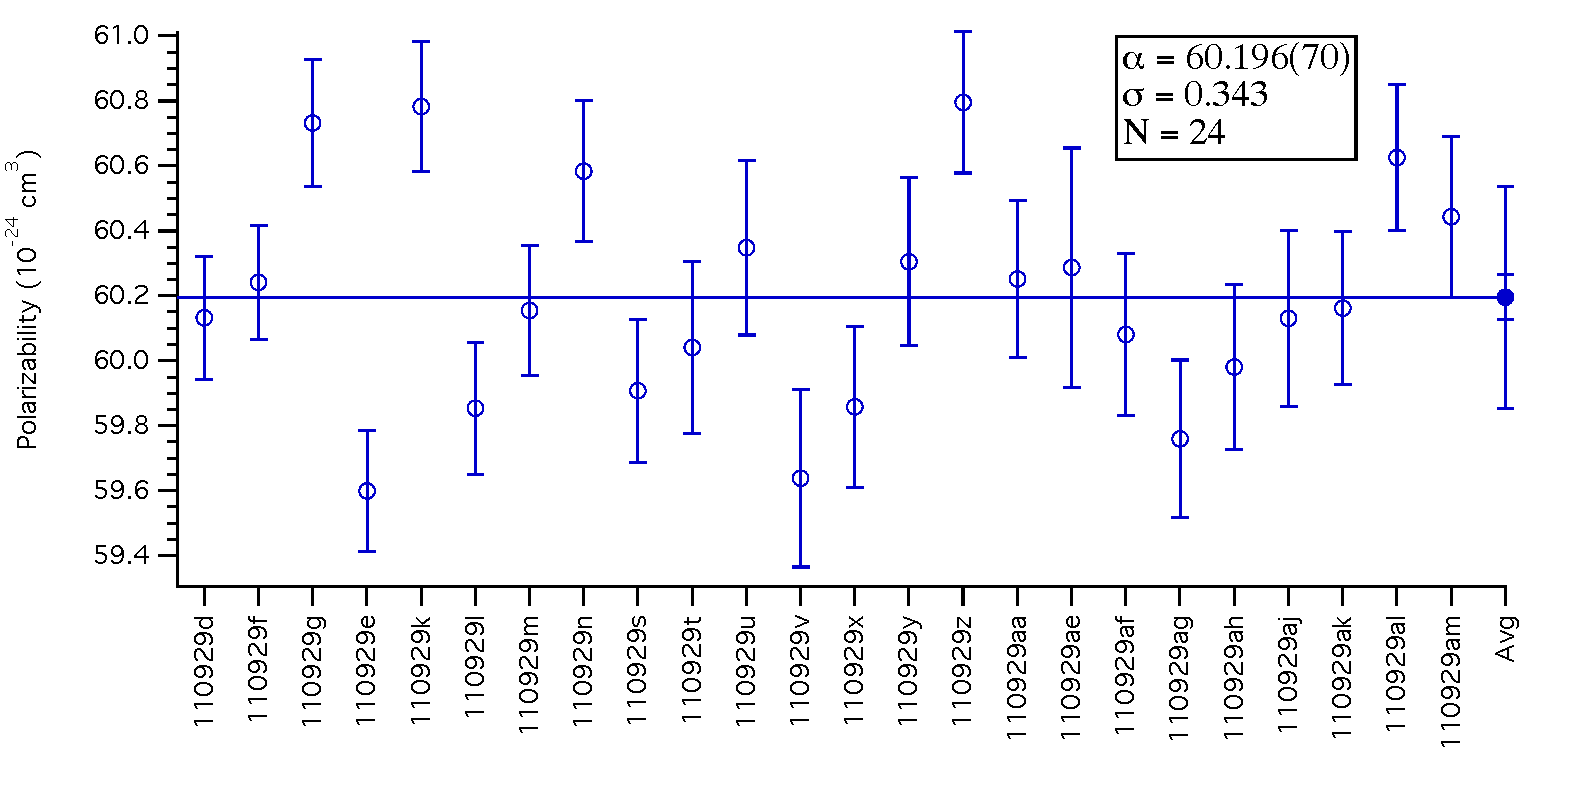
\includegraphics[width=1\textwidth]{Figures/csPol110929.pdf}
\caption[One day of polarizability measurements of Cs.]{\label{csPolNew}One day of polarizability measurements of cesium. The statistical precision (standard error of the mean) is 0.12\% (standard deviation of 0.5\%). However, the accuracy of this measurement is 1\% due to several uncalibrated parameters, such as the distance between the electrodes. The statistical uncertainty of each measurement is not used in determining the polarizability or the uncertainty, but is shown as a measure of consistency.}
\end{figure}


\begin{figure}
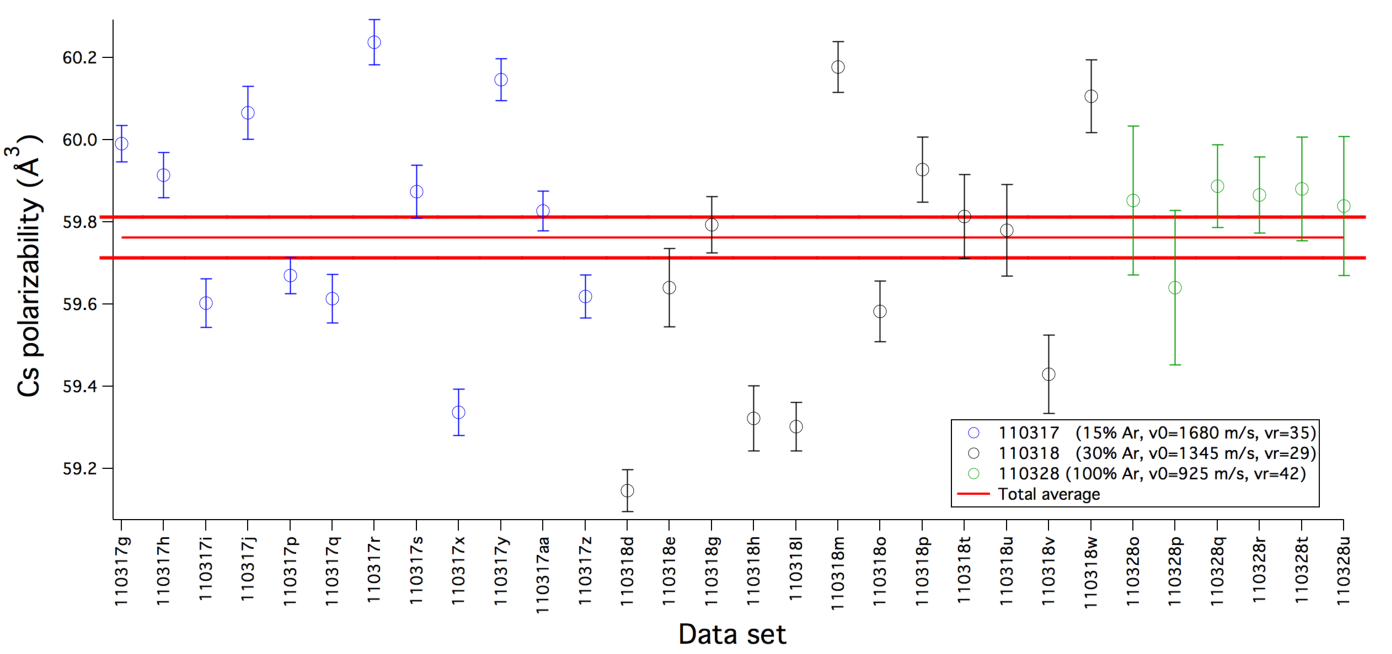
\includegraphics[width=1\textwidth]{Figures/csPolDifferentVels.pdf}
\caption[Consistent Cs polarizability measurements of at different velocities]{\label{csPolVelDiff}Consistent cesium polarizability measurements at three different velocities: 1680 m/s (blue), 1345 m/s (black), and 925 m/s (green). The total average and standard error of the mean is shown in red.}
\end{figure}



\chapter{MEASUREMENTS OF ATOM VELOCITY USING PHASE CHOPPERS}
\label{choppersChapter}

Section \ref{choppersBrief}, Appendix B and C.E. Klauss' B.S.~thesis \cite{Kla11} discuss our use of phase choppers to measure atom beam velocity. Section \ref{polChapterGradElg} shows polarizability measurements obtained after measuring atom beam velocity using phase choppers. Here, we provide samples of the pictures used to determine the distance between the phase choppers. I also discuss the ability of phase choppers to act as lenses for atomic de Broglie waves.




%%%%%%%%%%%%%%%%%%%%%%%%%%%%%%%%%%%%%%%%%%%%%%
\section{Distance measurements using high resolution pictures}
\label{distMeasurements}
The accuracy of the velocity measurement using phase choppers can only be as good as the measurement of the distance between the two choppers. To measure this distance (and others in the machine) we carefully inserted a series of rulers and tape measures into the vacuum chamber and took high resolution pictures of the choppers next to the measuring devices, such as the ones shown in Figure \ref{distMeas_c1e_c2w} and Figure \ref{distMeas_2g}. We mounted the camera (a Canon PowerShot S90) on a translation stage to accurately center the high-voltage wire in the middle of the frame and avoid angular misalignments. This minimized errors due to distortion and parallax. We then used optical and digital zoom to determine the positions of the choppers with respect to the tape measures with 100 $\mu$m precision. We used additional rulers and calipers to calibrate the accuracy of the tape measure.


We also took additional pictures with a vertically oriented ruler to determine the height at which the atom beam crosses the phase choppers, as well the angle of the choppers with respect to vertical by placing a plumb line next to the choppers. An example of the plumb line is shown in Figure \ref{distMeas_c1e_c2w}. These two measurements are combined to measure the distance between the two choppers where it counts: at the height of the atom beam. 


\begin{figure}
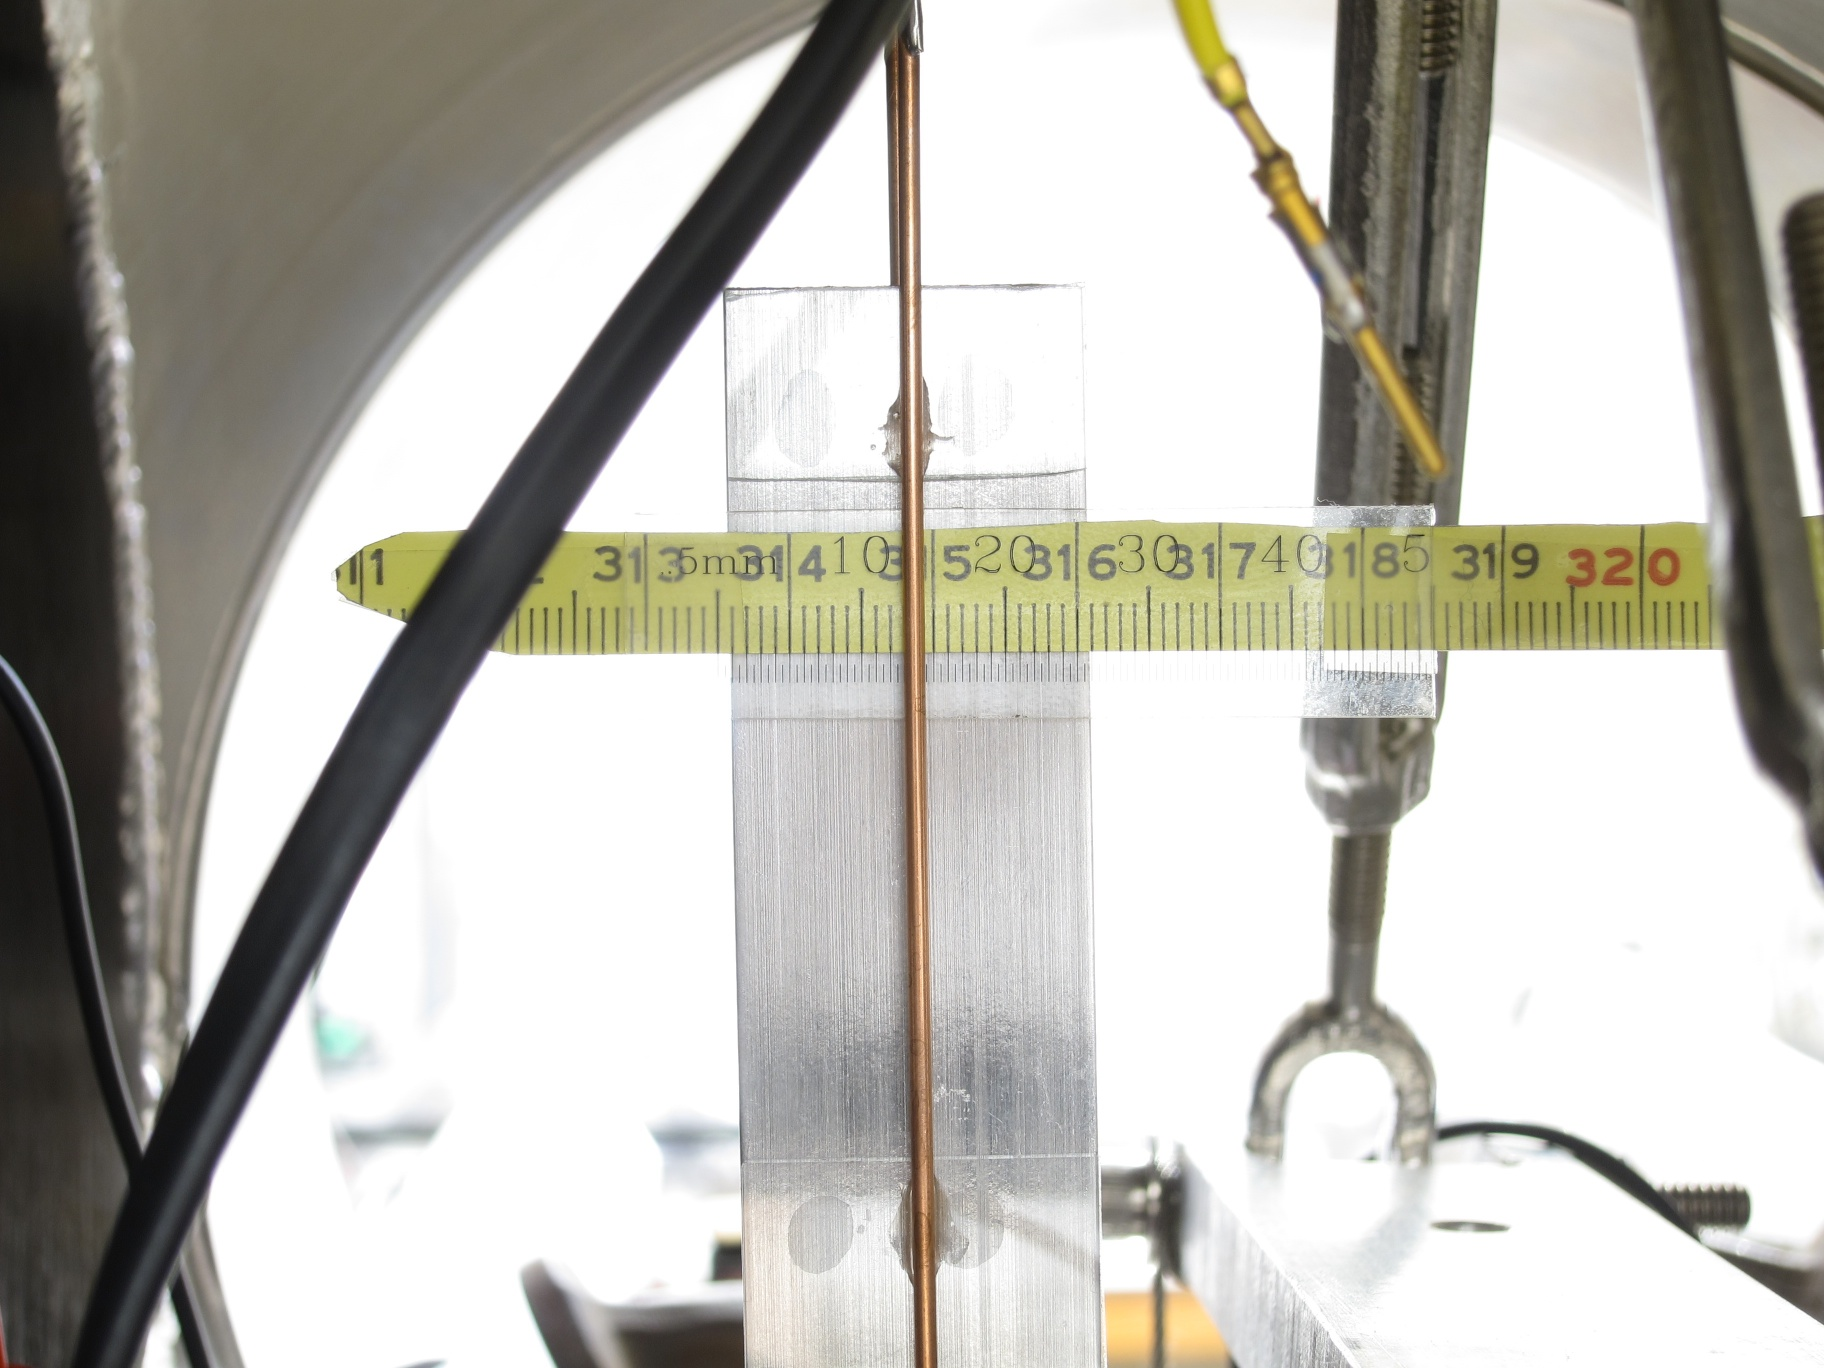
\includegraphics[width=0.5\textwidth]{Figures/distMeas_c1e.jpg}
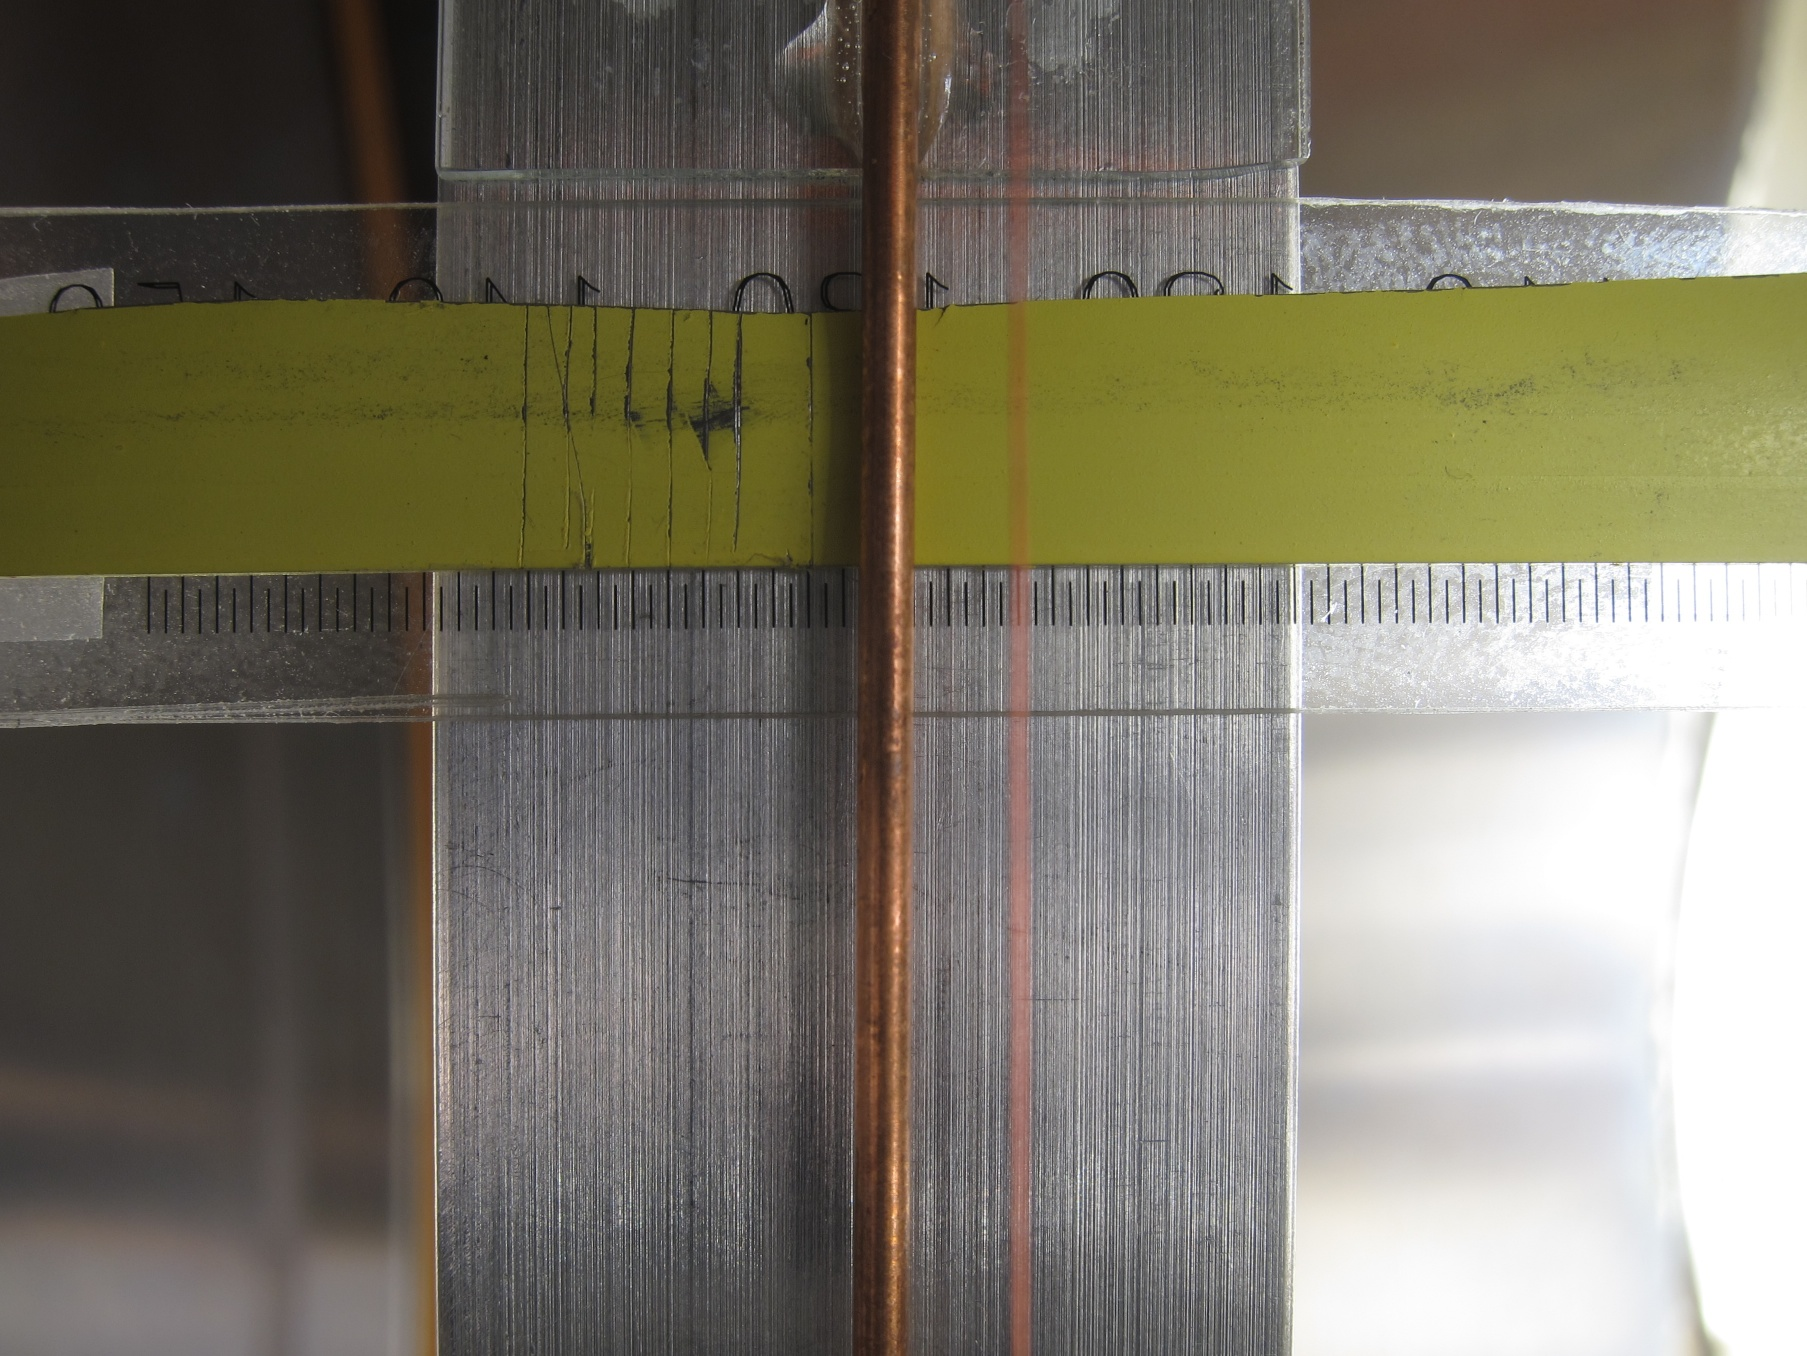
\includegraphics[width=0.5\textwidth]{Figures/distMeas_c2w.jpg}
\caption[Photographs for the measurement of the distance between chopper 1 and chopper 2.]{\label{distMeas_c1e_c2w}Measurement of the distance between chopper 1 and chopper 2 using a tape measure strung through the vacuum chamber above the atom beam path. Chopper 1 east side (left), and chopper 2 west side (right) are pictured. A transparent ruler serves as a translator between the two sides of the tape measure. The total uncertainty of this distance measurement is 250 $\mu$m. A plumb line (red) next to chopper 2 is also shown. Figure \ref{distMeas_2g} shows the approximate midpoint of the ruler above the 2nd nanograting.}
\end{figure}


\begin{figure}
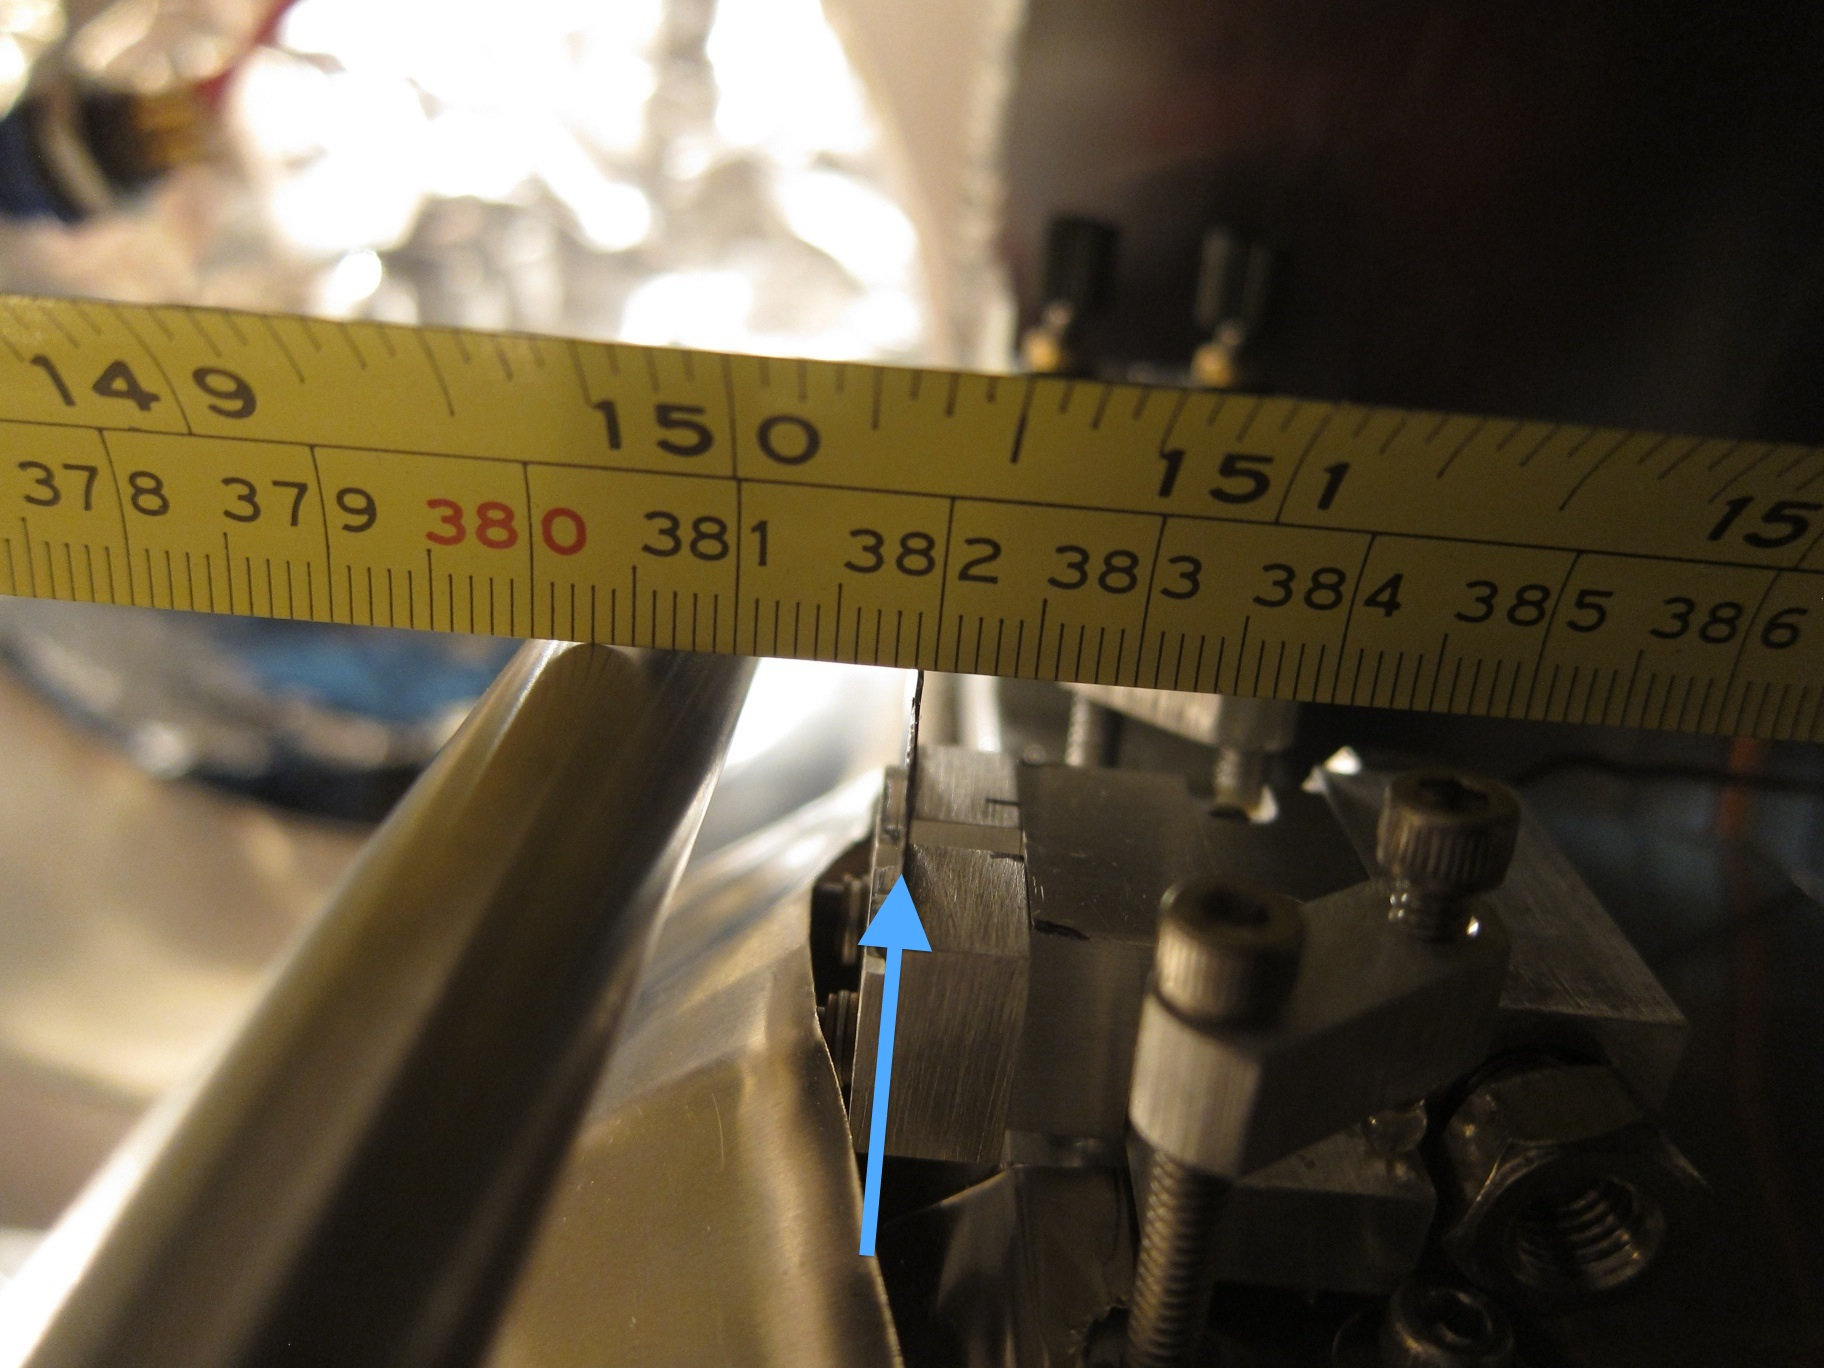
\includegraphics[width=1\textwidth]{Figures/distMeas_2g_arrow.jpg}
\caption[Photograph for the measurement of the distance between chopper 1 and chopper 2 showing the 2nd nanograting.]{\label{distMeas_2g}Measurement of the distance between chopper 1 and chopper 2. Two different nanogratings (both suitable for use as the second nanograting in the interferometer) are viewed edge-on and highlighted with a blue arrow. This allows us to determine the position of the 2nd grating with respect to the two phase choppers.}
\end{figure}





%%%%%%%%%%%%%%%%%%%%%%%%%%%%%%%%%%%%%%%%%%%%%%
\section{An electrostatic lens for matter waves inside an atom interferometer}
\label{lensSection}
In trying to reconcile small but persistent differences between the expected and observed interferometer contrast when using phase choppers, we discovered that our phase choppers can act as a lens for matter waves in our atom interferometer. Phase choppers, like all of the interaction regions described in this thesis, apply phase shifts that are a function of atom beam velocity. We would therefore naively assume that this dispersive phase shift would lead to a decrease in the measured contrast due to the velocity distribution of the atom beam. Instead, we observed that chopper 2 could \emph{increase} the interferometer contrast. Figure \ref{c2dcIncrease} shows an example of the interferometer contrast increasing when chopper 2 applies a differential phase shift. 


The key to understanding this effect is to realize that we detect the fringes formed by two complementary interferometers (formed by the +1, 0, and -1 diffraction orders from the first nanograting) and that the fringes formed by the two interferometers will not have the same phase unless the distance between the first and second nanogratings is exactly equal to the distance between the second and third nanograting. That is, if $d_\textrm{1G2G} \neq d_\textrm{2G3G}$ there will be a phase mismatch between the two interferometers, and thus a loss of contrast. Figure \ref{lens2IFM} shows a two interferometer model with chopper 1, the polarizability pillars, and chopper 2. Any of these electrodes can in principle correct for a phase mismatch between the two interferometers, provided that the sign of the phase shift is correct and the contrast loss due to the velocity distribution is negligible. However, chopper 2 can more easily correct the phase mismatch because of the larger spatial separation between the two interferometers at its location. This process is analogous to a diverging lens for matter waves in the atom interferometer acting to magnify the atom interference fringes. The consequences of this mechanism will be detailed in a future publication from our group.


Our \emph{New Journal of Physics} paper \cite{Hol11}, included in Appendix B, acknowledges that we could not explain the small difference between the measured reference contrast and the best-fit contrast determined using $\chi^2$ minimization. This problem was largely irrelevant to the determination of the atom beam velocity because it does not directly effect the frequencies at which the contrast revivals and minima occur. The contrast discrepancies do, however, effect the determination of the width of the velocity distribution. This in turn slightly changes the best estimate of the average velocity. In Holmgren \etal \cite{Hol11}, we estimated a 0.04\% systematic error in velocity may be present due to this discrepancy. We now understand that the magnitude of the error depends on the distance mismatch between the three nanogratings and may be several times larger unless we take more care to align the interferometer. Clearly, the highest accuracy measurements of atom beam velocity demand a full understanding of the data, and we are developing a more sophisticated model to incorporate these lensing effects.


\begin{figure}
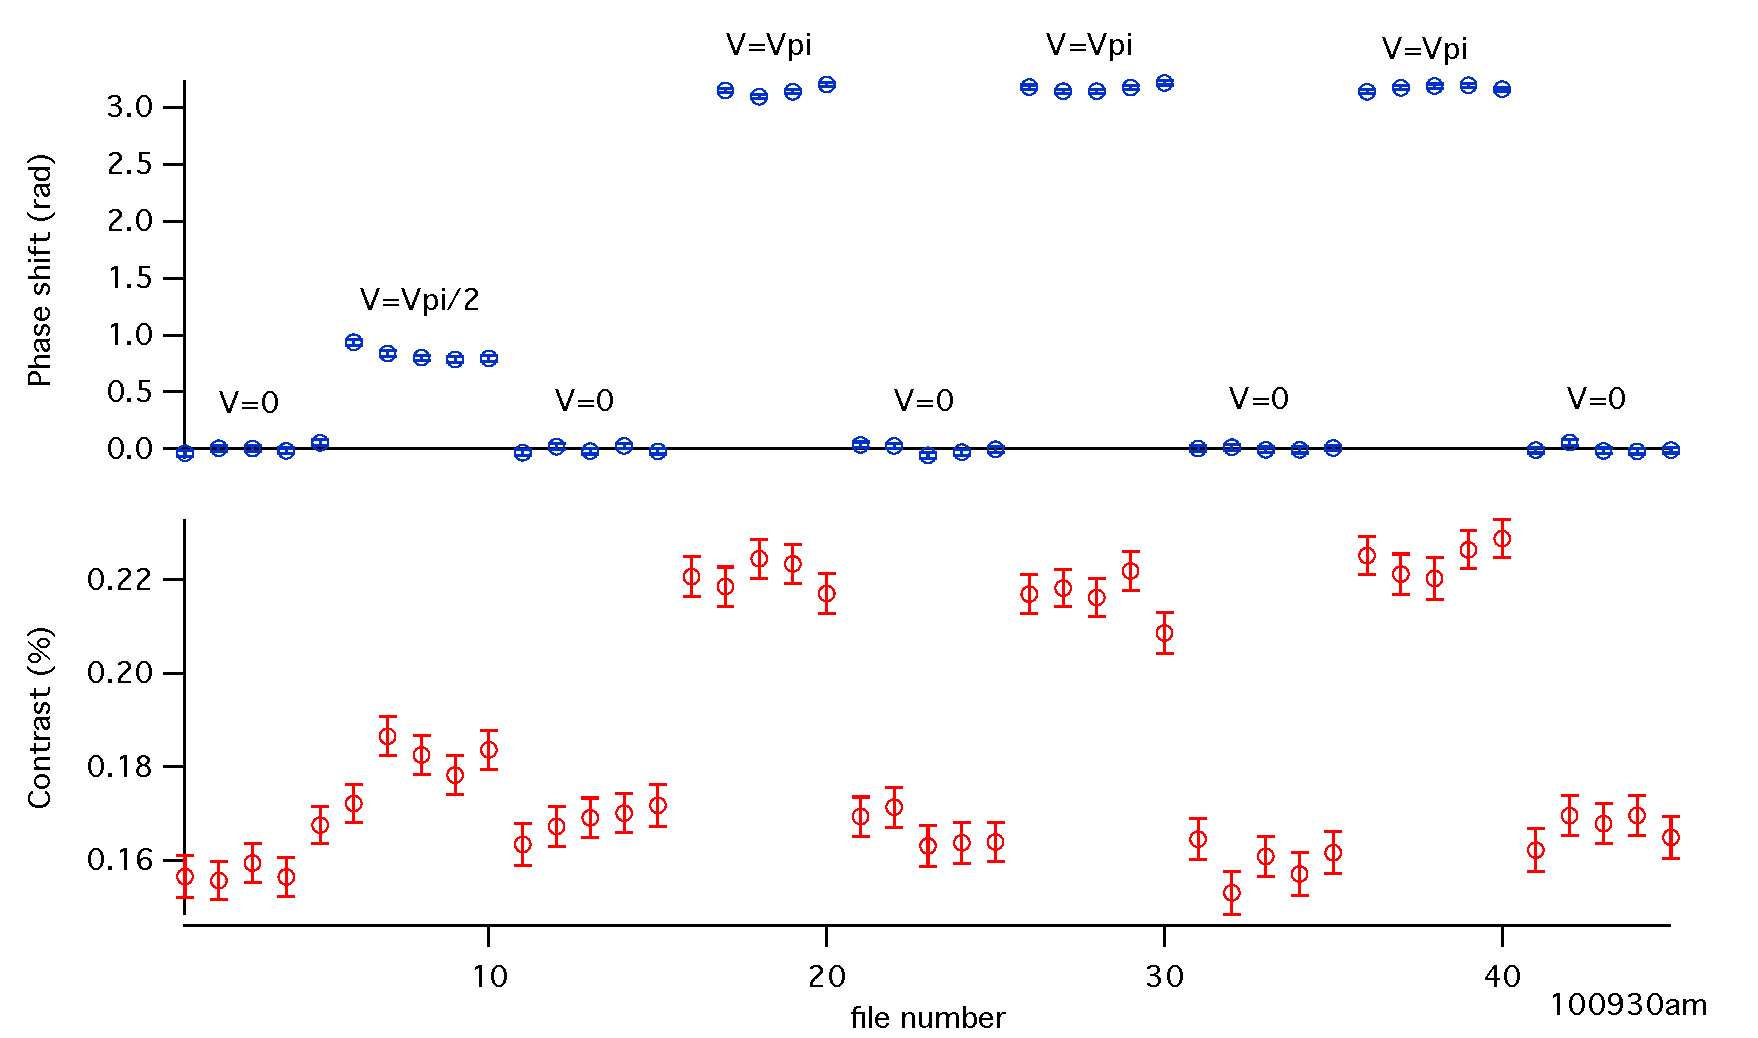
\includegraphics[width=1\textwidth]{Figures/contrastIncrease.pdf}
\caption[Unexpected increase in interferometer contrast due to energizing phase chopper 2.]{\label{c2dcIncrease}Interferometer phase shift (blue) and contrast (red) for three different voltages applied to chopper 2. $V_\pi$ is the voltage necessary to create a $\pi$ phase shift. The interferometer contrast \emph{increases} when a voltage is applied due to the \emph{rephasing}, or alternatively, the \emph{lensing} ability of chopper 2.}
\end{figure}


\begin{figure}
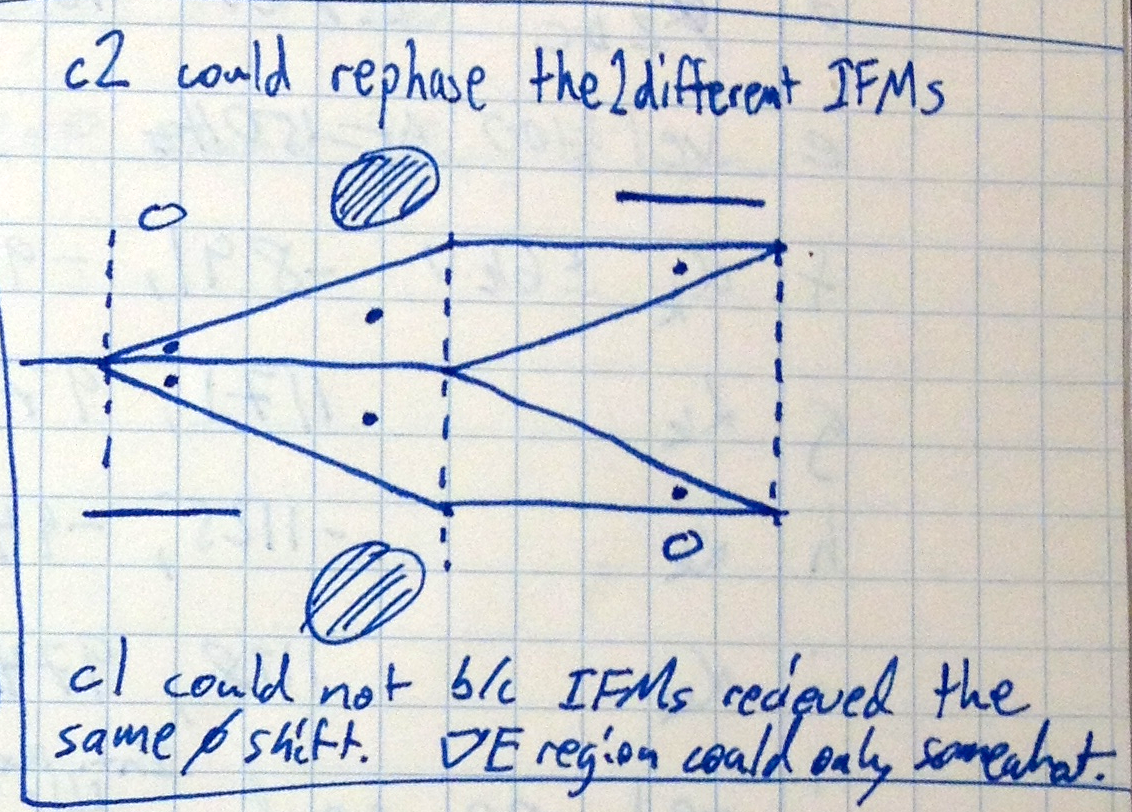
\includegraphics[width=1\textwidth]{Figures/lens2IFMnotebook.png}
\caption[Sketch of chopper 1, the polarizability electrodes, and chopper 2 with a two interferometer model.]{\label{lens2IFM}Nanogratings form multiple interferometers whose centerlines (marked with dots) diverge as a function of distance from the first nanograting. These two interferometers acquire different phase shifts because the electric field gradient is not uniform. The mismatch between interferometer phase shifts normally leads to a loss of observed contrast, but it can also lead to an increase in observed contrast if the distance between the first and second nanogratings is not equal to the distance between the second and third nanogratings. The phase choppers c1 and c2 are represented by small circles and thin lines (see Figure \ref{choppersIFMsimple}) and the polarizability interaction region is represented by slashed circles (see Figure \ref{IFMpillarsTrans}). Figure from page 31 of Tucson Book 13, October 5, 2011.}
\end{figure}





\chapter{MEASUREMENT OF A MAGIC-ZERO WAVELENGTH}
\label{mzwChapter}

Section \ref{mzwBrief} and Appendix \ref{mzwAppendix} describe our measurement of the first $\lambdaZero$ of potassium, published in \emph{Physical Review Letters} (2012) \cite{Hol12a}. In this chapter I will discuss the relationship between dynamic polarizability, oscillator strengths, and line strengths. I will then discuss our data analysis procedures, derive the fundamental limit to the precision of any $\lambdaZero$ measurement, discuss contrast loss mechanisms, and discuss the effect of an impure optical spectrum on $\lambdaZero$ measurements. Finally, I will discuss several possible new experiments to improve the precision of $\lambdaZero$ measurements. 


\section{Polarizability, oscillator strengths, matrix elements, and all that}
\label{dynPolSec}
The dynamic polarizability $\alpha(\omega)$ can be written most compactly in atomic units as
\begin{eqnarray}
\label{alphaOmegaFeqn}
\alpha(\omega)=\sum_k\frac{f_{k}}{\omega_k^2-\omega^2}
\end{eqnarray}
where $f_k$ is the oscillator strength. Note that the conversion between frequency in atomic and S.I. units is
\begin{eqnarray}
\label{omegaAUSI}
\omega_\textrm{a.u.}&=&\frac{\hbar}{E_h}\omega_\textrm{SI}\nonumber\\
&\approx&\frac{\omega_\textrm{SI}}{4.1341\times10^{16} \textrm{ Hz}} .
\end{eqnarray}
The sum of $f_k$ is approximately equal to the number of valence electrons, i.e.~1 for alkali atoms and 2 for alkaline-earth atoms. $f_k$ is related to the reduced dipole matrix elements through
\begin{eqnarray}
\label{fEqn}
f_k=\frac{2 |\langle \psi || D || \psi_k \rangle|^2 \omega_k}{3(2j+1)}
\end{eqnarray}
where $j$ is the degeneracy of the state of interest, $|\psi\rangle$, and $D$ is the dipole operator. For ground state alkali atoms, $J=1/2$, so $j=2$. We can combine equations \ref{alphaOmegaFeqn} and \ref{fEqn} to write the dynamic polarizability as
\begin{eqnarray}
\label{alphaOmegaMatrixElmEqn}
\alpha(\omega)=\frac{2}{3(2j+1)}\sum_k \frac{|\langle \psi || D || \psi_k \rangle|^2 \omega_k}{\omega_k^2-\omega^2}.
\end{eqnarray}
It is also common to refer to a line strength $S_k = |\langle \psi || D || \psi_k \rangle|^2$. Using this definition, the polarizability becomes
\begin{eqnarray}
\label{alphaOmegaSeqn}
\alpha(\omega)=\frac{2}{3(2j+1)}\sum_k \frac{S_k \omega_k}{\omega_k^2-\omega^2}.
\end{eqnarray}
I have found the conversion of quantities between atomic and S.I. units to be easy to miscalculate and I recommend checking every calculation against a benchmark such as static polarizabilities, transition energies, and literature values of matrix elements. In addition, I recommend keeping a copy of Hilborn's article ``Einstein coefficients, cross sections, f values, dipole moments, and all that" \cite{Hil82} nearby.


So far we have only considered the valence electrons in our polarizability model. Equation \ref{alphaOmegaFeqn} is typically modified to include a core polarizability term, $\alpha_\textrm{core}$, and a valence-core coupling term, $\alpha_\textrm{vc}$:
\begin{eqnarray}
\label{alphaOmegaCore}
\alpha(\omega)=\sum_k\frac{f_{k}}{\omega_k^2-\omega^2} + \alpha_\textrm{core} + \alpha_\textrm{vc}.
\end{eqnarray}
The core and valence-core coupling terms do not have a significant frequency dependence in the optical range. In addition, the valence term is typically broken up into the strongest terms that are explicitly written out with a frequency dependence, plus a ``tail" contribution that is frequency independent and small. When considering the polarizability in the vicinity of the D1 or D2 lines in alkali atoms it is often sufficient to write
\begin{eqnarray}
\label{alphaOmegaTail}
\alpha(\omega)=\frac{f_{D1}}{\omega_{D1}^2-\omega^2} + \frac{f_{D2}}{\omega_{D2}^2-\omega^2} + \alpha_\textrm{tail} + \alpha_\textrm{core} + \alpha_\textrm{vc}.
\end{eqnarray}
The rotating wave approximation, $\omega_{0}^2-\omega^2 \approx 2\omega_0(\omega_0-\omega) = 2\omega_0\Delta$, can also be used to simplify the polarizability near resonance. A factor of $\omega_0$ conveniently cancels in the numerator and the denominator when expressing polarizability near resonance using the line strengths $S_k$:
\begin{eqnarray}
\label{alphaOmegaRWA}
\alpha(\omega)=\frac{2}{3(2j+1)}\sum_k   \frac{S_k}{\Delta_k}.
\end{eqnarray}
Static terms corresponding to tail, core, and valence-core contributions can be added if desired.


Table \ref{kMZWcontTable} summarizes the contributions of each of these parameters near the first magic-zero wavelength of potassium. Uncertainties in the $4s$ to $4p_{1/2}$ (D1) and $4p_{3/2}$ (D2) line strengths dominate the uncertainty of $\lambdaZero$. Our $\lambdaZero$ measurement determines the ratio of these line strengths. Future measurements of additional $\lambdaZero$ in potassium and other atoms will determine different ratios of matrix elements or the core polarizability, depending on the the relative uncertainties of these parameters.



\begin{table}
\caption[Theoretical contributions to the polarizability at the first magic-zero wavelength of potassium.]{\label{kMZWcontTable}Theoretical contributions to the polarizability at $\lambda_\textrm{zero}=769.971$ nm ($\omega_\textrm{zero} = 2\pi\times389.356$ THz), the first magic-zero wavelength of potassium \cite{Saf12per}. Atomic units are used for the matrix elements and the polarizability. The slope of the dynamic polarizability near this $\lambdaZero$ is $\partial \alpha / \partial \lambda = -42500$ $a_0^3$/nm and the uncertainty in the polarizability near this $\lambdaZero$ is 100 $a_0^3$. This results in a theoretical uncertainty in $\lambdaZero$ of $\delta\lambdaZero = (\partial \alpha/ \partial \lambda)|^{-1}_{\lambda\textrm{zero}} \delta\alpha(\lambdaZero)= 2.5$ pm.}
\begin{center}
\begin{tabular}{l c r}
\hline\hline
Contribution & $|\langle 4s_{1/2} || D || np_{1/2} \rangle|$ & $\alpha(\omega_\textrm{zero})$ \\
\hline
$4p_{1/2}$ & 4.106(6) & -32085(62) \\
$4p_{3/2}$ & 5.807(7) & 32079(77) \\
$5p_{1/2}$ & 0.271(5) & 0.30(1) \\
$5p_{3/2}$ & 0.398(8) & 0.65(2) \\
$\alpha_\textrm{tail}$ & & 0.16(12) \\
$\alpha_\textrm{core}$ & & 5.46(27)\\
$\alpha_\textrm{vc}$ & & -0.18(1) \\
\hline
$\alpha_\textrm{total}$ & & 0(100)\\
\end{tabular}
\end{center}
\end{table}



As stated previously, the energy shift of a polarizable atom is given by 
\begin{eqnarray}
U(\omega) = -\frac{1}{2} \alpha(\omega) \vec{E}^2(\omega,z,t)
\end{eqnarray}
where we now allow for a frequency dependence for the polarizability and the electric field. For optical frequencies, we can only measure the energy shift due to the time average of the electric field, i.e.~the intensity. The intensity is related to the electric field amplitude by $I=c\epsilon_0 |E|^2/2$. From this, we can find that the phase acquired along one interferometer path is given by $\alpha(\omega)$ and the intensity of the light $I(x,z)$ at that location:
\begin{eqnarray}
\label{mzwIntEqn}
\phi_0(\omega) = \frac{\alpha(\omega)}{2\epsilon_0 c \hbar v}\int_{-\infty}^{\infty}I(x,z) dz.
\end{eqnarray}
Similar to the static polarizability experiment, where we used a static electric field gradient, here, we use an intensity gradient to apply different phase shifts to each interferometer path. We measure the differential phase shift of the two interferometer paths. Measurements of these differential phase shifts as a function of optical frequency, or wavelength, let us determine $\lambdaZero$.





\section{Data analysis procedures}
\label{mzwDataAnalysis}
In this section we will describe in detail how we processed approximately 12,000 atom interferometer fringes (the result of about 6 billion atoms) to ultimately report our precision measurement of $\lambda_\textrm{zero}$. 


We measured atom interferometer fringes in 5 s chunks of data and fit these fringes to determine the interferometer phase and contrast \cite{Ber97,Cro09}. During each 5 s of data, the measured atom beam flux was typically $10^5$ counts/s and the measured fringe contrast was typically 25\%. We used a mechanical shutter to alternately measure the interferometer fringes with and without laser light. The interferometer phase drifted at a rate of about 5 rad/hr, due primarily to thermal fluctuations of the apparatus. We fit the light-off reference phase to a smoothing spline and then subtracted the spline from the light-on phase to determine the interferometer phase shift. Figure \ref{MZWRefOnPhase} shows the measured laser power, laser wavelength, phase shift, reference phase residuals, and contrast for each 5 s data file during a 30 min measurement of $\lambda_\textrm{zero}$. The statistical uncertainties of the contrast and phase were determined by the $\chi^2$ minimization algorithm (reduced $\chi^2$ values were typically 1.2-1.4). Unfortunately, the interferometer phase was less stable than the precision that each data file suggested that it should be, and this is ultimately the dominate source of statistical uncertainty in our experiment. Improving the interferometer stability is a long-standing goal of our lab. Changing the parameters of the smoothing spline can result in a random change of up to several picometers to the best-fit $\lambda_\textrm{zero}$ of most of the individual data series but does not significantly alter the overall average $\lambda_\textrm{zero}$.


\begin{figure}
\centerline{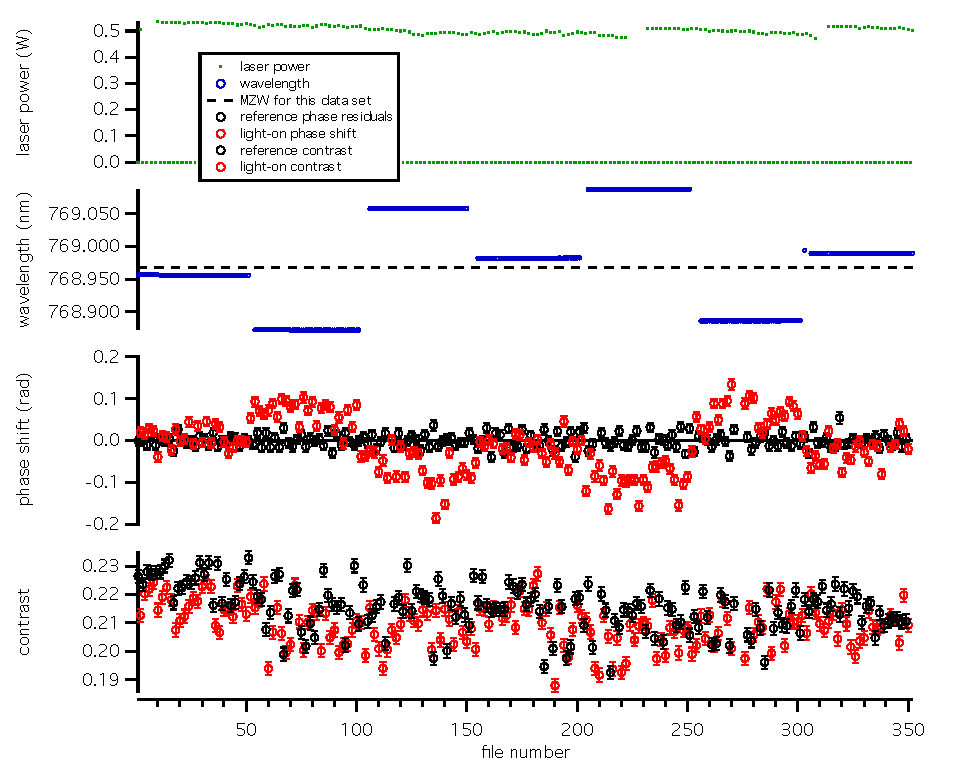
\includegraphics[width=.90\textwidth]{Figures/120509eRefOnPhaseWavePowerCon.pdf}}
\caption[Light-induced phase shift and contrast, and laser power and wavelength vs.~data file number]{\label{MZWRefOnPhase}Laser power, laser wavelength, reference atom interferometer phase residuals and contrast, and light-induced atom interferometer phase shift and contrast vs.~data file number. Each data point corresponds to 5 s of integration time. 29 out of 350 data points were deleted in this data set due to instabilities in either the laser power or wavelength during the 5 s integration time, and the phase shift data is ignored for these files. These deletions are accomplished using an unbiased and automated filter algorithm. These data are then further analyzed by normalizing the phase shift data by the laser power, and then binning and averaging the normalized phase shift data by wavelength, as shown in Figure \ref{MZWphaseVsWave}. The particular data shown here is data set 120509e.}
\end{figure}


After the initial data processing, we normalized the phase shift data by laser power to control for drifts of the tapered amplifier power and fiber coupling efficiency. In addition, polarization changes due to propagation through the fiber were converted to power instability by a polarizing beam splitter. The power-normalized phase shift data were then binned by wavelength, and the average, standard deviation, and standard error of the mean of the central 80\% of each bin was calculated. Figure \ref{MZWphaseVsWave} shows the resulting average power-normalized phase shift data vs.~wavelength. We performed a non-linear least-squares fit of this data to equation 4 from Appendix \ref{mzwAppendix} to determine the $\lambda_\textrm{zero}$ for each data series. For this fit, we weighted the normalized phase shift data by the standard error of the mean for each wavelength bin. The statistical error of each $\lambda_\textrm{zero}$ measurement was determined by the fit routine. The standard deviation is only shown for reference. The quality of fit shown in Figure \ref{MZWphaseVsWave} is typical of the entire data set. 


\begin{figure}
\centerline{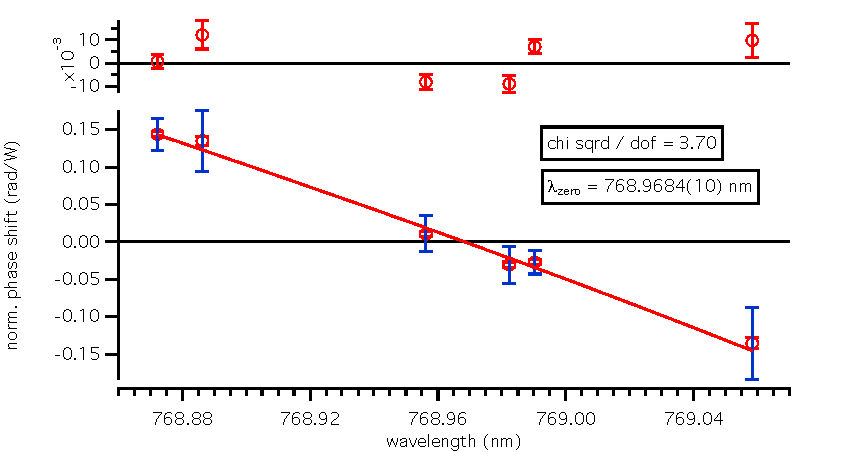
\includegraphics[width=.90\textwidth]{Figures/120509eMZWmeas.pdf}}
\caption[Power-normalized average phase shift vs.~wavelength for data series 120509e.]{\label{MZWphaseVsWave}Power-normalized average phase shift vs.~wavelength for data series 120509e. The red error bars are the standard error of the mean and the blue error bars are the standard deviation of the phase shifts measured at each wavelength. The 1.0 pm best-fit uncertainty of $\lambda_\textrm{zero}$ in this data series comes from $\chi^2$ minimization using input uncertainties of the standard error of the mean of the averaged phase shifts at each wavelength. The $\lambda_\textrm{zero}$ reported from this data series is compared to 34 other measurements each made in a similar way in Figure \ref{MZWmeasFig}.}
\end{figure}


Our reported $\lambda_\textrm{zero}$ measurement is the result of 35 individual measurements of $\lambda_\textrm{zero}$, such as the one shown in Figure \ref{MZWphaseVsWave}. Each $\lambda_\textrm{zero}$ measurement and an estimate of its statistical uncertainty is shown in Figure \ref{MZWmeasFig}. A histogram of the 35 measurements is shown in Figure \ref{MZWhistFig}. Note that these measurements have not been corrected for a constant Doppler shift of 0.56(5) pm. 


The reproducibility of the 35 $\lambda_\textrm{zero}$ measurements shown in Figure \ref{MZWmeasFig} is clearly much worse than the individual statistical errors. Furthermore, even the relative sizes of the individual statistical errors appear highly suspect since the reproducibility of the measurements i.e. the deviation from the mean, is uncorrelated with the size of the statistical errors. We therefore chose to assume that the statistical error of each data set was the same. We do not feel justified taking the weighted mean of these measurements because we do not believe the statistical errors associated with the each of the 35 individual measurements are accurate.


\begin{figure}
\centerline{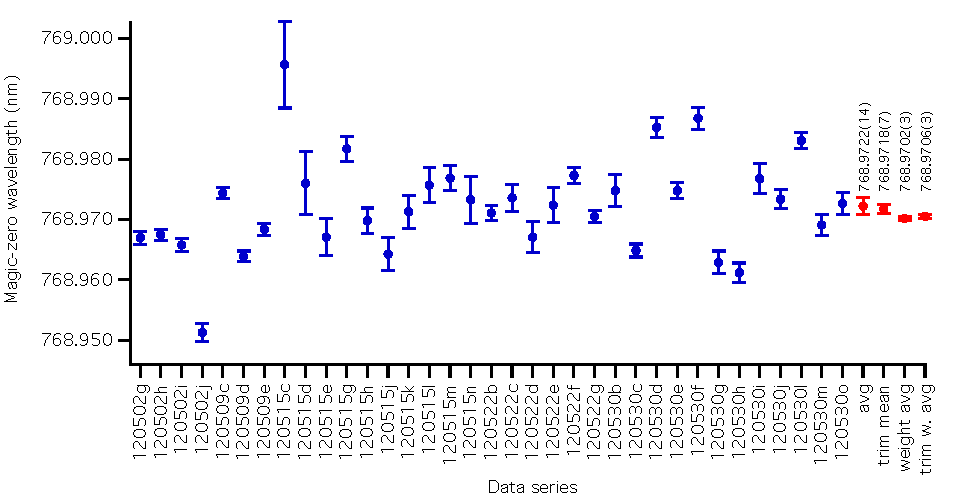
\includegraphics[width=.90\textwidth]{Figures/MZWmeasurements2.pdf}}
\caption[35 separate $\lambda_\textrm{zero}$ measurements and the average calculated in 4 different ways.]{\label{MZWmeasFig}35 separate $\lambda_\textrm{zero}$ measurements (blue) and the average calculated in 4 different ways (red). The overall average is $\lambda_\textrm{zero}=768.9722(14)$, the average of the central 80\% of the data is $\lambda_\textrm{zero}=768.9718(7)$ nm, the weighted overall average is $\lambda_\textrm{zero}=768.9702(3)$ nm, and the weighted average of the central 80\% of the data is $\lambda_\textrm{zero}=768.9706(3)$ nm. The error bars for each individual measurement show the uncertainty that was determined by $\chi^2$ minimization. However, as shown here, we found the experiment was not as reproducible as the reported individual measurement errors would suggest. Furthermore, the deviation from the mean was also uncorrelated with the size of the statistical error. Therefore, we assumed the statistical errors of all measurements were the same, and we report the standard error of the trimmed mean as the final statistical uncertainty. This data has not been corrected for a 0.56(5) pm Doppler shift. Figure \ref{MZWhistFig} shows a histogram of these data.}
\end{figure}


If we take the average of all 35 measurements and calculate the standard error of the mean, we find $\lambda_\textrm{zero}=768.9722(14)$ nm. Eliminating the highest and lowest 10\% of the data yields the reported measurement of $\lambda_\textrm{zero}=768.9718(7)$ nm (again, without the Doppler shift correction). The weighted average of all 35 points is $\lambda_\textrm{zero}=768.9702(3)$ nm, and the weighted average of the central 80\% of the data is $\lambda_\textrm{zero}=768.9706(3)$ nm. The statistical errors associated with the weighted averages are unrealistically small, yet, the central values are within 1.2 pm (2$\sigma$) of unweighted averages. 

\begin{figure}
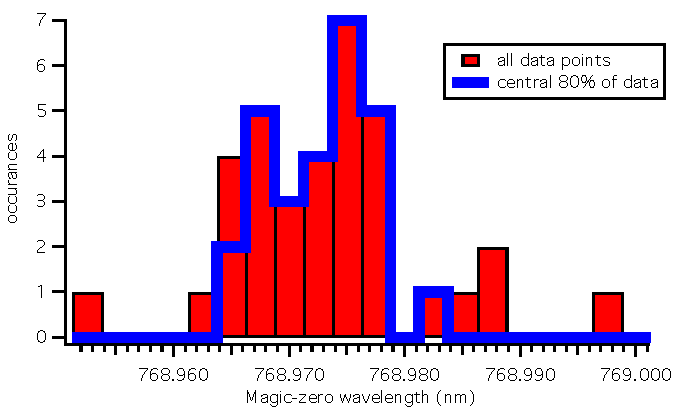
\includegraphics[width=.90\textwidth]{Figures/MZWhistogram.pdf}
\caption[Histogram of $\lambda_\textrm{zero}$ measurements.]{\label{MZWhistFig}Histogram of $\lambda_\textrm{zero}$ measurements. The central 80\%, used for the calculation of the trimmed mean, is highlighted in blue.}
\end{figure}





\section{Derivation of a fundamental limit for the sensitivity of a $\lambdaZero$ measurement}
\label{mzwLimitSection}
Decoherence due to spontaneous emission \cite{Cha95, Kok01a} limits the precision with which $\lambda_\textrm{zero}$ can be measured. The probability of an atom scattering zero photons, $P(0)$, affects the interferometer contrast through $C=C_0P(0)$, where $C_0$ is the reference contrast. Given a Poisson distribution for $P(0)$,
\begin{eqnarray}
\label{ceqn}
C = C_0 e^{-N(\omega)}
\end{eqnarray}
where $N(\omega)$ is the average number of photons an atom scatters while exposed to the laser beam with frequency $\omega$ for a time $T$. $N(\omega)$ is proportional to the time-averaged probability for atoms to be in an excited state, $P_{ex}$, and the decay rate $\Gamma$: 
\begin{eqnarray}
&N(\omega)=&P_{ex} T \Gamma.
\end{eqnarray}
When the excitation probability is much less than 1, and using the rotating wave approximation, we can write $P_{ex}$ in terms of the Rabi frequencies $\Omega_e=|\langle e | \bm{d} . \bm{\hat{\epsilon}} | g \rangle |E_0/\hbar$ and the detunings $\Delta_e$ from each resonance:
\begin{eqnarray}
\label{PexEqn}
P_{ex}=\frac{1}{2} \sum_e \frac{\Omega_e^2}{\Delta_e^2+\Omega_e^2}
\end{eqnarray}

The probability of an atom scattering 1 or more photons is $P_s=1-P(0)$. To obtain a simple expression for $P_s$ we make the approximation
\begin{eqnarray}
\label{P0eqnApprox}
P(0) \approx 1-N(\omega)
\end{eqnarray}
Using this approximation, we can write
\begin{eqnarray}
\label{psEqn}
P_s = N(\omega) = P_{ex}T\Gamma = T\Gamma \frac{1}{2} \sum_e \frac{\Omega_e^2}{\Delta_e^2+\Omega_e^2}.
\end{eqnarray}
To compare $P_s$ to the phase shift, we further assume $\Delta_e^2 \gg \Omega_e^2$ and rewrite $P_s$ as
\begin{eqnarray}
\label{psMatrixElEqn}
P_s = P_{ex}T\Gamma = \frac{I T\Gamma}{\epsilon_0 c \hbar^2} \sum_e \frac{|\langle e | \bm{d} . \bm{\hat{\epsilon}} | g \rangle |^2}{\Delta_e^2}.
\end{eqnarray}
In the rotating-wave approximation, the slope of the phase shift is
\begin{eqnarray}
\label{rwaPhaseDer}
\frac{d\phi}{d\omega}=\frac{IT}{2\epsilon_0c\hbar^2} \sum_e \frac{|\langle e | \bm{d} . \bm{\hat{\epsilon}} | g \rangle | ^2}{\Delta_e^2}.
\end{eqnarray}

Comparison of Eqs.~(\ref{rwaPhaseDer}) and (\ref{psMatrixElEqn}) yields a maximum achievable slope of
\begin{eqnarray}
\label{OmegaLimit}
\frac{d\phi}{d\omega}\approx\frac{1}{2\Gamma}P_s.
\end{eqnarray}
In terms of the wavelength, the slope is
\begin{eqnarray}
\label{LambdaLimit}
\frac{d\phi}{d\lambda}=\frac{d\phi}{d\omega}\frac{d\omega}{d\lambda}\approx\frac{\pi c P_s}{\lambda^2\Gamma}.
\end{eqnarray}

As discussed in Appendix \ref{mzwAppendix}, the highest sensitivity could be achieved if $P_0=e^{-1}$, implying an optimum $P_s=1-e^{-1}$. Given this requirement, we determine that the error made by the approximation in Eq.~(\ref{P0eqnApprox}) is $\approx30\%$. Still, the simple formulation of the maximum achievable slope presented in Eq.~(\ref{OmegaLimit}) remains a useful guide to possibility of large improvements in the precision of $\lambda_\textrm{zero}$ measurements. 




\section{Contrast loss due to inhomogeneous mechanisms}
\label{mzwContrast}

Although the phase shift is the primary signal in our measurement of $\lambda_\textrm{zero}$, it is still important to have a full understanding of the interferometer contrast loss. This provides a valuable check on our understanding of the potential errors associated with the measurement. Here we will examine three mechanisms of contrast loss, all analogous to inhomogenous broadening.

As stated in equation \ref{mzwIntEqn}, the phase acquired along one path in the atom interferometer is
\begin{eqnarray}
\label{inteqnEPAPS}
\phi_{0,q,|Fm_F\rangle}(\omega,x,v) = \frac{\alpha_{q,|Fm_F\rangle}(\omega)}{2\epsilon_0 c \hbar v}\int_{-\infty}^{\infty}I(x,z) dz.
\end{eqnarray}
Here we have written the phase as an explicit function of the atom wave position $x$, velocity $v$, light polarization $q$, and state $|Fm_F\rangle$ to more easily explain the contrast loss mechanisms. Next, we assume that the focused laser beam intensity distribution in the plane of the interferometer is represented by a Gaussian function
\begin{eqnarray}
\label{intensityEqnEPAPS}
I(x_l,z_l) = I_{0}e^{-2(x_l^2+z_l^2)/w_0^2}
\end{eqnarray}
where $w_0$ is the beam waist, $I_{0}=2P_L/(\pi w_0^2)$ and $P_L$ is the laser power. Integrating the acquired phase (Eq.~(\ref{inteqnEPAPS})) along the beam path ($z$) gives
\begin{eqnarray}
\label{nointeqniEPAPS}
\phi_{0,q,|Fm_F\rangle}(\omega,x,v) = \frac{\alpha_{q,|Fm_F\rangle}(\omega)\sqrt{\pi/2}w_0I_{0}}{2\epsilon_0 c \hbar v}e^{-2(x-x_l)^2/w_0^2},
\end{eqnarray}
or in terms of the laser power and beam waist
\begin{eqnarray}
\label{nointeqnpEPAPS}
\phi_{0,q,|Fm_F\rangle}(\omega,x,v)=\frac{\alpha_{q,|Fm_F\rangle}(\omega)P_L}{\sqrt{2\pi}\epsilon_0 c \hbar v w_0}e^{-2(x-x_l)^2/w_0^2}.
\end{eqnarray}


The differential phase shift between the two paths of the two interferometers formed by the +1 and 0, and the 0 and -1 diffraction orders is
\begin{subequations}
\label{diffPhaseEPAPS}
\begin{eqnarray}
\phi_{1,q,|Fm_F\rangle}(\omega,x,v) = \phi_{0,q,|Fm_F\rangle}(\omega,x+s(v),v)-\phi_{0,q,|Fm_F\rangle}(\omega,x,v)\\
\phi_{-1,q,|Fm_F\rangle}(\omega,x,v) = \phi_{0,q,|Fm_F\rangle}(\omega,x,v)-\phi_{0,q,|Fm_F\rangle}(\omega,x-s(v),v)
\end{eqnarray}
\end{subequations}
where $s(v)$ is the velocity-dependent path separation \cite{Hol10}. 


The velocity distribution in our supersonic atom beam is well-described by a Gaussian distribution
\begin{eqnarray}
\label{PveqnEPAPS}
P(v)=\frac{1}{\sqrt{2\pi\sigma_v^2}}\exp\left(-\frac{(v-v_0)^2}{2\sigma_v^2}\right)
\end{eqnarray}
where $v_0$ is the mean velocity and $\sigma_v$ is the velocity distribution width. In our experiment $v_0\approx1600$ m/s and $v_0/\sigma_v\approx15$.


Finally, we can predict the measured interferometer phase $\phi(\omega)$ and contrast $C(\omega)$ from the expression
\begin{eqnarray}
\label{cphiEPAPS}
C(\omega)e^{i\phi(\omega)}=C_0e^{i\phi_0}\sum_{q=-1,0,1}f_q\sum_{k=-1,1}\frac{1}{2}\sum_{|Fm_F\rangle}\frac{1}{8}\int_{v=0}^\infty P(v)\int_{x=-d/2}^{d/2}\nonumber\\
P(x)\exp(i\phi_{k,q,|Fm_F\rangle}(\omega,x,v)) dv dx.
\end{eqnarray}
Here, $f_q$ is the fraction of the power with $q$ polarization, typically $f_{0}=80\%$ and $f_{1}=20\%$. The factor of 1/2 accounts for equal detected intensity from the +1 and -1 interferometers. The factor of 1/8 accounts for the fact that all 8 $|Fm_F\rangle$ states are equally likely in our thermal atom beam. We also assume that the atom beam intensity $P(x)=1/d$ is uniform over the width $d$ of the detected fringes. Figure \ref{MZWcLossFig} shows contrast loss spectra based on Eq.~\ref{cphiEPAPS} with several conditions (e.g. zero beam width). Figure 1b in Appendix \ref{mzwAppendix} shows the same data and the calculated contrast loss spectra for the conditions $d=100$ $\mu$m, $\sigma_v=110$ m/s, $w_0=110$ $\mu$m. 


\begin{figure}
\centerline{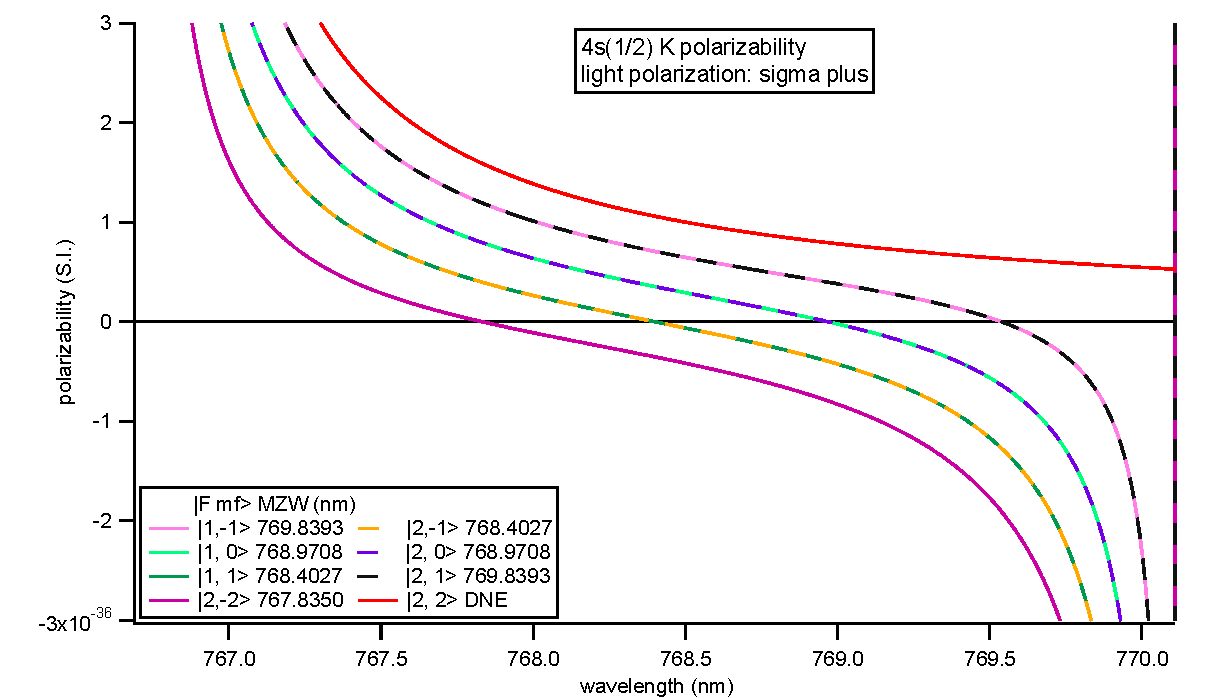
\includegraphics[width=.90\textwidth]{Figures/sigmaPlusMZW.pdf}}
\caption{\label{sigmaPlusMZW}Polarizabilities and magic-zero wavelengths for different $|Fm_F\rangle$ ground states of potassium for $\sigma^+$ light.}
\end{figure}


\begin{figure}
\centerline{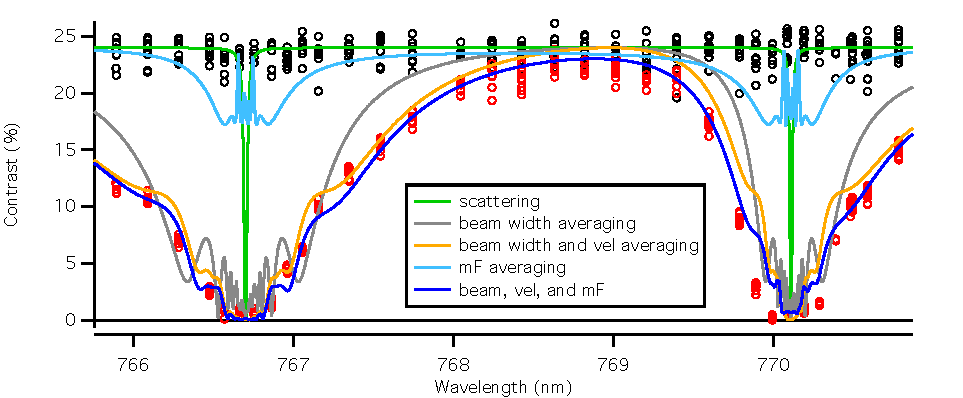
\includegraphics[width=1\textwidth]{Figures/cLossMechanisms.pdf}}
\caption[Interferometer contrast loss due to light between the potassium D1 and D2 lines.]{\label{MZWcLossFig}Measured interferometer reference contrast $C_0$ (black circles) and contrast $C$ when exposed to light (red circles). Also shown is predicted interferometer contrast loss due to averaging over the beam width only (grey line), the beam width and the velocity distribution (orange line), multiple $|Fm_F\rangle$ states only (light blue line), and all three of the above mechanisms (dark blue line). Contrast loss from photon scattering only is also shown (green line).}
\end{figure}



\section{The effect of broadband light on $\lambdaZero$ measurements}

We have assumed, until now, that the optical spectrum contains only one frequency of significance. Unfortunately, due to the nature of our laser system, this assumption is not valid. Our laser system consists of tunable a 50 mW external cavity diode laser seeding a 2 W tapered amplifier \cite{Haw01, Bol10, Nym06}. Tapered amplifiers are notorious for producing a significant amount of broadband spontaneous emission ($\sim10\%$ of the total power output) in addition to the amplified stimulated emission. Figure \ref{ASEgratingPic} shows a picture of the spectrum of the tapered amplifier power output after diffraction from a grating. Figure \ref{mzwSponData} shows data acquired with a grating spectrometer under different TPA conditions. Under normal operating conditions (40 mW of seed light and a TPA current of 2.6 A) the broadband light spectrum is consistent with a gaussian with a center wavelength of $\lambda_\textrm{spon}=763$ nm and a width of $\sigma_\textrm{spon}=3$ nm. Spontaneous emission from the tapered amplifier diverges at a different rate than the stimulated emission. We use this fact to reduce the fraction of spontaneous emission by an order of magnitude by spatially filtering the tapered amplifier output with a single mode fiber \cite{Voi01}. 


To account for the broadband light, the phase shift (equation \ref{mzwIntEqn}) becomes
\begin{eqnarray}
\label{mzwIntEqnASE}
\phi(\omega) = \frac{1}{\epsilon_0 c \hbar v} \int_{z=-\infty}^{\infty} \int_{\omega=0}^{\infty} \alpha(\omega)  I(\omega;x,z) dz d\omega.
\end{eqnarray}
Figure \ref{mzwSponSpectrum} shows a model of the broadband light spectrum with the dynamic polarizability near the potassium D1 and D2 lines.


\begin{figure}
\centerline{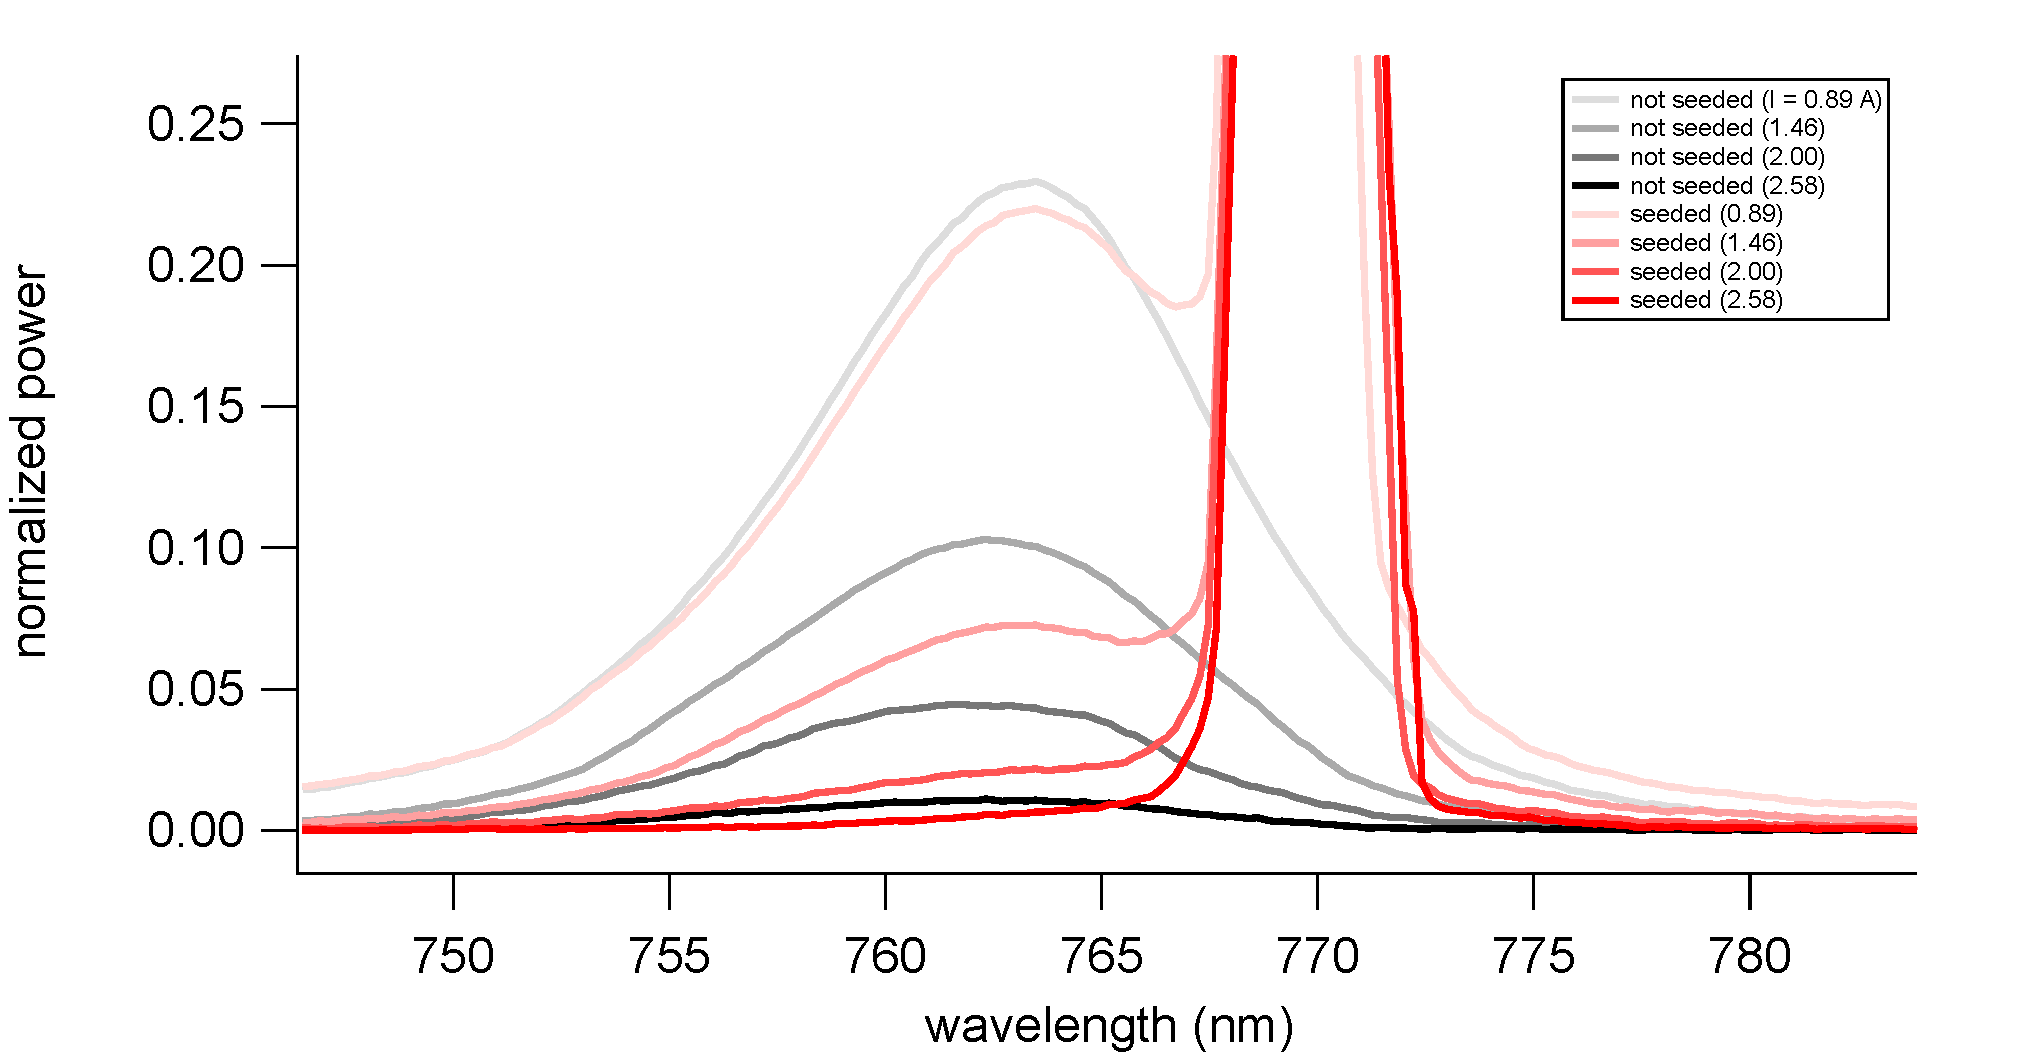
\includegraphics[width=.9\textwidth]{Figures/ASEdata.pdf}}
\caption[Laser spectrum measured with a grating spectrometer.]{\label{mzwSponData}Laser system spectrum before filtering by a single mode fiber for 4 different tapered amplifier injection currents: 0.89 A, 1.46 A, 2.00 A, and 2.58 A. Black curves are the unseeded tapered amplifier spectrum (spontaneous emission only). Red curves are the spectrum when the tapered amplifier is seeded. The darkness gradient corresponds to low (faint) to high (dark) currents. For each of the 4 currents, both the unseeded and seeded spectrum is normalized so that the maximum observed power is equal to 1. Thus it is evident that as the tapered amplifier injection current increases, the broadband light component decreases. The grating spectrometer resolution is approximately 0.3 nm, and this causes a blurring of the high power stimulated emission peak.}
\end{figure}


\begin{figure}
\centerline{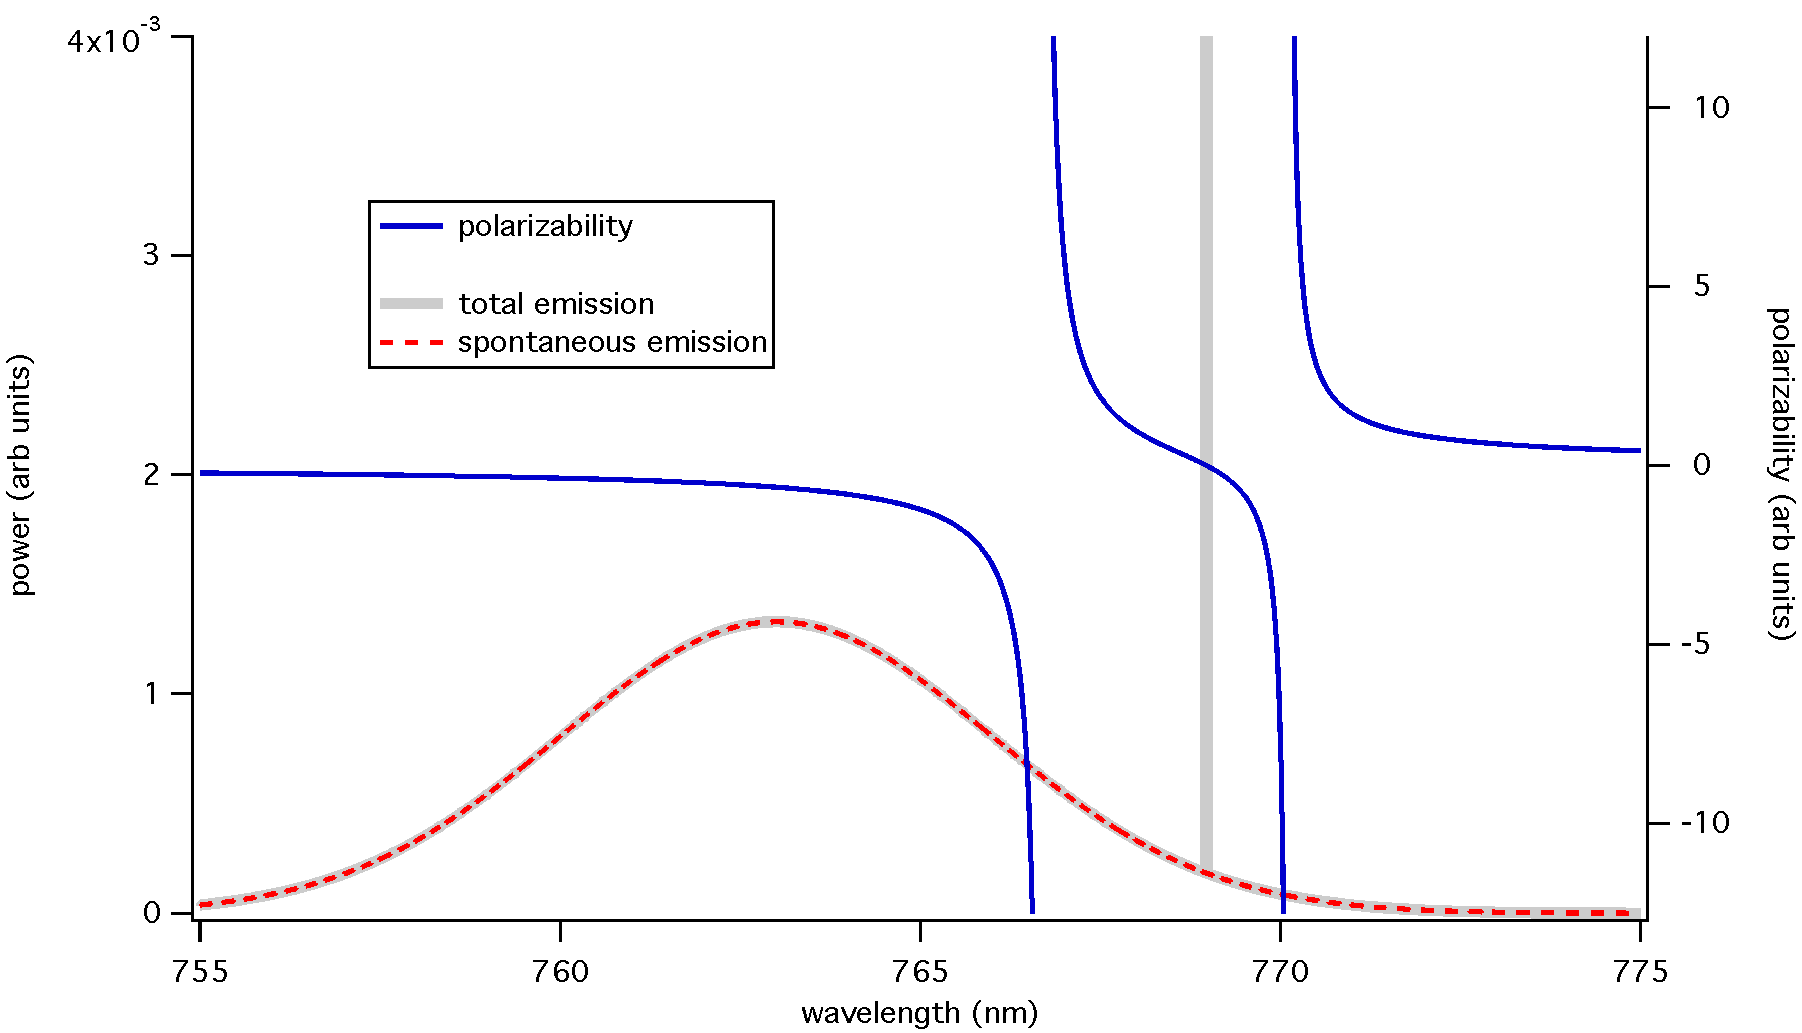
\includegraphics[width=.9\textwidth]{Figures/ASEmodelSpectrum2.pdf}}
\caption[Plot of the laser spectrum and the dynamic polarizability of potassium.]{\label{mzwSponSpectrum}Model of the laser system spectrum and the dynamic polarizability of K. The  broadband light component is set to be 1\% of the total laser power. The majority of the broadband light is blue-detuned of the D2 line, and thus there is a net phase shift due to the integrated spectral density of the broadband light.}
\end{figure}




%%%%%%%%%%%%%%%%%%%%%%%%%%%%%%%
\section{Next-generation $\lambdaZero$ measurements}
\label{mzwNextGenSec}
The existence of a $\lambdaZero$ near 770 nm in potassium was fortunate for our lab. We chose to study this particular $\lambdaZero$ for several reasons. First, potassium is cheap and easy to handle, and it is easy to generate and detect beams of potassium atoms in our lab. Second, the primary transitions are strong and the fine structure splitting of the $4p$ levels in potassium is only 3 nm, and this leads to a larger slope and thus easier to determine $\lambdaZero$. Third, inexpensive and easy-to-operate diode lasers and amplifiers are available near 770 nm.

Future measurements of magic-zero wavelengths in our lab will not have all of these advantages. Therefore, we are exploring ways to increase the light-induced phase shift in our atom interferometer and improve the reproducibility of the measurements. Three ideas to improve the signal size are a ``hall of mirrors" (Figure \ref{mzwHOM}), a power build-up cavity (Figure \ref{mzwCavityFig}), and a coaxial atom-light interaction region (Figure \ref{mzwHoleyMirror}). All of these ideas would rely on light delivered into the vacuum chamber by a single-mode optical fiber, and all optics would be rigidly attached to improve the stability and reproducibility of the experiment. 

We have already built a hall of mirrors and used it to measure the same $\lambdaZero$. The slope $d\phi/d\lambda$ is as much as 10 times larger as in our published experiment. Furthermore, the reproducibility during a single day is also improved and now consistent with the statistical error of a single $\lambdaZero$ measurement. We attribute this improvement in reproducibility to the increased mechanical robustness of the hall of mirrors system.

\begin{figure}
\centerline{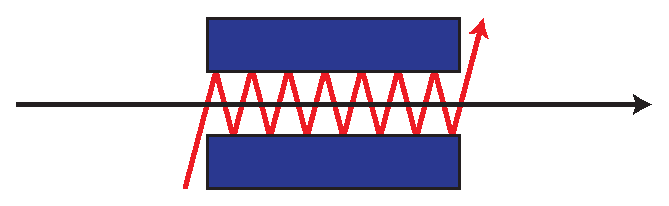
\includegraphics[width=.90\textwidth]{Figures/HOM.eps}}
\caption[A hall-of-mirrors for improved measurements of $\lambdaZero$.]{\label{mzwHOM}A ``hall-of-mirrors" for improved measurements of $\lambdaZero$. A hall-of-mirrors allows the laser beam to intersect the atom beam multiple times to create a larger phase shift. Nearly parallel mirrors and an appropriate choice of the focusing power of the lens may result in 30-50 times larger phase shifts.}
\end{figure}

\begin{figure}
\centerline{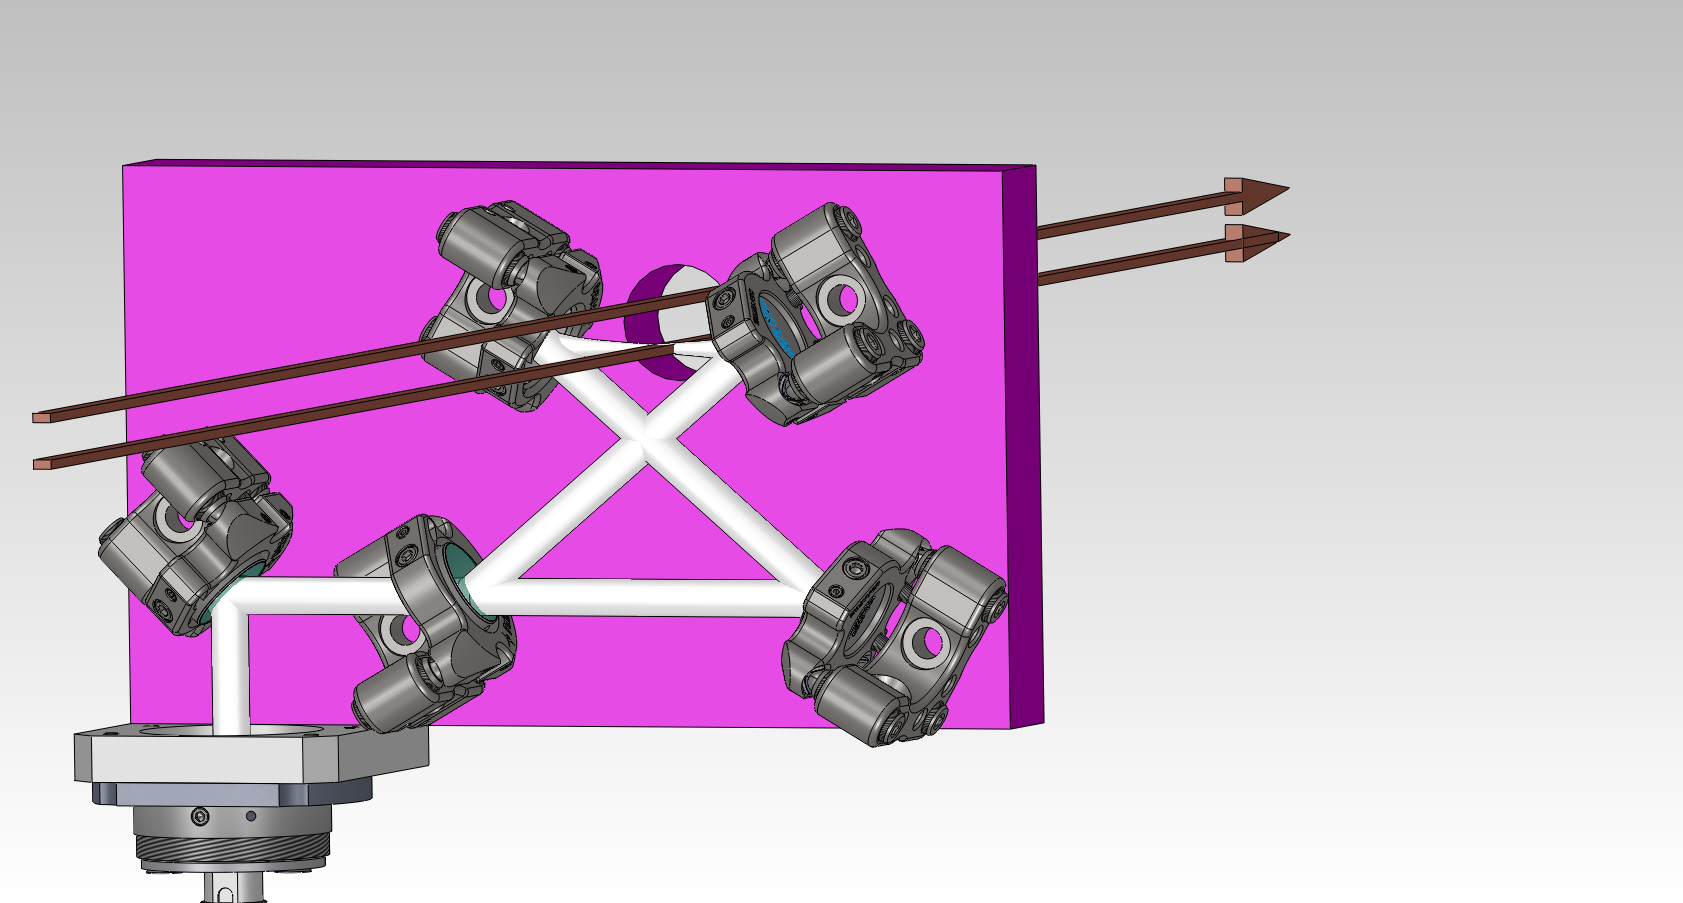
\includegraphics[width=.90\textwidth]{Figures/mzwCavityThruHole2.jpg}}
\caption[A power build-up cavity for improved measurements of $\lambdaZero$.]{\label{mzwCavityFig}A power build-up cavity for improved measurements of $\lambdaZero$. A power build-up cavity could provide 50-100 times larger phase shift for reasonable mirror reflectivities.}
\end{figure}

\begin{figure}
\centerline{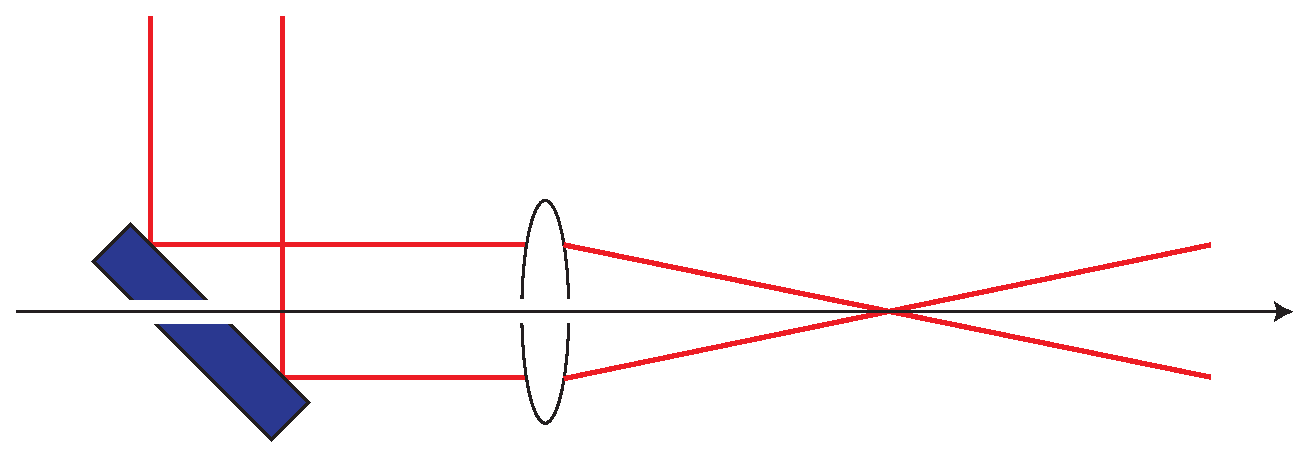
\includegraphics[width=.90\textwidth]{Figures/holeyMirror.eps}}
\caption[A coaxial atom-light interaction region for improved measurements of $\lambdaZero$.]{\label{mzwHoleyMirror}A coaxial atom-light interaction region for improved measurements of $\lambdaZero$. Light focused along the path of the atom beam could interact with the atoms for a significantly longer amount of time, leading to 50-100 times larger phase shifts. A small hole drilled in the mirror and lens would allow the atom beam to pass through while only reducing the total optical power by a few percent. The atoms would see significantly Doppler-shifted light, so an accurate measurement of the atom beam velocity is required in this system.}
\end{figure}



\chapter{STRONTIUM POLARIZABILITY MEASUREMENT PROPOSAL}
\label{alphaSrChapter}


\newcommand*{\sSz}{$^1\textrm{S}_0$~}
\newcommand*{\tPz}{$^3\textrm{P}_0$~}
\newcommand*{\tPo}{$^3\textrm{P}_1$~}
\newcommand*{\tPt}{$^3\textrm{P}_2$~}
\newcommand*{\sDt}{$^1\textrm{D}_2$~}
\newcommand*{\tDo}{$^3\textrm{D}_1$~}
\newcommand*{\sPo}{$^1\textrm{P}_1$~}
\newcommand*{\tSo}{$^3\textrm{S}_1$~}
\newcommand*{\muW}{$\mu\textrm{W}$~}

\newcommand*{\aSr}{$\alpha_\textrm{Sr}$}
\newcommand*{\aSrm}{$\alpha_\textrm{Sr*}$}


We propose to measure the strontium ground 5s$^2$ \sSz and metastable 5s5p \tPz polarizabilities to provide crucial tests of atomic structure calculations needed for next generation atomic clocks \cite{Mit10} and \cite{Lud08}. Due to uncertain polarizabilities of the clock states, the Sr and Yb clocks until recently had an uncertainty that is 70-250 times larger than their ultimate lifetime-limited precision \cite{Lud08, Lem09}. The polarizability influences the clock frequency because blackbody radiation from the thermal environment causes relatively large, uncertain Stark shifts of the clock states. Recent \emph{in situ} measurements of the differential polarizability of the clock states of Sr \cite{Mid12a} and Yb \cite{She12} have significantly reduced the uncertainties due to the BBR shift. However, measurements of the polarizabilities of the individual states are still in high demand due to the importance of accurate calibration of the BBR shift and due to the difficulty of calculating these polarizabilities.

In this chapter we will discuss in detail the three technical challenges of measuring \aSr~ and \aSrm:
\begin{itemize}
\item Detection of ground state Sr with resonant photoionization. 
\item Detection of metastable state Sr using resonant and non-resonant photoionization.
\item Metastable Sr generation using electron impact ionization.
\end{itemize}




\begin{figure}
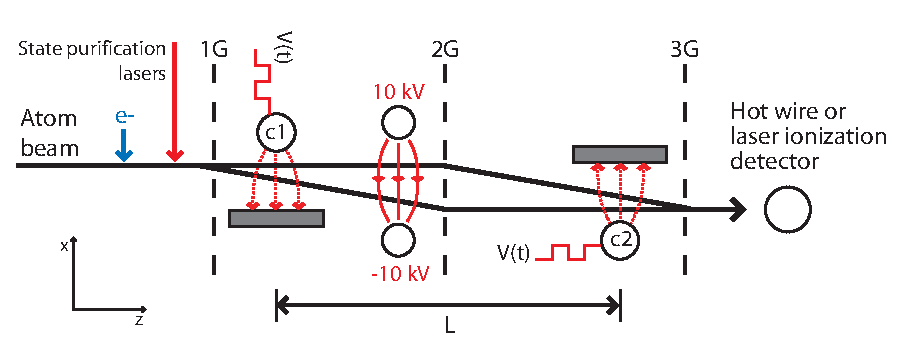
\includegraphics[width=1\textwidth]{Figures/IFMgradEfigNIST2011full.eps}
\caption[Atom interferometer configuration for strontium and ytterbium polarizability measurements.]{\label{IFMgradEfigSrYb}Atom interferometer set-up for strontium and ytterbium polarizability measurements. Nanogratings 1G, 2G, and 3G form a Mach-Zehnder atom interferometer. To measure beam velocity, we apply a periodic voltage $V(t)$ to two phase choppers (c1 and c2) separated by a distance $L$ and study the contrast of the interferometer as a function of switching frequency. To measure polarizability, we apply $\pm10$ kV across the interferometer to induce a polarizability-dependent phase shift. We will use an electron bombardment region to promote Sr and Yb atoms to a metastable state, followed by resonant lasers to purify the beam in the $^3\textrm{P}_0$ state. Beam detection will be accomplished with resonant laser ionization. Diagram not to scale.}
\end{figure}





%%%%%%%%%%%%%%%%%%%%%%%
\section{Detection of ground state Sr}

%%%%%
\subsection{Photoionization via 461 and 405 nm transitions}
The ionization energy of the ground 5s$^2$ \sSz state of strontium is 5.7 eV. This high ionization energy makes strontium difficult to ionize using our current hot-wire detector. We will discuss an efficient resonant photoionization pathway via a 461 nm photon to the 5s5p \sPo state and a 405 nm photon to the autoionizing state 5p$^2$ \sDt \cite{Men95,Van06,Haq07} (see Figure \ref{SrTerm}). We show that resonant photoionization will provide $\sim$20\% ionization probability with nearly zero background. We will assume that all lasers will be focused to a spot size of $A$=(100 $\mu\textrm{m})^2$ and that the atom beam velocity $v=3000$ m/s.

The \sSz- \sPo transition at 461 nm has an $A_{21}$ coefficient of $1.9\times10^8$ Hz. This corresponds to a state lifetime $\tau=5.3$ ns and $I_\textrm{sat}= 40$ mW/cm$^2$. Assuming a spot size of (100 $\mu\textrm{m})^2 =10^{-8}\textrm{ m}^2$, 4 $\mu\textrm{W}$ is needed to saturate this transition. The Rabi frequency $\Omega = \Gamma \sqrt{I/2I_{sat}}$ and for a two-state atom $\Gamma=A_{21}$. We will approximate the probability of finding a two-level atom in the excited state when $I=I_\textrm{sat}$ as $P\approx1/2$.


\begin{figure}
\centerline{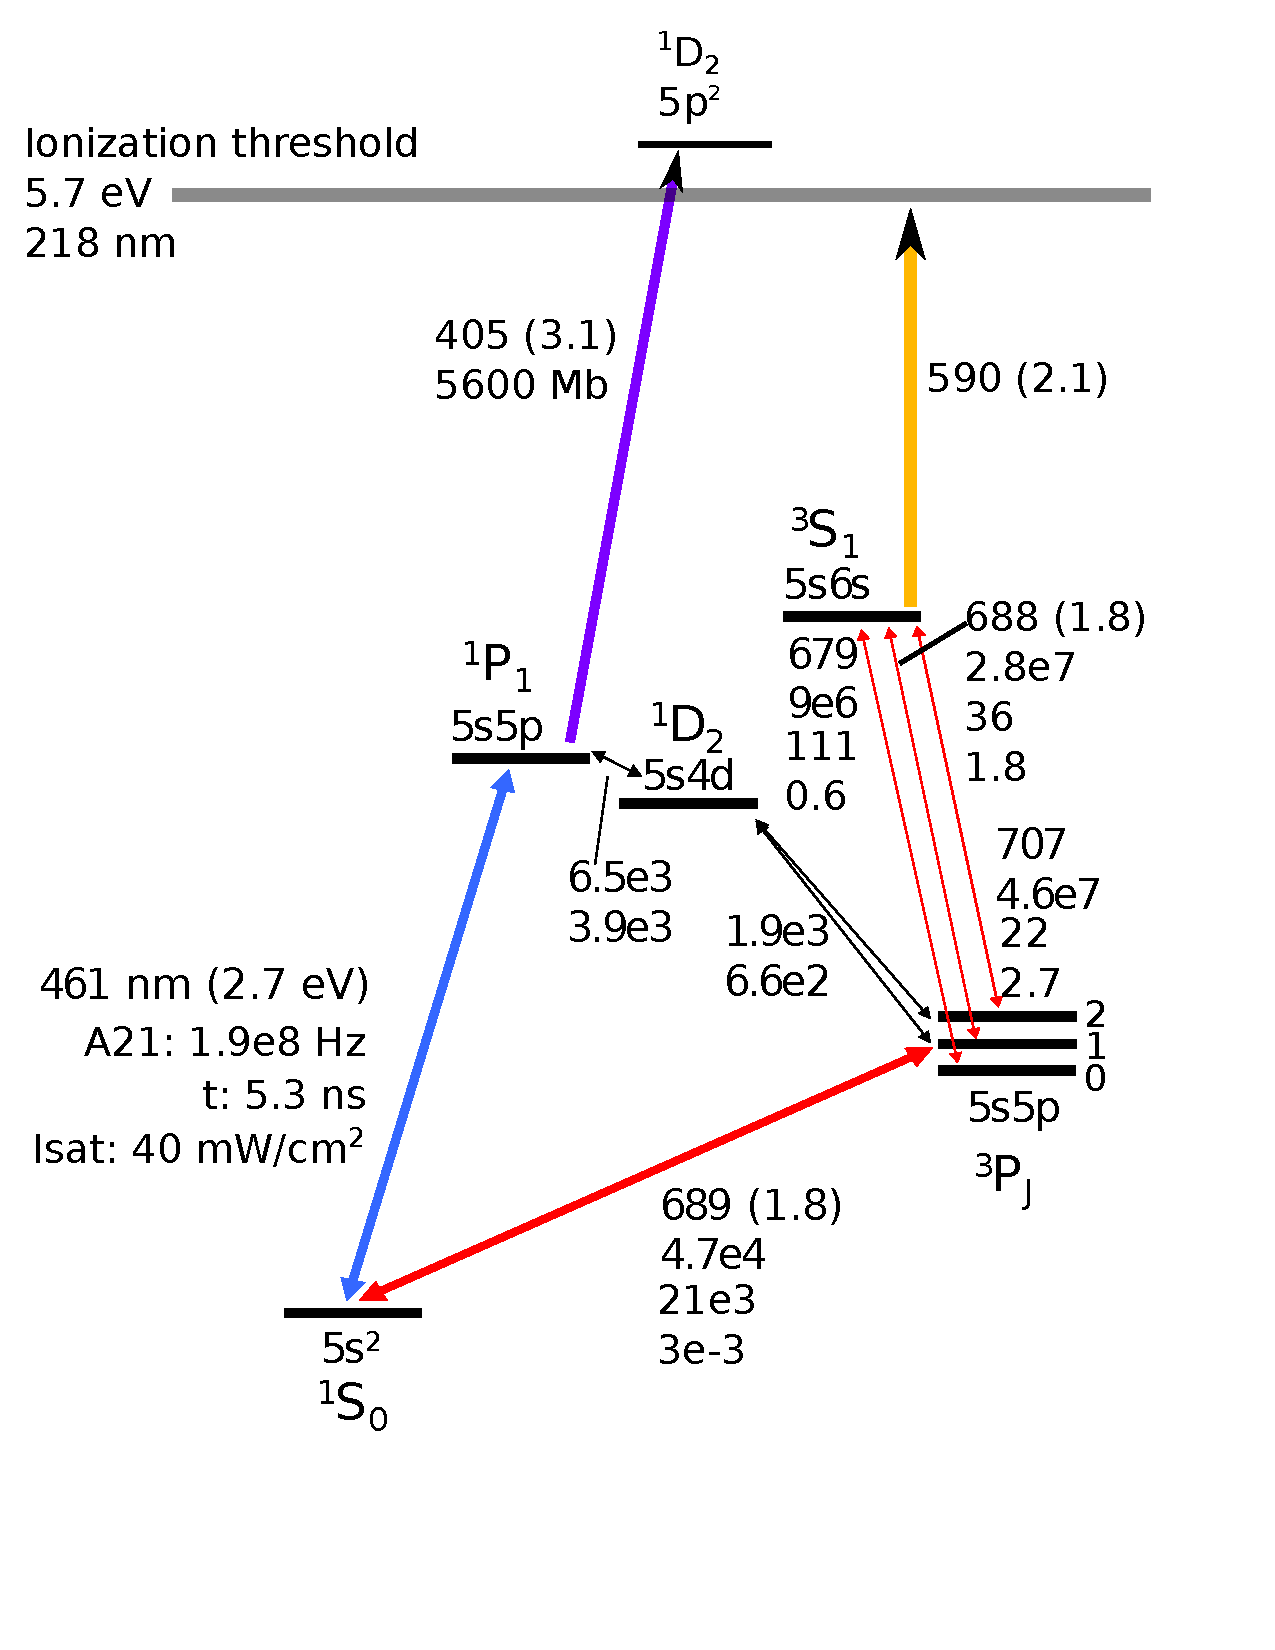
\includegraphics[scale=0.65]{Figures/LudlowSrDiagramMod.pdf}}
\caption[Strontium term diagram.]{\label{SrTerm}Sr term diagram. Transition wavelengths (nm), photon energies (eV), Einstein $A_{21}$ coefficients (Hz), lifetimes (ns), and $I_\textrm{sat}$ (mW/cm$^2$) are shown next to each transition. Adapted from Ludlow \cite{Lud08}. Note: $\Omega = \Gamma \sqrt{2I/I_{sat}}$.}
\end{figure}


Absorption of a 405 nm photon takes an atom in the excited 5s5p \sPo to the 5p$^2$ \sDt autoionizing state. The presence of this autoionizing state causes the ionization cross-section of the \sPo state with 405 nm light to be $10^3$ to $10^6$ times larger than typical non-resonant photoionization cross-sections: $\sigma=5600$ Mb (1 Mb = $10^{-22}$ m$^2$). 


We will now calculate the ionization probability a strontium atom in the ground state via this resonant ionization path. First, we write the single atom ionization rate from the \sPo state as 
\begin{eqnarray}
\Gamma_{1\textrm{P}1-\textrm{Sr}^+} = \sigma\Phi_\gamma = \sigma \frac{I_{405}}{E_\gamma} 
\end{eqnarray}
where $\sigma$ is the ionization cross-section, $\Phi_\gamma$ is the 405 nm photon flux, $I_{405}$ is the laser intensity for a beam with power $P_{405}$ focused to a spot size $A$, and $E_\gamma=hc/\lambda$ is the photon energy. We calculate $\Gamma_{1\textrm{P}1-\textrm{Sr}^+} = 10^7$ s$^{-1}$, assuming $P_{405}=100$ mW and A=(100 $\mu\textrm{m})^2$. Next, we must consider the time that the atom beam interacts with the ionization laser: $T=l/v$, where $l=\sqrt{A}$ is the interaction length. $T=30$ ns, assuming a beam velocity of 3000 m/s. The probability of photoionization from the \sPo state is then
\begin{eqnarray}
\textrm{Prob}_{1\textrm{P}1-\textrm{Sr}^+} = \Gamma_{1\textrm{P}1-\textrm{Sr}^+} T = \sigma \frac{P}{E_\gamma v \sqrt{A}}.
\end{eqnarray}
Using the above assumptions, we calculate an ionization probability of 38\% from the \sPo state. We assume that the intensity of light resonant with the \sSz - \sPo transition is sufficient to put atoms in the \sPo state 50\% of the time, and then estimate the ground state ionization probability of our system to be $\textrm{Prob}_{1\textrm{S}0-\textrm{Sr}^+}=10-20\%$. 


This resonant photoionization detection efficiency is comparable to our hot-wire detector efficiency with potassium, rubidium, and cesium atoms. However, the resonant photoionization method will presumably have a much lower noise floor than the hot-wire method. Therefore, we can expect that resonant photoionization will work for our system even if our ionization probability estimates are off by several orders of magnitude.



%%%%%%
\subsection{Generating 461 and 405 nm light}
Several possibilities exist for generating 461 nm light: frequency doubling 922 nm light, a blue LED, a strontium hollow cathode lamp, and an AR-coated laser diode.


First, we discuss second harmonic generation of 461 nm light. The efficiency of SHG of 922 nm to 461 nm varies from 0.01-75\% \cite{Van06,Tar05} depending on the effort expended, expertise of the lab, cavity specifications, and type of crystal used. A PPKTP crystal can achieve 1\% conversion efficiency with a single pass through the crystal when pumped with about 100 mW of 992 nm light, so no cavity would be needed. This may yield sufficient power and would be relatively simple. The crystal would need to be temperature tuned to 40-70 $^\circ$C. We estimate that it is reasonable that 100 \muW of resonant 461 nm light may delivered to the beam using SHG with a PPKTP. A prototype in our lab using a PPKTP crystal currently outputs about 10 \muW of 461 nm light.


We also explored several other methods to generate 461 nm light. Blue LEDs with center wavelengths near 460 nm provide another possibility for generating 461 nm light. LEDs with optical powers of 1 W are available. The typical $\Delta\lambda=25$ nm, corresponding to a frequency dispersion of $df=c/\lambda^2d\lambda=3\times10^{13}$ Hz. The linewidth of the \sSz-\sPo transition is 30 MHz, so approximately $10^{-6}$ of the light generated in the LED, 0.1-1 $\mu$W, may be resonant with the atom beam. 


Hollow cathode lamps are typically specified as producing 10-20 mA discharge current, however, the corresponding optical power is unknown. Typical operating voltages are 300 V. We assume an optical output power $P$, and that owing to the extended nature of the source, only 10\% of the light may be delivered to the atom beam. The doppler-broadening of the light from a hollow cathode lamp will further reduce the effective power. We assume a temperature of 900 K and calculate a corresponding doppler width of 1.5 GHz. The linewidth of the \sSz-\sPo transition is 30 MHz, so approximately 2\% of the light generated in the lamp may be resonant with the atom beam. The above factors yield an efficiency of $0.002P$. Hollow cathode lamps are relatively inexpensive (\$355), and require a 550 V, 20 mA power supply (available for \$2125, although we have a supply that would probably work). Hollow cathode lamp lifetimes are warranted to 5000 mA hours. At 10 mA, the lifetime would be 500 hours, or about 20 days of continuous operation. This can be quickly implemented with little expertise, and may provide sufficient power. 


Finally, Shimada \etal recently used a prototype AR coated diode from Nichia to generate 40 mW at 461 nm from an ECDL \cite{Shi13}. Commercialization of this diode technology would greatly simplify our strontium polarizability measurement.





%%%%%%%%%%%%%%%%%%%%%%%
\section{Detection of metastable Sr}


We now consider photoionization of the metastable \tPz state. To our knowledge, no autoionizing triplet states exist, so non-resonant photoionization must be used with the metastable state. The ionization energy of the \tPz state is 3.9 eV (318 nm). Therefore, direct photoionization of the \tPz state would require an intense UV source. The near-threshold photoionization cross-section of the \tPo state is $\sigma_{3P1}\approx 10$ Mb \cite{Haq07}. A UV lamp may provide sufficient power at this wavelength to directly ionize the \tPz state. Wang \cite{Wan11} used a UV LED to photoionize \tPz Ba atoms. We are exploring if we can use UV light to photoionize the \tPz with sufficient efficiency. UV LEDs with 0.5 mW available for $\sim$\$150. High power (0.5 W) UV LEDs are common down to 365 nm.

We also considered the possibility of using a two photon ionization process via the 5s5p \tPz to 5s6s \tSo at 679 nm (1.8 eV), and then an ionizing photon with $\lambda<590$ nm (2.1 eV). To our knowledge, no published photoionization cross-sections exist for the 5s6s \tSo state. Therefore, we estimate that the photoionization cross-section for the \tSo state is similar to that of the 5s6s \sSz state: $\sigma_{1S0}=0.4$ Mb \cite{Sam06}. \tSo will also decay to \tPo and \tPt, so we must apply the state purification lasers at detector as well to keep atoms in the \tSo state.

Another possible intermediate state is 5p$^2$ $^3\textrm{P}_1$. The transition between 5s5p \tPz and 5p$^2$ \tPo is at 474 nm (2.6 eV). The transition rate is $4\times10^7$ Hz \cite{Por08}. A photon with $\lambda< 950$ nm (1.31 eV) would be needed to photoionize the 5p$^2$ \tPo state. 473 nm diodes with several 10s of mW are available from several sources, including ThorLabs.

Yet another possible intermediate state is 5s5d \tDo. The transition between 5s5p \tPz and 5s5d \tDo is at 483 nm (2.6 eV). The transition rate is $4\times10^7$ Hz \cite{Por08}. A photon with $\lambda< 915$ nm (1.35 eV) would be needed to photoionize the 5s5d \tDo state. 490 nm diodes with several 10s of mW are available from several sources (Renesas NX6414EH, CrystaLaser, ThorLabs).




\section{Generating metastable Sr}

Metastable strontium and ytterbium will be generated in an electron bombardment region \cite{Giu88} and state purification will be accomplished with resonant lasers. The electron bombardment region will populate the nsnp$^3$P metastable triplets with 40\% efficiency. We will build diode lasers at 679 and 707 nm to optically pump metastable strontium atoms from the $^3\textrm{P}_1$ and $^3\textrm{P}_2$ states into the $^3\textrm{P}_0$ state. We will also build diode lasers at 649 and 770 nm to purify the ytterbium metastable triplet. We have prototypes of two of these lasers (679 and 770 nm) available from experiments with lithium and potassium atoms.





\chapter{TENSOR POLARIZABILITY MEASUREMENT PROPOSAL}
\label{dimersChapter}


%Do calculations for K$_2$, Rb$_2$, and Cs$_2$, and make corresponding edits.

Ground-state alkali atoms are spherically symmetric, and as a result the polarizability may be described by a scalar that does not depend on the direction of the applied field. In contrast, molecules are generally not spherically symmetric and their polarizabilities must be described by a tensor $\tensorPol$. Knowledge of the tensor polarizabilities of alkali dimers is currently of interest for ultracold molecules \cite{Dei08a}. Figure \ref{dimerOrientationFig} shows the two unique orientations of an alkali dimer in an electric field. To our knowledge, only the average polarizability of this tensor has been measured \cite{Tar93,Mol74}. 

M.S.~Chapman first proposed to measure the tensor polarizability of Na$_2$ by studying interferometer contrast loss as a function of applied electric field but dismissed the idea in favor of applying orthogonal electric fields to two well-separated paths of a molecule interferometer \cite{Cha95Thesis}. While there is significant merit to the orthogonal field approach, a separated path molecule interferometer even for Na$_2$ is a formidable challenge, and becomes more difficult for heavier atoms. Here, we examine in more detail the possibility of determining the tensor components of the molecular polarizability of alkali dimers by studying the unique contrast loss signal in our interferometer as a function of the applied electric field. 

The Stark shift of a molecule with a tensor polarizability $\tensorPol$ is given by 
\begin{eqnarray}
U=-\frac{1}{2} \vec{E} \tensorPol \vec{E}.
\end{eqnarray}
In general, the polarizability tensor is most easily expressed in the body coordinates of the molecule.  For a simple molecule such as an alkali dimer, the tensor is diagonal if one chooses to use the obvious axes of symmetry: one along the bonding axis of the molecule and two additional axes that are mutually orthogonal to the bonding axis. If we let the z-axis coincide with the bonding axis of the dimer we can write the polarizability tensor as
\begin{eqnarray}
\tensorPol = 
	\begin{pmatrix}
		\alpha_\perp	&		0		&		0		\\
			0		&	\alpha_\perp	&		0		\\
			0		&		0		&	\alpha_{||}		\\
	\end{pmatrix}
\end{eqnarray}
Let the average polarizability of the molecule be defined as
\begin{eqnarray}
\alpha = \frac{\alpha_{||}+2\alpha_\perp}{3} 
\end{eqnarray}
and let the anisotropy be defined as
\begin{eqnarray}
\gamma = \alpha_{||} - \alpha_\perp.
\end{eqnarray}

We transform the electric field from the lab coordinate system into the body coordinate system to calculate the energy shift. From symmetry we expect that the energy can only depend on the polar angle $\theta$. Let the electric field in the lab coordinate system be coincident with the lab z-axis. Following the standard coordinate system transformation matrices \cite{Gol02} we find
\begin{eqnarray}
\vec{E}_\textrm{body} &=& 
	\begin{pmatrix}
		\cos(\psi)		&	\sin(\psi)		&		0		\\
		-\sin(\psi)		&	\cos(\psi)		&		0		\\
			0		&		0		&		1		\\
	\end{pmatrix}
	\begin{pmatrix}
			1		&		0		&		0		\\
			0		&	\cos(\theta)	&	\sin(\theta)	\\
			0		&	-\sin(\theta)	&	\cos(\theta)	\\
	\end{pmatrix}
	\begin{pmatrix}
		\cos(\phi)		&	\sin(\phi)		&		0		\\
		-\sin(\phi)		&	\cos(\phi)		&		0		\\
			0		&		0		&		1		\\
	\end{pmatrix}
	\begin{pmatrix}
			0	\\
			0	\\
			E	\\
	\end{pmatrix}
	\nonumber \\
	&=& E
	\begin{pmatrix}
			\sin(\psi)\sin(\theta)	\\
			\cos(\psi)\sin(\theta)	\\
			\cos(\theta)	\\
	\end{pmatrix}
\end{eqnarray}
 

We may now calculate the energy shift
\begin{eqnarray}
U = -\frac{1}{2}E^2\left(\alpha_{||}-\gamma\sin^2\theta \right).
\end{eqnarray}
We assume that a uniform electric field is applied to one path of the interferometer for a distance $l$. The interaction phase shift is then
\begin{eqnarray}
\phi(E,\theta,v) 	&=& -\frac{1}{\hbar v} \int U dx  \nonumber \\
			&=& \frac{E^2 l}{2\hbar v}\left(\alpha_{||}-\gamma\sin^2\theta \right)
\end{eqnarray}
where $v$ is the velocity of the molecule.

The phase shift of the measured interference fringe will be an incoherent sum of the phase shifts of molecules with a random spatial orientation. Additionally, we must the average the phase shifts of the velocity distribution, $P(v)$. The measured contrast $C_m$ and phase shift $\phi_m$ will be
\begin{eqnarray}
C_m\exp(i\phi_m) = \int_{\theta=0}^\pi \int_{v=0}^\infty \exp(i\phi(E,\theta,v))P(v) \sin(\theta) d\theta dv.
\end{eqnarray}

The incoherent sum of fringes formed by molecules with different spatial orientations leads to contrast loss and revivals. The revivals occur when the phase shift corresponding to $\alpha_\perp$ is an integer multiple of $2\pi$ times the phase shift corresponding to $\alpha_{||}$. The velocity distribution only leads to contrast loss. Figure \ref{molConVelGamma} shows contrast loss due to these two different mechanisms for Na$_2$ molecules and the contrast loss due to both mechanisms combined for two different velocity distributions. Here, the velocity distribution width is parameterized by the sharpness $r=v_0/\sigma_v$. 
\begin{figure}
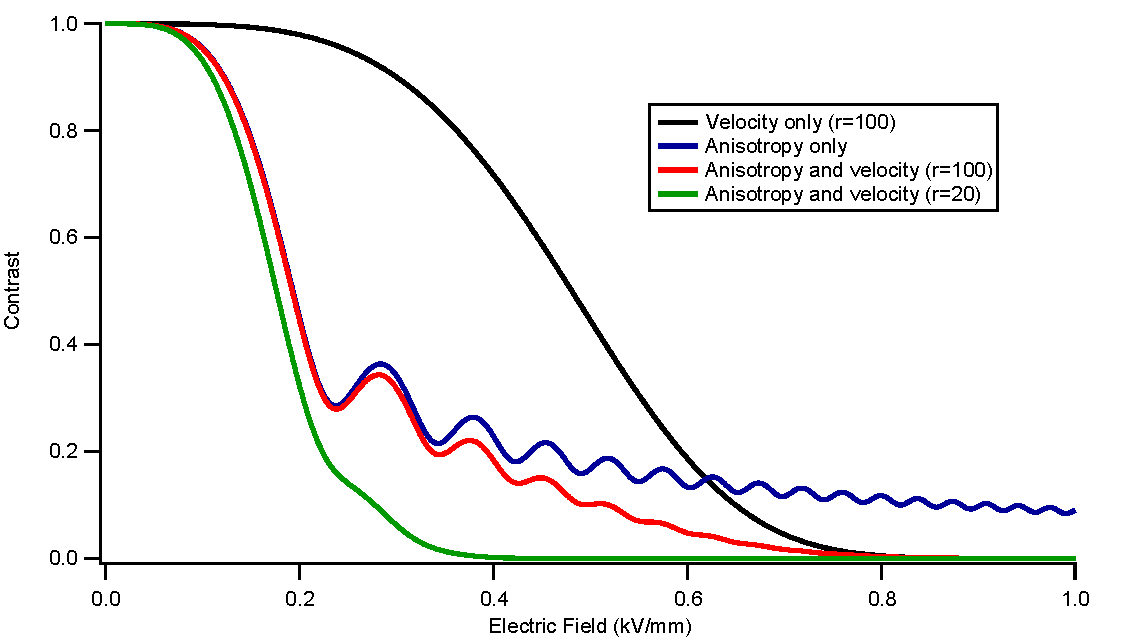
\includegraphics[width=1\textwidth]{Figures/molConVelAndGamma3.pdf}
\caption[Contrast loss due to tensor anisotropy for Na$_2$ molecules]{\label{molConVelGamma}Contrast loss due to anisotropy, velocity distribution, and both mechanisms combined for Na$_2$ molecules. A velocity distribution with a sharpness better than $r=v_0/\sigma_v > 20$ is necessary to see the effect of anisotropy on the contrast loss signal.}
\end{figure}
%
%\begin{figure}
%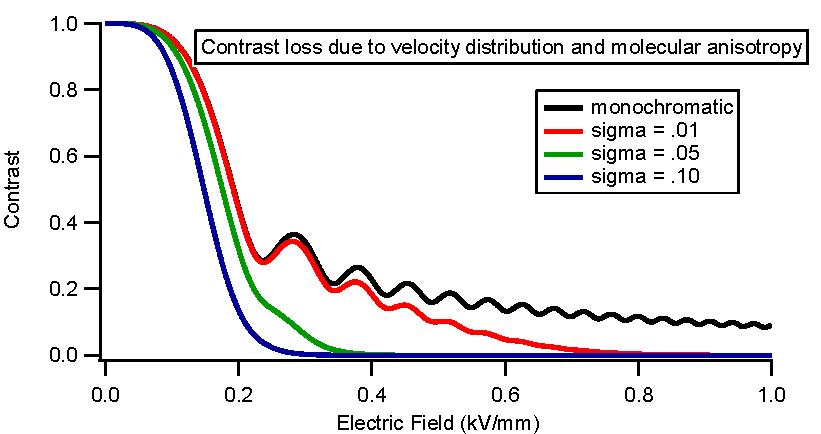
\includegraphics[width=1\textwidth]{Figures/molConSigmas.pdf}
%\caption{\label{molConSigmas}Contrast loss for different velocity distributions.}
%\end{figure}

A velocity distribution with a sharpness $r> 20$ is necessary to see the effect of anisotropy on the contrast loss signal. Alternatively, we could apply a counter-phase to reverse the contrast loss due to the velocity distribution at a given phase \cite{Rob04,Rob02}. We routinely observe velocity distributions sharper than 20, and even as large as 45 for Cs atoms. Significant experimental challenges include generating a bright enough molecule beam and eliminating the atomic component of the beam. It would also be interesting to consider the signal from a planar molecule such as benzene if a suitable detector (such as an electron impact ionizer) could be developed.




\chapter{CONCLUSIONS AND OUTLOOK}
\label{conclusions}

We began this thesis by asking: what happens to an atom in an electric field? The work described here answered this question with unprecedented precision. We measured the static polarizability of potassium and rubidium with 0.5\% uncertainty, and measured polarizability ratios with 0.3\% precision. We measured a magic-zero wavelength of potassium -- the wavelength at which nothing happens to the atom in the electric field -- for the first time. We also developed a new atom beam velocity measurement technique, phase choppers, to enable even more precise polarizability measurements in the future. 

Looking forward, we can realistically anticipate improved measurements of static polarizabilities and magic-zero wavelengths in the Cronin lab. The experiments described in this thesis form the foundation of a long program of static and dynamic polarizability measurements in Arizona. At this time, new measurements of cesium, strontium, and ytterbium polarizabilities appear to be of the highest importance. We have already measured the polarizability of Cs with 0.1\% precision (Figure \ref{csPolNew}). We have also generated beams of Sr and Ba, as well as beams of metastable He and Ar. Preliminary results using a hall-of-mirrors interaction region have shown a 5-10 times increase in the precision of $\lambdaZero$ measurements.

Have we answered the question of what happens to an atom in an electric field well enough? What will we learn by continuing to improve upon polarizability and magic-zero wavelength measurements?

We believe that there is significant value in pursuing improved measurements of static and dynamic polarizability. Table \ref{polResultsRecValues} showed the state-of-the-art measurements and calculations of the static polarizabilities of the alkalis. Theory uncertainty is currently about a factor of 2-5 better than the experiment uncertainty for most of these atoms, but theory uncertainty is difficult to estimate and theorists still routinely request new benchmark measurements of polarizabilities. New experiments are underway to probe parity non-conservation in Cs and Yb, and these experiments will need higher precision measurements of polarizabilities to test the associated atomic structure calculations. Next-generation optical clocks also need higher precision measurements of polarizabilities to accurately correct for blackbody radiation shifts in the clock frequencies. 

Future measurements of magic-zero wavelengths will determine difficult-to-calculate matrix elements with high precision, and may provide a sensitive way to probe the core electron contribution to polarizabilities. The many-body physics involved in the calculation of core electron polarizabilities has wide applications in atomic, nuclear, and condensed matter physics.

Polarizability, magic-zero wavelength, and van der Waals potential measurements of small molecules will have applications ranging from testing density functional theory to nanotechnology. We are currently working on implementing an electron ionization detector and mass filter to enable these measurements with molecules and non-alkali atoms.

Finally, it is worthwhile to reflect on the fact that when the Bederson group started its polarizability measurement program in the early 1960s there were no proposals to measure parity non-conservation in atomic systems (although the idea had been considered and dismissed as impractical \cite{Der07}) nor had atomic clocks been built with such incredible precision that blackbody radiation became an important component in the error budget. However, the Bederson group recognized the wide applications of polarizability measurements and their utility as benchmarks for the rapidly growing field of atomic physics. Similarly, future atomic physics experiments may well benefit from our measurements of polarizabilities today.





% Include the various appendices
\appendix
\chapter{REPRINT: ABSOLUTE AND RATIO MEASUREMENTS OF THE POLARIZABILITY OF NA, K, AND RB WITH AN ATOM INTERFEROMETER}
\label{polPRAappendix}
The following manuscript was published as a peer-reviewed article in Physical Review A. The results of this article are summarized in section \ref{polBrief} and Chapter \ref{polChapter} provides supplementary information. The manuscript is reprinted with permission from the American Physical Society. Original reference: W. F. Holmgren, M. C. Revelle, V. P. A. Lonij, and A. D. Cronin, ``\emph{Absolute and ratio measurements of the polarizability of Na, K, and Rb with an atom interferometer}", Physical Review A $\mathbf{81}$, 053607, (2010). Copyright (2010) by the American Physical Society.

\newcommand{\figPRA}[1]{
\begin{figure}
\includegraphics[ viewport= 50 30 560 770, width=.95\textwidth,clip]{Hol10PRA/#1}
\end{figure}
} 


\figPRA{pg1}
\figPRA{pg2}
\figPRA{pg3}
\figPRA{pg4}
\figPRA{pg5}
\figPRA{pg6}
\figPRA{pg7}
\chapter{REPRINT: ATOM BEAM VELOCITY MEASUREMENTS USING PHASE CHOPPERS}
\label{choppersAppendix}
The following manuscript was published as a peer-reviewed article in the New Journal of Physics. The results of this article are discussed in section \ref{choppersBrief} and Chapter \ref{choppersChapter} provides supplementary information. The manuscript is reprinted with permission from IOP Publishing Ltd. Original reference: W. F. Holmgren, I. Hromada, C. E. Klauss, and A.D. Cronin, ``\emph{Atom beam velocity measurements using phase choppers}", New Journal of Physics $\mathbf{13}$, 115007, (2011). Copyright (2011) by IOP Publishing Ltd.



\newcommand{\figNJP}[1]{
\begin{figure}
\includegraphics[ viewport= 50 30 560 770, width=.95\textwidth,clip]{Hol11NJP/#1}
\end{figure}
} 


\figNJP{pg1}
\figNJP{pg2}
\figNJP{pg3}
\figNJP{pg4}
\figNJP{pg5}
\figNJP{pg6}
\figNJP{pg7}
\figNJP{pg8}
\figNJP{pg9}
\figNJP{pg10}
\chapter{REPRINT: MEASUREMENT OF A WAVELENGTH OF LIGHT FOR WHICH THE ENERGY SHIFT FOR AN ATOM VANISHES}
\label{mzwAppendix}
The following manuscript was published as a peer-reviewed article in Physical Review Letters. The results of this article are discussed in section \ref{mzwBrief} and Chapter \ref{mzwChapter} provides supplementary information. The manuscript is reprinted with permission from the American Physical Society. Original reference: W. F. Holmgren, R. Trubko, I. Hromada, and A. D. Cronin, ``\emph{Measurement of a Wavelength of Light for Which the Energy Shift for an Atom Vanishes}", Physical Review Letters $\mathbf{109}$, 243004, (2012). Copyright (2012) by the American Physical Society.


\newcommand{\figPRL}[1]{
\begin{figure}
\includegraphics[ viewport= 50 30 560 770, width=.95\textwidth,clip]{Hol12PRL/#1}
\end{figure}
} 


\figPRL{pg1}
\figPRL{pg2}
\figPRL{pg3}
\figPRL{pg4}
\figPRL{pg5}

\chapter{LIST OF PUBLICATIONS CO-AUTHORED BY W.F. HOLMGREN}
Peer-reviewed publications:
\begin{enumerate}

\item W.F. Holmgren, R. Trubko, I. Hromada, and A.D. Cronin, \emph{``Measurement of a Wavelength of Light for Which the Energy Shift for an Atom Vanishes"} Physical Review Letters {\bf109}, 243004, (2012). 

\item W.F. Holmgren, I. Hromada, C.E. Klauss, and A.D. Cronin, \emph{``Atom beam velocity measurements using phase choppers"} New Journal of Physics 13, 115007 (2011). 

\item V.P.A. Lonij, C.E. Klauss, W.F. Holmgren, and A.D. Cronin, \emph{``Can atom-surface potential measurements test atomic structure models?''}, Journal of Physical Chemistry {\bf115}, 7134 (2011).

 \item V.P.A. Lonij, C.E. Klauss, W.F. Holmgren, and A.D. Cronin, \emph{``Ratio measurements of atom-surface potentials reveal effect of core electrons''}, Physical Review Letters {\bf105}, 233202 (2010).

 \item W.F. Holmgren, M.C. Revelle, V.P.A. Lonij, and A.D. Cronin \emph{``Absolute and ratio measurements of the polarizability of Na, K, and Rb with an atom interferometer''}, Physical Review A {\bf81}, 053607 (2010).

\item	V.P.A. Lonij, W.F. Holmgren, and A.D. Cronin, \emph{``Magic ratio of window width to grating period for van der Waals potential measurements using material gratings''}, Physical Review A {\bf80}, 062904 (2009).

%\item ??? I. Hromada, W.F. Holmgren, R. Trubko, and A.D. Cronin, \emph{``A lens for atom-waves in an interferometer"}, to be submitted to Physical Review A (2013).

%\item ?????? I. Hromada, W.F. Holmgren, R. Trubko, and A.D. Cronin, \emph{``Absolute and ratio measurements of the polarizability of Na, K, Rb, and Cs''}, to be submitted to Physical Review A (2013).

%\item ?????? R. Trubko, W.F. Holmgren, I. Hromada, and A.D. Cronin, \emph{``Magic-zero wavelength measurements of K"}, to be submitted to Physical Review A (2013).
 
\end{enumerate}



\noindent Presentations and posters:

\begin{enumerate}

\item Chemical Physics Program Seminar, UA Chemistry Dept., 2012, Talk: \emph{``Magic-zero wavelengths and their applications"} W.F. Holmgren, R. Trubko, I. Hromada, and A.D. Cronin.

\item APS DAMOP 2012, Anaheim, Talk: \emph{``Measurement of the first tune-out wavelength of K with an atom interferometer"} W.F. Holmgren, R. Trubko, I. Hromada, and A.D. Cronin.

\item APS DAMOP 2011, Atlanta, Talk: \emph{``Polarizability measurements of the ground and metastable states of Sr, Yb, and Ba"} W.F. Holmgren, I. Hromada, C.E. Klauss, V.P.A Lonij, and A.D. Cronin.

\item APS DAMOP 2010, Houston, Talk: \emph{``Absolute and ratio measurements of the polarizability of Na, K, and Rb"} W.F. Holmgren, M.C. Revelle, V.P.A. Lonij, and A.D. Cronin.

\item APS DAMOP 2010, Houston Poster: \emph{``A multispecies atom interferometer"} I. Hromada, C.E. Klauss, W.F. Holmgren, V.P.A. Lonij, and A.D. Cronin.

\item Low Energy Seminar, UA Physics Dept., 2010, Talk: \emph{``Absolute and ratio measurements of the polarizability of Na, K, and Rb"} W.F. Holmgren, M.C. Revelle, V.P.A. Lonij, and A.D. Cronin.

\item Frontiers of Matterwave Optics 2010, Crete, Greece, Poster: \emph{``Absolute and ratio measurements of the polarizability of Na, K, and Rb"} W.F. Holmgren, M.C. Revelle, V.P.A. Lonij, and A.D. Cronin.

\item APS DAMOP 2009, Charlottesville, Poster: \emph{``Atom interferometry measurements of the polarizability of Na, K, and Rb"}, W.F. Holmgren, M. C. Revelle, V. P. A. Lonij, and A. D. Cronin.

\item APS DAMOP 2007, Poster: \emph{Portable Atom Chip Vacuum Cell for Rapid BEC Production} , M. B. Squires, E. A. Salim, W.F. Holmgren, D. Z. Anderson, S. E. McBride, S. A. Lipp, J. F. Denatale, R. E. Mihailovich.

\end{enumerate}


\noindent Other works:

\begin{enumerate}

\item A.D. Cronin and W.F. Holmgren, \emph{``Matter waves in a new light"} Nature Physics {\bf{9}}, 137, (2013). 

\item A.D. Cronin, W.F. Holmgren, I. Hromada, C.E. Klauss, V.P.A. Lonij, B.J. McMorran, \emph{``New applications for nanogratings in matter wave optics"} Appendix H in V.P.A. Lonij's thesis, available at www.atomwave.org

\item S.E. McBride, S.A. Lipp, J.J. Michalchuk, D.Z. Anderson, W.F. Holmgren, M.B. Squires, \emph{Alkali metal dispenser and uses for same}, U.S. Patent No. 7955551.

\end{enumerate}






% Switch the spacing to single-spaced for the references
\renewcommand{\baselinestretch}{1}		% chaning the value
\small\normalsize						% switch size to make the value take

% Create the References list
\bibliographystyle{apsrevNoURL}
\addcontentsline{toc}{chapter}{REFERENCES}
\bibliography{MasterBibliography}

\renewcommand{\baselinestretch}{1.4}		% chaning the value
\small\normalsize						% switch size to make the value take


\end{document}
